% **************************************************
% Document Class Definition
% **************************************************
\documentclass[%
    paper=A4,               % paper size --> A4 is default in Germany
    twoside=true,          % onesite or twoside printing
    openright,              % doublepage cleaning ends up right side
    parskip=full,           % spacing value / method for paragraphs
    chapterprefix=true,     % prefix for chapter marks
    12pt,                   % font size
    headings=normal,        % size of headings
    bibliography=totoc,     % include bib in toc
    listof=totoc,           % include listof entries in toc
    titlepage=on,           % own page for each title page
    captions=tableabove,    % display table captions above the float env
    draft=true,             % value for draft version
]{scrreprt}%
%\RequirePackage[english=usenglishmax]{hyphsubst}
\usepackage{hyphsubst}
%\HyphSubstLet{english}{usenglishmax}


% **************************************************
% Setup YOUR thesis document in this file !
% **************************************************
% !TEX root = ../thesis.tex

\pretolerance=10000
\usepackage{censor}
% **************************************************
% Suppress Warnings
% **************************************************
\usepackage{silence}
\WarningFilter{pdfcolmk}{Nothing to fix}
\WarningFilter{scrreprt}{titlesec}

% **************************************************
% Files' Character Encoding
% **************************************************
\PassOptionsToPackage{utf8}{inputenc}
\usepackage{inputenc}

% **************************************************
% Information and Commands for Reuse
% **************************************************
\newcommand{\thesisTitle}{Fostering Computational Thinking Skills with Tangible User Interfaces}
\newcommand{\thesisName}{Tommaso Turchi}
\newcommand{\thesisSubject}{This dissertation is submitted for the degree of Doctor of Philosophy}
\newcommand{\thesisDate}{January 18, 2019}
\newcommand{\thesisVersion}{1.0}

\newcommand{\thesisFirstReviewer}{Dr.~Andrew Fish}
\newcommand{\thesisFirstReviewerUniversity}{\protect{University of Brighton}}
\newcommand{\thesisFirstReviewerDepartment}{Centre for Secure, Intelligent and Usable Systems}

\newcommand{\thesisSecondReviewer}{Dr.~Alan Serrano-Rico}
\newcommand{\thesisSecondReviewerUniversity}{\protect{Brunel University London}}
\newcommand{\thesisSecondReviewerDepartment}{Department of Computer Science}

\newcommand{\thesisFirstSupervisor}{Prof.~Alessio Malizia}
\newcommand{\thesisSecondSupervisor}{Dr.~David Bell}

\newcommand{\thesisUniversity}{\protect{Brunel University London}}
\newcommand{\thesisUniversityDepartment}{Department of Computer Science}
\newcommand{\thesisUniversityInstitute}{College of Engineering, Design and Physical Sciences}
%\newcommand{\thesisUniversityGroup}{Human Centred Design Institute}
\newcommand{\thesisUniversityCity}{London}
\newcommand{\thesisUniversityStreetAddress}{Kingston Lane, Uxbridge}
\newcommand{\thesisUniversityPostalCode}{UB8 3PH}


% **************************************************
% Debug LaTeX Information
% **************************************************
%\listfiles

% **************************************************
% Load and Configure Packages
% **************************************************
\usepackage[english]{babel} % babel system, adjust the language of the content
\PassOptionsToPackage{% setup clean thesis style
  figuresep=colon,%
  sansserif=false,%
  hangfigurecaption=false,%
  hangsection=true,%
  hangsubsection=true,%
  colorize=full,%
  colortheme=bul,%
  bibsys=biber,%
  bibstyle=alphabetic,%
  bibfile={backmatter/thesis},
  wrapfooter=false,%
}{styles/cleanthesis}
\usepackage{styles/cleanthesis}

\hypersetup{% setup the hyperref-package options
  pdftitle={\thesisTitle},    %   - title (PDF meta)
  pdfsubject={\thesisSubject},%   - subject (PDF meta)
  pdfauthor={\thesisName},    %   - author (PDF meta)
  plainpages=false,           %   -
  colorlinks=false,           %   - colorize links?
  pdfborder={0 0 0},          %   -
  breaklinks=true,            %   - allow line break inside links
  bookmarksnumbered=true,     %
  bookmarksopen=true          %
  pagebackref=true            %
}

\makeatletter
\pretocmd{\Hy@org@chapter}{\KOMAoptions{parskip=full}}{}{}
\pretocmd{\H@old@schapter}{\KOMAoptions{parskip=full}}{}{}
\pretocmd{\cleanchapterquote}{\KOMAoptions{parskip=full}}{}{}
\apptocmd{\Hy@org@chapter}{\KOMAoptions{parskip=false}}{}{}
\apptocmd{\H@old@schapter}{\KOMAoptions{parskip=false}}{}{}
\apptocmd{\cleanchapterquote}{\KOMAoptions{parskip=false}\vspace*{\baselineskip}}{}{}
\makeatother

\usepackage{url}
\expandafter\def\expandafter\UrlBreaks\expandafter{\UrlBreaks%  save the current one
  \do\a\do\b\do\c\do\d\do\e\do\f\do\g\do\h\do\i\do\j%
  \do\k\do\l\do\m\do\n\do\o\do\p\do\q\do\r\do\s\do\t%
  \do\u\do\v\do\w\do\x\do\y\do\z\do\A\do\B\do\C\do\D%
  \do\E\do\F\do\G\do\H\do\I\do\J\do\K\do\L\do\M\do\N%
  \do\O\do\P\do\Q\do\R\do\S\do\T\do\U\do\V\do\W\do\X%
  \do\Y\do\Z}
\setcounter{biburllcpenalty}{7000}
\setcounter{biburlucpenalty}{8000}

\usepackage{breakcites}

\usepackage[smaller,printonlyused]{acronym}
\newcommand{\acr}[1]{\acs{#1} (\aclu{#1})}
\usepackage{etoolbox}
\preto\chapter\acresetall{}

\setcapindent{0pt}

\usepackage{subcaption}
\usepackage{booktabs}
\usepackage{amsmath,amssymb,amsthm}
\usepackage{thmtools}
\declaretheoremstyle[
spaceabove=6pt, spacebelow=6pt,
headfont=\normalfont\itshape,
notefont=\mdseries, notebraces={(}{)},
bodyfont=\normalfont,
postheadspace=0.6em,
headpunct=:
]{hystyle}
\declaretheorem[style=hystyle, name=Hypothesis, preheadhook={\renewcommand{\thehyp}{H\textsubscript{\arabic{hyp}}}}]{hyp}

\usepackage{cleveref}
\crefname{hyp}{hypothesis}{hypotheses}
\Crefname{hyp}{Hypothesis}{Hypotheses}

\usepackage{stmaryrd}
\usepackage{numprint}
\npstyleenglish{}

\usepackage{tikz}

\usepackage{array}
\renewcommand{\arraystretch}{1.3}
\newcolumntype{M}[1]{>{\centering\arraybackslash}m{#1}}
\newcolumntype{L}[1]{>{\raggedright\arraybackslash}m{#1}}

\usepackage[commentmarkup=margin,final]{./styles/changes}

\makeatletter
\@namedef{Changes@AuthorColor}{red}
\colorlet{Changes@Color}{red}
\def\blx@maxline{77}
\makeatother

% **************************************************
% Document CONTENT
% **************************************************
\begin{document}

% --------------------------
% rename document parts
% --------------------------
\renewcaptionname{english}{\figurename}{Fig.}
\renewcaptionname{english}{\tablename}{Tab.}

% --------------------------
% Front matter
% --------------------------
\pagenumbering{roman}                           % roman page numbing (invisible for empty page style)
\pagestyle{empty}                               % no header or footers
\input{frontmatter/titlepages}                  % INCLUDE: all titlepages
\cleardoublepage{}

% Dedication

\thispagestyle{empty}

\pdfbookmark[1]{Dedication}{Dedication} % Bookmark name visible in a PDF viewer

\vspace*{3cm}

\begin{center}
Words are, in my not-so-humble opinion, \\
our most inexhaustible source of magic. \\
Capable of both inflicting injury, and remedying it. \\ \medskip
--- Harry Potter and the Deathly Hallows
\end{center}

\medskip

\begin{center}
To Mum and Dad, my greatest source of inspiration.
\end{center}                    % INCLUDE: the abstracts
\cleardoublepage{}

\pagestyle{plain}                               % display just page numbers
% !TEX root = ../thesis.tex
%
\pdfbookmark[0]{Abstract}{Abstract}
\chapter*{Abstract}\label{sec:abstract}
\vspace*{-10mm}

Given how technology surrounds our whole life, learning to code is becoming more and more crucial for the general public: think for example of the amount of software involved in managing a flight, or when you just turn on the engine of your car. People want to play an increasingly active role in their life and there is already evidence in an overall heightened interest in coding from the many successful public initiatives aiming at introducing coding skills to a wide audience. Nonetheless, coding skills are not just about programming but require an ability of problem-solving, abstraction, pattern recognition to name but a few; in a word, the so-called \ac{CT} skills, namely a set of thinking skills, habits, and approaches that are integral to solving complex problems using a computer and widely applicable in today's information society.

Due to this sudden global interest in promoting \ac{CT} skills to many broad and diverse audiences, several tools and methods have been designed with the aim of supporting the introduction of programming concepts in more effective and less daunting ways than the past. A popular theory of learning that can come to the aid on this matter is Piaget's constructivism, which argues that people produce knowledge and form new meanings based upon their experiences in the real world and social interactions. Thus, exploiting human's natural ability for objects manipulation in the physical world and its afforded interactions could be an effective way of supporting users in learning abstract concepts such as the ones underpinning \ac{CT}.

\aclp{TUI} are an interaction paradigm that was devised to foster collaborative learning and exploit humans' natural dexterity for physical objects manipulation to provide an easy to use interface that can be used even by inexperienced people. They exploit the physical world to offer a concrete representation of the abstract concepts learners usually struggle with and thus employing them to teach those concepts underpinning \ac{CT} might represent an effective and engaging way of supporting the learning of such skills.

This thesis investigates this claim through the development of a software platform combining its digital and physical features to promote \ac{CT} skills in different domains. The platform design is informed by a review of related work, a workshop with domain experts, and was validated through a series of studies in different application scenarios which reported promising results in terms of \ac{CT} support.                    % INCLUDE: the abstracts
\cleardoublepage{}
%
% !TEX root = ../thesis.tex
%
\pdfbookmark[0]{Acknowledgement}{Acknowledgement}
\chapter*{Acknowledgement}\label{sec:acknowledgement}
\vspace*{-10mm}

The research reported in this thesis would not have seen daylight without the assistance, patience, and support of many sometimes unwitting individuals, who I feel the urge to thank one by one here.

First off, my ever tireless supervisor, Prof.~Alessio Malizia, who helped me throughout the entire process and pushed me to always nurture my curiosity. Spending time and enjoying an unhealthy amount of coffees with him while listening to his stories was an extremely enriching process that I will always be grateful for.

My second supervisor, Dr.~David Bell, who supported me many times throughout the journey, and --- together with Prof.~Terry Young --- helped me feeling welcome in the Department from the first moment I joined.

Prof.~Alan Dix, who lead me on the far-distant shores of Tiree and deeper within my research and objectives.

Boyce and my office mates in STJN129, as well as my work collegues in WLF\-B\-151, for all the successes, sorrows, and food leftovers we shared over the past years.

Then, on with some more personal notes: to my Mum and Dad, for their continued support at distance and for always being there anytime I needed to get back to recharge my batteries. To Giulia, for standing beside me all along the way and conforting me when I needed the most. To my sister Sara, her husband Samu, and my two precious nieces Matilde and Margherita, for always trying to lit up my mood, no matter what.

And finally, to all my friends at home, with an honourable mention to Alessio, Fabio, Vieri, and Antonio, for making me feel like I never left.

All this won't be forgotten.
             % INCLUDE: acknowledgement
\cleardoublepage{}
%
\setcounter{tocdepth}{2}                        % define depth of toc
\tableofcontents                                % display table of contents
\cleardoublepage{}

% --------------------------
% Body matter
% --------------------------
\pagenumbering{arabic}                          % arabic page numbering
\setcounter{page}{1}                            % set page counter
\pagestyle{maincontentstyle}                    % fancy header and footer

% !TEX root = ../thesis.tex
%
\chapter{Introduction}\label{chap:intro}

\cleanchapterquote{You can't think seriously about thinking without thinking about thinking about something.}{Seymour Papert}{Mindstorms, 1980}

This chapter introduces the research carried out in this thesis by outlining the context in relation to \ac{CT}, the addressed Research Questions, and the adopted methodology.

\section{Research Context}
Today's society is deeply permeated by technology and it is unmistakably clear how much it affects people's lives. From the vastly complicated range of software involved in managing a flight, to the process of booking that same flight online.

\ac{CS} drives jobs growth and innovation throughout economy and society, and computing jobs make up half of all projected new occupations in \ac{STEM} fields between 2016 and 2026 according to a recent study by the Bureau of Labor Statistics~\cite{BLSEP2016}. Right now there are more than \numprint{500000} open computing jobs in the United States alone, and \ac{CS} is the second highest paid college degree~\cite{NACE2018}. In spite of that, only 8\% of \ac{STEM} graduates study \ac{CS}~\cite{IPEDS2016}, and only 40\% of schools in the U.S. teach it to K-12 students (i.e.\ from kindergarten to 12th grade)~\cite{Gallup2016}.

Another research study~\cite{morgan2007ap} showed that women who study \ac{CS} in high school are 6 times more likely to major in \ac{CS} than those who do not, while Black and Hispanic students are 7 or 8 times more likely to do so. This highlights how the diversity problem in tech starts in schools and the primal role of education in supporting the learning across different disciplines and fostering the participation of more and more people to the technological revolution.

To this end, being able to properly support learners in understanding and trusting algorithmic solutions found in computational systems --- and thus participating in the design and development of such solutions --- can bring several benefits in everyday life, making them able to succeed in today's complex and technological society~\cite{Bundy:2007}.

Such support can be achieved by creating the socio-technical conditions for empowering users, as problem owners, to participate in the evolution of such systems~\cite{Fischer:2006kg}. In particular, \ac{EUD} methods~\cite{Lieberman:2006} seek to enable end-users (i.e.\ any computer user) to enjoy some of the computational power that only professional programmers can exploit, and thus can contribute to fostering the technical conditions for such participation. These methods are useful not only in traditional information systems~\cite{Dorner:tr} or spreadsheet-based applications~\cite{Burnett:2009ke}, but also for tailoring personal devices~\cite{Danado:2012vi,Francese:kb} or smart environments~\cite{Cabitza:2016bz,Coutaz:2016bb}.

\subsection{Computational Thinking}
People will always strive to play a more active role in their life, thus programming is becoming an essential skill to master for the general public, resulting in an overall heightened interest in coding. Take for instance the Hour of Code~\cite{HOC}, a successful global initiative organised by Code.org (a non-profit organisation founded in 2013 and supported, among others, by Mark Zuckerberg and Bill Gates) involving millions of students of different ages starting with 4-year old, aiming at introducing coding skills to a broader and mixed audience.

Programming is no longer just a job skill, but turned into a \emph{literacy}, enabling people to acquire a new way of thinking and looking at the world, fostering the so-called \acf{CT} skills, i.e.\ all those thinking abilities reflecting fundamental principles and concepts of \ac{CS} like problem-solving, abstraction, and pattern recognition to name but a few. These skills empower people to break complex problems down into small chunks and express them to a computer~\cite{Vee:2013wc}. \ac{CT} shares many of its concepts, practices, and perspectives with other subject areas taught in schools, such as science, mathematics, arts, and engineering, making a strong case for its promotion in disciplines outside of \ac{CS} and right from kindergarten~\cite{Namukasa:2015wj} as a new form of literacy~\cite{Vee:2013wc}.

Stephen Wolfram --- the founder of Wolfram Research and creator of Mathematica and the Wolfram Alpha answer engine  --- wrote a blog post~\cite{SWCT2016} that went viral arguing how \ac{CT} is going to be a defining skill for our future and how important is to teach it to kids today. He notices that the future of any profession will be full of \ac{CT}: medicine, law, education, farming, \ldots, whether it's sensor-based medicine, computational contracts, education analytics or computational agriculture, the future of any field ``X'' is going to rely on being able to integrate and exploit \ac{CT} properly. There either is now a ``computational X'' or there soon will be.

Indeed, \ac{CT} is also influencing research in nearly all disciplines and enabling researchers to ask new kinds of questions and to accept new kinds of answers~\cite{Bundy:2007}; it can, ultimately, change the way we think about the reality we live in, and its integration in the educational system is of pivotal importance for the future of the generations to come.

\section{Research Questions}
Due to the just discussed global interest in promoting \ac{CT} skills to many broad and diverse audiences, several tools and methods have been designed with the aim of supporting the introduction of programming concepts in more effective and less daunting ways than in the past.

Currently, K-12 teachers around the world running introductory \ac{CT} sessions are supported by a wide variety of multi-purpose technological tools mostly designed to target their usual scenarios and needs. The majority of them are digital tools using a \ac{VPL} (e.g., Scratch~\cite{Resnick:2009bd}) that allows users to program simple tasks by manipulating graphical elements on the screen. Many studies have been carried out investigating these tools in terms of their effects on programming ability or attitude, though not much discussion has arisen about their effects on developing \ac{CT} in real-world educational scenarios, for instance when learners are working collaboratively in groups.

A popular theory of learning that can come to the aid on finding better ways to support \ac{CT} skills development is Piaget's constructivism~\cite{Piaget:1969vq}, which argues that people produce knowledge and form new meanings based upon their experiences and social interactions: exploiting it to teach those concepts underpinning \ac{CT} might represent an effective and engaging way of supporting the learning of such skills.

\acp{TUI}~\cite{Ishii:1997gy} are an interaction paradigm that was devised to foster collaborative learning and exploit humans' natural dexterity for physical objects manipulation to provide an easy to use interface that can be used even by inexperienced people. \acp{TUI} exploit the physical world to offer a concrete representation of the abstract concepts learners usually struggle with, and thus could be used to foster \ac{CT} skills~\cite{McNerney:2004jc,Horn:2009be}.

Supporting users in cultivating their \ac{CT} skills and --- more generally --- going through their routine learning experiences is particularly relevant in \ac{IL} scenarios, namely environments where learning is predominantly unstructured, experiential, and noninstitutional, i.e.\ outside of the classroom (e.g., in museums or workplaces). Modern education strives to make learning intrinsically driven, that is by making learners responsible for their own academic explorations, thus fostering appropriation of their own learning; this way their experience becomes more self-directed and personalised, increasing both their motivation and its efficacy. Developing both technological tools and methods to promote \ac{CT} skills in \ac{IL} domains puts learners in charge and integrates learning in their daily routines to exploit their motivations and provide a more effective experience. Physical objects manipulation might help to lower the barriers of \ac{CT} and support users in dealing with such abstract concepts during \ac{IL} activities.

Moreover, enhancing support for cultivating users' \ac{CT} skills --- and more generally their usual learning experiences --- can be optimal when tools and activities are able to keep them in the so-called ``Flow state'': according to Csikszentmihalyi's theory~\cite{nakamura2014concept}, it refers to a state of intense concentration, sustained interest, and enjoyment of the activity's challenge, i.e.\ when skill and challenge levels of a task are at their highest, allowing users to learn at intense focus. It is hard to obtain such balance, since too much challenge causes anxiety, whereas too little challenge leads to boredom; one of the most common and explored ways of keeping learners in such state is through gameplay, that is by providing them with an engaging challenge and real-time feedback in response to their choices.

Coupling such activities that keep learners in the Flow state with physical interaction might enhance even further learning of \ac{CT} skills by leveraging on a sustained engagement level, afforded social interactions, and a concrete representation of the abstract concepts underpinning it.

To recap, from this context discerns the main Research Question addressed by this thesis: \textit{``Can the collaborative and cognitive naturalness of physical objects manipulation at the basis of \aclp{TUI} aid the understanding of core algorithmic principles and \replaced[comment={D1}]{thus improve}{thus improving} end-users' \acl{CT} skills?''}.

Key Research Questions were formulated in order to support and investigate the main Research Question in detail:
\begin{itemize}
    \item Do existing \ac{VPL}-based tools support the collaborative learning of \ac{CT} skills?
    \item Can physical objects manipulation help foster \acl{CT} skills in \acl{IL} domains?
    \item Can physical objects manipulation provide a playful and engaging way of learning \ac{CT} skills through gameplay?
\end{itemize}

\section{Research Aims and Objectives}
The research described in this thesis aims at \textit{investigating the effects of \acp{TUI} on the development of \ac{CT} skills}. In order to investigate this issue and address the aforementioned Research Questions, the following objectives were formulated:
\begin{itemize}
    \item Identifying features of existing \ac{VPL}-based tools that are suitable to cultivate \ac{CT} skills in real-world educational scenarios.
    \item Designing and developing new tools and methods to support \ac{CT} skills in different \ac{IL} domains exploiting physical manipulation.
    \item Evaluate such tools to investigate which of their features support \ac{CT} skills.
    \item Designing a suitable gameplay that can be integrated into different educational domains to support learners in developing \ac{CT} skills.
\end{itemize}

\section{Research Methodology}
The research carried out in this thesis followed a three-stage process --- exploration, development, and validation. Each phase corresponded to a major study carried out and reported in a related chapter.

The exploration phase's main goal was to investigate the current tools used in introductory programming sessions and explore their ability to support \ac{CT} skills in real-world educational settings. The study quantitatively analysed real artefacts produced by participants to find effects of such tools on the development of \ac{CT} skills in students working collaboratively and individually with the aim of identifying possible limitations of existing tools.

The development phase focused on a specific educational setting, namely \ac{IL} scenarios, where people learn in a more self-directed way as they go about their daily activities, driven by their preferences and intentions. Two qualitative studies were carried out to design and validate a \ac{TUI}-based system with the aim of supporting the learning of \ac{CT} skills in multiple \ac{IL} domains.

Finally, the validation phase validated the developed tool in an educational environment with young girls, with the aim of devising a suitable and engaging gameplay to foster \ac{CT} skills in a wide range of scenarios. The qualitative study analysed multiple group sessions to identify features that exploit collaboration and increase engagement to benefit \ac{CT}.

\section{Thesis Structure}
This thesis consists of six chapters, outlined in the following; in addition to the main literature survey in Chapter~\ref{chap:background}, a specific review related to each Key Research Question is reported in the chapter addressing it.

\textit{Chapter 1} introduces \ac{CT}, motivates the research, and outlines its objectives, methodology, and overall structure.

\textit{Chapter 2} surveys the relevant literature related to \acl{CT} and \aclp{TUI}.

\textit{Chapter 3} presents an overview of current tools used to foster \ac{CT} in educational contexts and evaluates their efficacy with respect to collaborative learning.

\textit{Chapter 4} carries on with the main thesis investigation over the effects of \aclp{TUI} on the development of \ac{CT} skills and focuses on \acl{IL} environments, where learning is mostly self-directed and takes place as people go about their daily activities, driven by their preferences and intentions.

\textit{Chapter 5} deals with combining gameplay with \acp{TUI} to support the development of \ac{CT} skills in yet another \ac{IL} domain.

\textit{Chapter 6} concludes this thesis by summarising the key research questions investigated, its contributions and implications, and presents future research directions.              % INCLUDE: introduction
% !TEX root = ../thesis.tex
%
\setcounter{chapter}{1}
\chapter{Background}\label{chap:background}

\cleanchapterquote{If I have seen further, it is by standing on the shoulders of giants.}{Isaac Newton}{in a letter to Robert Hooke, 1675}

This chapter presents a survey of the relevant literature pertaining to the work carried out in this thesis. The research surrounding \ac{CT} is introduced, covering how the concept evolved and differentiated itself from \ac{CL}, the proposed definitions and ways it has been measured and supported so far. Furthermore, an introduction to \acp{TUI} is provided, suggesting how they can be used to aid learning and developing skills associated to \ac{CT}.

\section{Computational Thinking}
As discussed in the introduction, since the coming of the Information Age, technology has progressively taken on a more prominent role in our day-to-day life; from the simple task of turning on the engine of your car to the vastly more complicated process behind the management of a flight, it is unmistakably clear how much our entire society depends on software: technology surrounds every aspect of our lives, and relying on it so much can be daunting at times. Most people weren't born in a high-tech world such as the one we live in today, but rather saw it developing overtime during the course of their lives. They got generally familiar with digital systems through their adult life, rather than growing up in the digital age as the so-called Digital Natives.

Being computationally literate and knowing the way into technology --- and thus into our society --- are becoming much-needed skills to possess for an ever wider and heterogeneous audience. This explosion of interest is witnessed by the many public initiatives that have been quite successful in the past few years in promoting such skills, and even more are coming along following the same path: Code.org's Hour of Code~\cite{HOC} is the main example of a successful global initiative involving millions of students of different ages starting with 4-years old and aiming at introducing coding to a wide audience with different backgrounds. Many known figures have stressed the importance of possessing these skills: former President Obama pledged to provide \$4 billion in funding for \ac{CS} education in U.S. schools as part of the \ac{CS} for All initiative announced in 2016.

Many other initiatives and movements~\cite{Lee:2014er,Yadav:2014,Voogt:2015} are advocating the need of promoting coding and computational methods right from kindergarten and in disciplines outside \ac{CS} itself as a new form of literacy.

\subsection{Computational Literacy}
One of the pioneers of \ac{CT} is Seymour Papert, co-director of MIT Artificial Intelligence Laboratory from 1967 to 1981. He first mentioned \ac{CT} in his seminal 1980 book Mindstorms~\cite{Papert:1980uh}, where he discussed two aspects of computation, namely how it creates new knowledge, and how computers could be used to enhance thinking and change knowledge access patterns.

He connected \ac{CT} and digital pedagogy to a modern approach to education known as constructivism, a learning theory initiated by Jean Piaget~\cite{Piaget:1969vq}. Piaget was a developmental psychologist who often collaborated with Papert back in the 80s; in brief, he stated that learners construct new knowledge in their minds from the interactions of their experiences with previous knowledge. Papert developed his theory of constructionist learning on top of Piaget's constructivism by adding the notion that learning is enhanced when learners are engaged in ``constructing a meaningful product''.

In the introduction to Mindstorms, Papert refers to the widespread of personal computers, and how people imagined them permeating home life and businesses. But he was thinking beyond those roles, to ``how computers may affect the way people think and learn'':
\begin{quote}
  A few talked about the computer as a teaching machine. This book too poses the question of what will be done with personal computers, but in a very different way. I shall be talking about how computers may affect the way people think and learn. I begin to characterize my perspective by noting a distinction between two ways computers might enhance thinking and change patterns of access to knowledge.
\end{quote}

In the 1960s Papert, together with Bobrow, Feurzeig, and Solomon, presented LOGO~\cite{chakraborty1999logo}, one of the first high-level computer programming languages designed to embody constructionist principles. He continued to design and implement LOGO, creating what he deemed a social-constructionist sandbox. He believed that children are ``active builders of their own intellectual structures'', namely they could learn, apply, and come to know concepts and things through the process of writing programs: the ``child as epistemologist'', as he stated. Accordingly, he claimed that such material and symbolic activities fostered both \ac{CL} and conceptual skills, as the two are inseparable.

DiSessa~\cite{disessa2001changing} followed up on Papert's ideas on \ac{CL}, and better characterized \ac{CL} in comparison with the traditional meaning of \emph{literacy}, namely being able to read and write:
\begin{quote}
  Computers can be the technical foundation of a new and dramatically enhanced literacy, which will act in many ways like current literacy and which will have penetration and depth of influence comparable to what we have already experienced in coming to achieve a mass, text-based literacy. 
\end{quote}

He argues that literacy is built on three foundational pillars: first, the \textit{material} pillar, involves the external, materially based signs, symbols, depictions, or representations that are technologically based and designed (e.g., alphabet, grammar, and syntax for written language, numbers and symbols for arithmetic). The second pillar is \textit{mental or cognitive} and works in conjunction with the material basis of literacy to represent what we think and do with our minds in presence of materially based representations. The third pillar is \textit{social}, giving literacy a value within the community.

He focused on the material affordances of programming, claiming that it can turn into a literacy if it becomes infrastructural to everyday life; furthermore, he adds that its ease of use can be the key factor in whether it will indeed become infrastructural, using the example of Leibniz's more intuitive notation for calculus in comparison with Newton's.

\ac{CT} has a lot in common with DiSessa's definition of \ac{CL}, even though in a recent paper~\cite{disessa2018computational} he highlighted some key differences, indeed suggesting that the two movements should come together and join their current insights and future directions.

\subsection{Defining Computational Thinking}
After being mentioned a couple of times in Papert's work, \ac{CT} has been brought into the limelight more recently by Jeannette Wing in her 2006 seminal work~\cite{Wing:2006iz}. She reintroduced it as a mental skill set needed to solve complex problems like a Computer Scientist, but also widely applicable in today's information society.

At first, she did not mean to give a clear definition of \ac{CT} through a brief, summarizing sentence; on the contrary, she described its characteristics and how they can be exploited in everyday life. She argued that it is mostly about problem-solving, and enumerated a list of features typical of \ac{CT}, the most important being \emph{abstraction}, or the ability to think at different levels of abstraction: she stated that \ac{CS} is not programming, and thus that conceptualizing is key. She also referred to abstraction as a fundamental skill that has to be learnt by anyone to function in modern society, as opposed to a rote skill that is mechanical and repeated over and over. Indeed, in her vision Wing wished that \ac{CT} was part of the core teaching from the very young age, in the same way as reading, writing, and arithmetic are.

Four years later, Wing herself published another article~\cite{Wing:2010} in which she --- together with Jan Cuny of the National Science Foundation and Larry Snyder of the University of Washington --- provided a more precise and short definition:
\begin{quote}
  \ac{CT} is the thought processes involved in formulating problems and their solutions so that the solutions are represented in a form that can be effectively carried out by an information-processing agent.
\end{quote}

\ac{CT} is then both a thought process and a skill set. More precisely, it is regarded as the thought process involved in formulating problems and their solutions so that the ``solutions are represented in a form that can be effectively carried out by an information-processing agent''~\cite{Wing:2010}. Thus, Wing argues that \ac{CT} is mostly about problem-solving, as well as the capability of using abstraction, problem decomposition, and algorithmic thinking\deleted[comment={D2}]{ are regarded as highly relevant \ac{CT} skills}~\cite{Wing:2010,Voogt:2015,Moreno:2012}.

It covers far more than programming itself, including a range of mental tools reflecting fundamental principles and concepts of \ac{CS}, such as abstracting and decomposing a problem, identifying recurring patterns, and being able to generalize solutions. However, as also suggested by Wing's seminal work, \ac{CT} does not coincide with programming; rather, it ``includes a way of thinking about everyday activities and problems''~\cite{Shute:2017}. Such problems are often ill-structured (or wicked), in that they may have neither definitive formulation nor boundaries~\cite{Fischer:2017}, thus the ability to analyze and solve them is very useful in everyday life. In accordance with this view, Lu and Fletcher~\cite{Lu:2009} proposed to teach \ac{CT} by using languages based on notions that are familiar to people, rather than using programming languages; this way, concepts like abstraction and algorithmic thinking could be more easily brought about.

As highlighted in the recent review by Shute et al.~\cite{Shute:2017}, there is little agreement on the exact definition of \ac{CT} and over the years several different definitions have been proposed.

Most of the literature works attempt to define \ac{CT} skills as a set of facets comprising abstraction, algorithmic thinking, problem decomposition, and debugging. Shute et al.~\cite{Shute:2017} add iteration and generalization as two more skills that are important in \ac{CT}.

\textit{Abstraction} is the ability to think at different levels and the capability of modelling the core aspects of problems/systems by discarding irrelevant details~\cite{Wing:2006iz}. Abstraction helps modelling problems and systems by capturing only the essential properties common to a set of objects\replaced[comment={D3}]{; it allows hiding non-relevant differences, out of the scope chosen to evaluate the problem context}{ while hiding their differences, the latter is not relevant from the perspective chosen to evaluate the context}. Building systems in terms of layers of abstraction allows developers to focus on one layer at a time and only on its formal relations between its adjacent layers; when moving to a higher-level, there is no need to worry about the details of the underlying specifications, thus providing us with an easy and effective way of focusing on one issue at a time without forgetting the overall process.

\textit{Problem decomposition} is concerned with breaking a problem down into manageable units~\cite{Wing:2006iz}. It is used when breaking problems, algorithms, artefacts, processes, and systems down to their functionalities, thinking about them in terms of their parts. Their components can then be understood, solved, developed, and evaluated separately, making complex problems easier to solve and large systems easier to design.

\textit{Algorithmic thinking} refers to the ability to create procedures as ordered steps to implement solutions~\cite{Atmatzidou:2016}.

\textit{Debugging} is particularly emphasized in~\cite{Bers:2014fk} as the ability to identify and fixing errors when algorithms do not provide the expected solution.

According to~\cite{Shute:2017}, \textit{iteration} is important for repeating design processes to refine solutions and \textit{generalization} is fundamental to transfer \ac{CT} skills to a wide variety of contexts.

In 2013 Selby and Woollard published an important work~\cite{eps346937} which surveyed publications related to \ac{CT} and the definitions extended from Wing's original one. They discussed the need for a precise definition, presenting support from the literature and the academic community. They found that the most common terms used to define \ac{CT} are ``a thought process'', ``abstraction'', and ``decomposition''. Some other terms relate to different sets of thinking skills like logical, mathematical, and engineering thinking, problem-solving terms, and other \ac{CS} terms. They propose a definition which states that \ac{CT} is an activity, often product oriented, associated with, but not limited to, problem-solving. It is a cognitive or thought process that reflects:
\begin{itemize}
  \item the ability to think in abstractions,
  \item the ability to think in terms of decomposition,
  \item the ability to think algorithmically,
  \item the ability to think in terms of evaluations, and
  \item the ability to think in generalisations.
\end{itemize}

Starting from Wing's definition, Repenning and his colleagues from the University of Colorado modelled \ac{CT} as an iterative process structured in three stages~\cite{Repenning:fy} (see Figure~\ref{fig:ctiterative}):
\begin{enumerate}
  \item \textit{problem formulation (abstraction)}, namely a verbal or diagrammatic conceptualization of the problem, in which abstraction plays a fundamental role to conceptualize a problem. Usually, a form of visual thinking can be helpful (e.g., diagrams);
  \item \textit{solution expression (automation)}, where the solution is described in a non-ambiguous way so that it can be executed by a computer. The most important tool in this stage is programming;
  \item \textit{execution and evaluation (analysis)}, where one may obtain visualizations of the outcome from the other two stages and evaluate them.
\end{enumerate}

On the basis of the evaluation, problem formulation could be refined, and the cycle starts again. The idea they proposed is that the three stages of the \ac{CT} process should be supported and integrated by means of \ac{CT} tools, such as any kind of programming --- including \ac{EUP} --- but also informal drawings, mind maps, and task-specific languages.

\begin{figure}[ht!]
  \centering
  \includegraphics[width=0.75\textwidth]{images/c2/CTIterative.jpg} 
  \caption{The iterative \ac{CT} proc\-ess di\-vid\-ed in\-to three stages, shown through the ex\-am\-ple of a mud\-slide sim\-u\-la\-tion~\cite{Repenning:fy}.}\label{fig:ctiterative}
\end{figure}

The whole process is iterative since the third stage often exposes the flaws of the previous two steps and it requires to start again from the beginning. Describing the process in this way allows to point out the different responsibilities at each stage: execution and evaluation are entirely performed by a computer, while the phase of solution expression lies in the hands of the user. Repenning notes that contrarily to what one might think, the workload of the problem formulation stage can be shared between human and computer, the latter providing useful tools to support the conceptualization process.

\replaced{Another popular framework attempting to define \ac{CT} was proposed by Brennan and Resnick in 2012~\cite{Brennan:2012}: t}{This viewpoint about \ac{CT} is much different from the one Brennan and Resnick embrace in their 2012 paper~\cite{Brennan:2012}. T}heir approach is based on a three-dimensional framework composed of computational Concepts, Practices, and Perspectives. Concepts refer to typical programming features and structures, such as sequences, loops, parallelism, events, conditionals, operators, and data. \ac{CT} Practices are \replaced{related to how people learn and put these concepts into practice}{about how the user learns and puts into practice these concepts}. \replaced{They}{Brennan and Resnick} identified four practices:
\begin{enumerate*}[label=(\arabic*)]
  \item being incremental and iterative,
  \item testing and debugging,
  \item reusing and remixing,
  \item and abstracting and modularizing.
\end{enumerate*}
\replaced{Finally,}{The} computational Perspectives try to describe how the human\deleted[comment={D4}]{’s} mind changes the way it views the world when experiencing \ac{CT}. For in\-stance, com\-put\-ing devices can be considered as something to be consumed, but for computer scientists they are also powerful tools for designing and expressing themselves. Social practices are affected as well because the opportunity of communicating \added{and collaborating }with people from all over the world brings huge benefits. It becomes possible to cooperate at a distance, but also to access and contribute to an unbelievable amount of shared knowledge. The last of these perspectives is the so-called questioning, described as \deleted{the habit of }not taking anything for granted and using design as a mean\deleted{s} to overcome obstacles. It might be the case of an open software with a limited or missing feature; a possible reaction might be to fix it or add it to the program.

\replaced[comment={MP2}]{This definition evolved after years of work with Scratch~\cite{Resnick:2009bd}, a block-based \ac{VPL} designed to introduce programming to people --- children in particular --- as well as allow them to develop always more complex projects. Therefore Brennan and Resnick's definition is directly linked to the tools designed to foster \ac{CT} and provides a way to analyse them at different but complementary levels}{This definition of \ac{CT} is tailored to developers, programmers and computer scientists in general. It is worth noting indeed that Brennan and Resnick introduced this definition after years in which they organized Scratch workshops and studied the activity of the Scratch online community. Scratch~\cite{Resnick:2009bd} is a block-based \ac{VPL} designed to introduce programming to people --- children in particular --- but on the other side, it has a really high ceiling, as it allows to develop also complex projects. Basically, Brennan and Resnick formulated their framework for \ac{CT} by observing the actions of people involved in programming, precluding from their analysis any other activities}.

\replaced{Another}{A third} viewpoint of \ac{CT} which contains a bit of both the definitions above, is the one by Kazimoglu et al.~\cite{Kazimoglu:2012ft}. They identified five core skills as a result of an analysis of existing studies, before developing a computer game, Program Your Robot, which has the aim of teaching \ac{CT} through programming, though at a higher level than Scratch. The core skills are problem-solving, building algorithms, debugging, simulation, and socializing. It is interesting that this set \replaced{strives}{seems} to summarize and blend Wing's and Brennan and Resnick's approaches\replaced{, thus it pulls the original \ac{CT} definition more towards programming concepts, and the latter to a higher level}{. This last definition appears to be the most complete and balanced since it features skills that can be owned by anybody, such as problem-solving and socializing, but also others more related to programming}.

Finally, a systematic literature review published in 2016 by Kalelioglu et al.~\cite{kalelioglu2016framework} analysed the many existing definitions of \ac{CT} and argued that, even though many common characteristics can be found across different papers trying to define \ac{CT}, the research is still at an early stage of maturity, and not many present solid theoretical or conceptual backgrounds. They propose a five stages framework based on the surveyed papers that combines both the scope of \ac{CT} and problem-solving, but even this definition is not yet finalised and still in the development phase.

However, in the past few years, some critiques around the concept of \ac{CT} have also been published: in their work~\cite{tedre2016long}, Tedre and Denning critically analyse the research surrounding \ac{CT} and put it in perspective with the previous research from the 80s of computing in education. They hold a critical view of the \ac{CT} buzz, arguing that much research has already been carried out in the past two decades under different definitions, and \ac{CT} risks of failing in the same ways the previous research wave has. The risks for the \ac{CT} research community are to fall into the trap of reinventing the wheel and water down 80s initiatives, considering \ac{CT} as the best way of thinking in all environments, which is an oversimplification.

Lorena A. Barba~\cite{CTLAB2016} wrote a blog post in 2016 that generated a lot of discussion within the \ac{CT} research community, entitled ``Computational Thinking: I do not think it means what you think it means''. She rejected the idea that \ac{CT} means thinking like a Computer Scientist and is not about programming, arguing that current definitions are moving away from the initial ideas of Papert, by putting emphasis on problem-solving rather than projects, understanding rather than doing, content priming over media, and operations over their objects representations. She also argued that abstraction is not unique to \ac{CS} and many other ideas of CS are not involved by current definitions. She suggested that by applying more closely original Papert's ideas like relevant projects, socializing, and investing on the social and cultural contexts might increase the fun of CS courses and making them less scary.

As remarked by the many studies reported, more research is definitely needed on developing a working definition of \ac{CT} and the skills it encompasses\added[comment={MP2}]{; for the scope of this thesis though, Brennan and Resnick's proposed framework~\cite{Brennan:2012} represents the most complete and directly observable definition to be exploited when designing a new \ac{CT} tool, as reported in the next section}.

\subsection{Measuring Computational Thinking}
As a consequence of being a recent topic, the assessment of \ac{CT} skills is still in a very early and experimental stage. There are some intrinsic problems that must be still overcome. First of all, the lack of a unique definition of \ac{CT} skills implies that the choice of the method for the evaluation strictly depends on which skills are considered as pivotal\added{, thus the assessment framework directly depends on the definition employed}. Moreover, it is difficult to identify an evidence-centred way of assessing abilities like problem-solving or abstraction.

A very interesting mapping study has been carried out in 2016 by de Araujo et al.~\cite{de2016systematic} in which they gathered data from 27 studies performed in educational environments published between 2009 and 2016. They questioned \deleted{about }the approaches used in promoting \ac{CT}, which skills were assessed, and what instruments or artefacts were used.

The most widespread approach among these studies is represented by workshops, modules, and regular classes (13 out of 27), followed by exams without any classes (6), and frameworks specifically designed for assessing \ac{CT} skills (5). Only three studies involved games or online interactive platforms. For what concerns the \ac{CT} skills evaluated, problem-solving, algorithm construction, and abstraction are the only ones that can be considered recurrent, being involved in respectively 26, 20, and 9 studies; other abilities are not mentioned by more than 4 studies, witnessing the high uncertainty in establishing a common definition for \ac{CT}.

The most popular tool employed to assess \ac{CT} skills is multiple-choice questionnaire, found in 11 studies. Other very spread instruments are code evaluation (10 studies), and responses (9), while surveys, interviews, games, videos, lesson plans, and design scenarios are very rarely used (9 times in total).

\replaced[comment={MP2}]{The most common way of assessing \ac{CT} skill progression is through the analysis of the produced artefacts; this usually leads to a checklist-based evaluation, consisting of}{When \ac{CT} skills are fostered through programming courses, analyzing the code is the most common way of assessing the progress of the student. However, this approach leads to a limited evaluation, based on checklists. It basically consists of} an automated analysis looking for the presence of \replaced{constructs}{blocks} (e.g., if or while conditions), making it suitable for assessing the so-called \ac{CT} Concepts, as defined by Brennan and Resnick~\cite{Brennan:2012}. Clearly, it gets quite difficult to measure how developed Practices and Perspectives are; this is why when evaluating the impact of \replaced{a new tool}{Scratch} over users' \ac{CT} skills, they also introduced artefact-based interviews and design scenarios in their assessment approach\added{, as summarised in table \ref{tab:reis}}. The interviews try to explore how the users developed the discussed artefact, questioning also about their background, how and if they participate in the online community and what is their general opinion about a tool. However, \replaced{as recognized by the authors, no single approach is sufficient to capture all nuances of \ac{CT}, an a combination of approaches could be appropriate}{the authors recognize that perspectives (expressing, connecting, and questioning) are very hard to assess, even on this three-way evaluation}.

\begin{table}[ht!]
  \caption{Strengths and limitations of different assessment approaches as summarised by Brennan and Resnick with respect to their \ac{CT} framework~\cite{Brennan:2012}.}\label{tab:reis}
  \centering
  \begin{tabular}{M{0.13\linewidth}m{0.245\linewidth}m{0.245\linewidth}m{0.245\linewidth}}
    \toprule
    & \textit{Concepts} & \textit{Practices} & \textit{Perspectives} \\
    \midrule
    \textit{Project Analysis} & Com\-mands cor\-re\-spond to con\-cep\-tu\-al en\-coun\-ters. & \multicolumn{1}{c}{---} & Pos\-si\-bly add\-ing ex\-tra me\-ta-da\-ta for off\-line a\-nal\-y\-sis. \\
    \textit{Artefact-Based Interviews} & Nu\-ances of con\-cep\-tu\-al un\-der\-stand\-ing, but with limited set of projects. & Based on own au\-then\-tic de\-sign ex\-pe\-ri\-ences, but lim\-it\-ed by mem\-o\-ry. & Maybe, but hard to ask directly. \\
    \textit{Design Scenarios} & Nu\-ances and range of con\-cep\-tu\-al un\-der\-stand\-ing, but externally selected projects. & Real-time and in novel situation, but externally selected projects. & Maybe, but hard to ask directly. \\
    \bottomrule
  \end{tabular}
\end{table}

If the considered \ac{CT} skills belong to a higher level than programming, it becomes almost impossible to rely on quantitative data; for this reason, assessors usually recur to interviews and surveys. For instance, in order to evaluate the Program Your Robot game~\cite{kazimoglu2012serious}, the authors asked students to give feedback about the gameplay and their experience, highlighting when a \ac{CT} skill had been stimulated in a participant.

Atmatzidou and Demetriadis~\cite{Atmatzidou:2016}, authors of the educational robotics course mentioned in the previous section, asked participants to answer two intermediate questionnaires, in which they tried to investigate how \ac{CT} skills were evolving in the activity of programming robots. Students were also prompted to give more personal views about the understanding of \ac{CT} concepts in a questionnaire after the completion of the training. Besides, a think-aloud protocol was applied when students were asked to solve a programming task, followed by an interview in which opinions on the whole course were collected.

A similar approach was followed by the authors of CTArcade~\cite{Lee:2014er} when trying to compare how the paper and the software version of tic-tac-toe affected algorithmic thinking, pattern decomposition, pattern recognition, and abstraction. Interviews and think-aloud protocol were used, as well as a deep analysis of the users’ gameplay guided by a codebook for retrieving instances of the considered \ac{CT} skills.

More generally, as de Araujo et al.~\cite{de2016systematic} pointed out, different interpretations of \ac{CT} skills and concepts deeply impact their assessment, leading to different approaches, metrics, and dimensions used in experiments.\added[comment={MP2}]{ Therefore, in order to properly address the Research Question posed by this thesis, a combination of different approaches will be used --- as suggested by Brennan and Resnick~\cite{Brennan:2012} --- in order to try to capture most of the \ac{CT} different dimensions summarised in table \ref{tab:reis}.}

\subsection{Fostering Computational Thinking}
Even though \ac{CT} was widely discussed for the first time only a few years ago, there have been attempts to foster it starting from the 1960s. \replaced[comment={D5}]{Programming has proven to be an excellent way of developing \ac{CT} skills~\cite{Orr:2009ip}, thus}{Since \ac{CT} and programming are related, any attempt of} teaching how to program can also be considered as an attempt to embolden the development of \ac{CT} skills. This is the reason why the very first effort to teach \ac{CT} can be attributed to Seymour Papert and Wally Feurzeig, who designed and developed the LOGO programming language in 1967~\cite{chakraborty1999logo}. It was an adaptation of the functional programming language Lisp and the target users were specifically children, with the aim of teaching them the basic concepts of programming.

Afterwards, in the 1980s programming games appeared. The basic idea is to make programming more desirable and enticing adding the possibility of letting your program ``compete'' against others’. RobotWar~\cite{ROBOTWAR}, published in 1981, uses a language similar to BASIC, which was praised for being easy to learn. Players develop a program that simulates the behaviour of a robot, which then competes against multiple opponents in an arena. A few years later, Crobots~\cite{CROBOTS} was released; it was based on a reduced version of C, and programs were written by the users in order to seek out and destroy other robots.

Game design represents a more recent approach to teaching programming and \ac{CT} skills. In 1996 AgentSheets~\cite{Repenning:2000}, designed by Repenning, was released, even though the first prototype dates back to 1989. AgentSheets is still used in multiple contexts, from middle to high schools to academic environments, for various purposes such as introducing to programming, supporting storytelling, and prototyping simple games, just to name a few. The tool takes its name from the fact that the user develops the program on a grid resembling a spreadsheet, whose cells contain agents (see Figure~\ref{fig:agentsheets}). These entities, visualized as pictures, can perform multiple actions like reading Web pages and playing sounds and animations. Drag-and-drop interaction is \replaced[comment={D6}]{employed to support users}{supported, which revealed to be an interaction style suitable to people} without any programming background.
\begin{figure}[ht!]
  \centering
  \includegraphics[width=0.75\textwidth]{images/c2/AgentSheets.png} 
  \caption{Example of the definition of an agent in AgentSheets.}\label{fig:agentsheets}
\end{figure}

The drag-and-drop paradigm is provided also by Alice~\cite{Herbert:2012}, developed at the Carnegie Mellon University starting from 1997. Alice is actually an object-based programming language that allows creating animations, with an integrated development environment that allows users to forget the language syntax. Therefore, Alice is a valid tool for supporting storytelling while being exposed to basic programming concepts without the burden of remembering syntactic constructs.

Perhaps the most influential and versatile tool for learning how to program is Scratch~\cite{Resnick:2009bd}, developed at the MIT and publicly released for the first time in 2005. It is a \ac{VPL} whose interaction is made simple thanks to draggable instructions represented by blocks, fitting one another like puzzle pieces (as shown in Figure~\ref{fig:scratch}). The process of assembling instructions is guided by the different shapes and colours of the blocks, suggesting which constraints must be satisfied. One of its biggest strengths is the large and heterogeneous community of users that, combined with the possibility of reusing and remixing other users' code, allows to cooperate, share knowledge, and realize complex projects easily. The popularity of Scratch increased in the UK when Code Club~\cite{CODECLUB} was founded in 2012, an initiative that aims to develop coding skills in children teaching the Scratch language itself, but also HTML, CSS, and Python.

Program Your Robot~\cite{kazimoglu2012serious} is a recent game prototype developed by the research group led by Kazimoglu and colleagues, cited in the previous section. Based on the five core skills they identified as fundamental for \ac{CT}, they developed a puzzle solving game in which the player has to assist a robot reaching a certain point on a grid. The robot will follow very simple instructions given in the form of an algorithm, while the score depends on conditions, for example, if two functions have been declared and then called by the algorithm. It differs from the software applications mentioned before, since they can be deemed programming languages at all effects, while Program Your Robot is conceived as a serious game. But most of all, tools like Scratch were designed in order to teach the basics of programming and to show how fun it can be. Instead, Kazimoglu and his colleagues were moved by the goal of producing a game that could explicitly foster \ac{CT} skills.
\begin{figure}[ht!]
  \centering
  \includegraphics[width=0.75\textwidth]{images/c2/Scratch.png} 
  \caption{An example of a program written with Scratch.}\label{fig:scratch}
\end{figure}

CTAarcade~\cite{Lee:2014er} is another serious game, designed with the target of boosting \ac{CT} in players by letting them formalize their tacit knowledge and make a step towards abstraction. In CTAarcade users have to implement a set of rules that are observed by a character while playing Tic-Tac-Toe. Making these rules explicit is considered a very important process because they can often be applied in a natural, perhaps unconscious way and normally there is neither occasion nor reason to transform this knowledge into abstract instructions.

Another very interesting approach at fostering \ac{CT} has been explored by Atmatzidou and Demetriadis in 2016~\cite{atmatzidou2016advancing}, through seminars and sessions on educational robotics. Students aged 15 and 18 participated in a study in which they were exposed to notions that gradually became more and more complex, from basic programming concepts to managing sensors and variables, trying to put into practice what has been taught during the seminars. It emerged that programming robots actually helped to develop \ac{CT} skills (abstraction, generalization, algorithm construction, modularization, and decomposition capabilities were assessed), regardless of age.

In the next section, a survey of \acp{TUI} literature is presented, together with an overview of their benefits on learning as support for the original claim of using them to foster \ac{CT} skills.

\section{Tangible User Interfaces}\label{sec:tuirw}
Declining hardware costs have recently enabled many new technologies to be available to a wider audience, together with new and engaging interaction modalities, particularly using gestures or object movements; this revolutionary paradigm goes under the name of the \ac{NUI}, and it allows people to act and communicate with digital systems in ways to which they are naturally predisposed.

The term \textit{natural} has been used in a rather loose fashion, meaning intuitive, easy to use or easy to learn; many studies argue that natural interaction can be designed either by mimicking aspects of the real world~\cite{Jacob:2008dj} or by drawing on our existing capabilities in the communicative or gesticulative areas~\cite{Wigdor:2011:BNW:1995309}.

One of the most successful and developed approaches falling into the first category has been introduced by Ishii and Ullmer~\cite{Ishii:1997gy} and is known as \acp{TUI} (see Figure~\ref{fig:reactable} for an example). The aim of \acp{TUI} is to give bits a directly accessible and manipulable interface by employing the real world, both as a medium and as a display for manipulation; indeed by connecting data with physical artefacts and surfaces bits can be made tangible.

Using physical tokens as interfaces to computer systems was pioneered by Fitzmaurice and Buxton~\cite{fitzmaurice1997graspable} with Graspable User Interfaces: they build on the intuitive knowledge people have of everyday objects and take advantage of their rich physical affordances. They provide a tight match between real and digital objects through their similarity in terms of physical shape or types of manipulations that can be applied to them.

\begin{figure}[ht!]
  \centering
  \includegraphics[width=0.75\textwidth]{images/c2/Reactable.jpg} 
  \caption{Reactable, an electronic musical instrument with a tabletop \acf{TUI}~\cite{jorda2007reactable}.}\label{fig:reactable}
\end{figure}

Many studies in this research area investigate the supposed benefits offered by this interaction paradigm, ranging from intuitiveness~\cite{Ishii:1997gy}, experiential learning through direct manipulation~\cite{Manches:2009kg, Parkes:2008bu}, motor memory~\cite{Weiss:2009ct}, accuracy~\cite{Muller:2014kx}, and collaboration~\cite{Subramanian:2007kx}. Furthermore, the effects of employing a \ac{TUI} to interact with a digital system are certainly dependent on the tasks and domain, as many comparative studies suggest~\cite{Weiss:2009ct, Muller:2014kx, Hancock:2009bg}; for this reason, Kirk et al.~\cite{Kirk:2009ue} made the case for hybrid surfaces, employing physical elements together with digital ones.

Researchers are also debating how em\-ploy\-ing \acp{TUI} re\-flects on learn\-ing~\cite{Horn:2009be,Marshall:2007dr,Antle:2013ho}, with spe\-cif\-ic ref\-er\-ence to highly abstract concepts: this stems from Piagetian theories~\cite{Piaget:1969vq} supporting the development of thinking --- particularly in young children --- through manipulation of concrete physical objects. Other studies~\cite{Wang:2014jy,Horn:2011ch} are even linking this effect to the development of \ac{CT} skills~\cite{Wing:2006iz}, namely a new kind of analytical thinking integral to solving complex problems using core computer scientists' tools, such as abstraction and decomposition.

\section{Contributions}
\added[comment={MP6}]{The Literature Review described in section \ref{sec:tuirw} has been previously published in~\cite{Turchi:2015dr,Turchi:2015kr,turchi2017tapas}.}

\section{Conclusion}
In this chapter, a literature review on \acl{CT} research has been presented, starting from how the concept evolved from \acl{CL}, its many proposed definitions and ways it has been evaluated so far. Furthermore, an introduction to \acp{TUI} has been presented, suggesting the many ways they can aid learning and developing skills associated with \acl{CT}.

The next chapter starts the investigation on the effects of tangible interaction on the development of \ac{CT} skills and focuses on existing tools used in education and their effects on promoting them.                % INCLUDE: background
% !TEX root = ../thesis.tex
%
\setcounter{chapter}{2}
\chapter{Fostering Com\-pu\-ta\-tion\-al Think\-ing Skills with Vi\-su\-al Pro\-gram\-ming Lan\-guages}\label{chap:exploration}

\cleanchapterquote{Education means making creators... You have to make inventors, innovators, not conformists.}{Jean Piaget}{Conversations with Jean Piaget, 1980}

The previous chapter presented an overview of the existing research related to \ac{CT} and \acp{TUI}. This chapter carries on with the primary thesis investigation on the effects of tangible interaction on the development of \ac{CT} skills and focuses on existing tools used in education and their effects on promoting such skills.

\section{Introduction}
As discussed in the introduction, today's society is increasingly surrounded by technology, and it is unmistakably clear how much people rely on software in every part of their lives. That being the case, people will always strive to play a more active role in their life, thus programming is becoming an essential skill to master for the general public, resulting in an overall heightened interest in coding. Take for instance the Hour of Code~\cite{HOC}, a successful global initiative organised by Code.org (a non-profit organisation founded in 2013 and supported, among others, by Mark Zuckerberg and Bill Gates) involving millions of students of different ages starting with 4-year old, aiming at introducing coding skills to a broader and mixed audience.

Programming is no longer just a job skill but has turned into a literacy, enabling people to acquire a new way of thinking and looking at the world, fostering the so-called \ac{CT} skills, i.e.\ abilities like problem-solving, abstraction, and pattern recognition to name but a few. They empower people to break complex problems down into small chunks and express them to a computer~\cite{Vee:2013wc}. \ac{CT} shares many of its concepts, practices, and perspectives with other subject areas taught in schools, such as science, mathematics, arts, and engineering, making a strong case for its promotion in disciplines outside of \ac{CS} and right from kindergarten~\cite{Namukasa:2015wj} as a new form of literacy~\cite{Vee:2013wc}.

Due to this sudden global interest in promoting \ac{CT} skills to many broad and diverse audiences, several tools and methods have been designed with the aim of supporting the introduction of programming concepts in more effective and less daunting ways than the past. A popular theory of learning that can come to the aid on this matter is Piaget's constructivism~\cite{Piaget:1969vq}, which argues that people produce knowledge and form new meanings based upon their experiences and social interactions. Exploiting them to teach those concepts underpinning \ac{CT} might represent an effective and engaging way of supporting the learning of such skills.

\acp{TUI}~\cite{Ishii:1997gy} are an interaction paradigm that was devised to foster collaborative learning and exploit humans' natural dexterity for physical objects manipulation to provide an easy to use interface that can be used even by inexperienced people. They exploit the physical world to offer a concrete representation of the abstract concepts learners usually struggle with and thus could be a valid way of fostering \ac{CT} skills~\cite{McNerney:2004jc,Horn:2009be}.

To recap, from this context discerns the main Research Question addressed by this thesis: \textit{``Do the collaborative and cognitive naturalness of physical objects manipulation at the basis of \acp{TUI} aid the understanding of core algorithmic principles and \replaced[comment={D1}]{thus improve}{thus improving} \ac{CT} skills?''}.

In the past few years the echo of the discussion around the importance of teaching programming and \ac{CT} in school~\cite{Anonymous:2011kk} resounded in the introduction of coding as part of their national curriculum by many European nations (such as England, Finland, and Estonia) and many other countries (e.g., Russia, South Africa, New Zealand, and Australia~\cite{Balanskat:aDdZD1gb}) either already have or plan to introduce \ac{CS} as part of their K-12 curriculum~\cite{Grover:2013gj}.

Currently, many educational events and lectures are introducing \ac{CT} to newcomers and learners all around the world. Teachers are supported by a wide variety of multi-purpose technological tools mostly designed to target their scenarios and needs. The majority of them are digital tools using a \ac{VPL} (e.g., Scratch) that allows users to program simple tasks by manipulating graphical elements on the screen. Many studies have been carried out investigating these tools in terms of their effects on programming ability or attitude, though not much discussion has arisen about their effects on collaborative learning of \ac{CT} in real-world educational scenarios.

Tools and methods applied within these educational domains tend to nurture collaboration amongst learners rather than individual activities to facilitate peer discussion and feedback, exploiting learning through direct experiences as suggested by constructivist theories.

The Research Question derived from this context and addressed in this chapter is then: \textit{``Can existing \ac{VPL}-based tools support the collaborative learning of \ac{CT} skills?''}.

This chapter presents an evaluation of an existing \ac{VPL}-based technological tool --- i.e.\ OzoBlockly~\cite{OZOB} --- and currently used in introductory programming sessions to teach \ac{CT} skills concerning its support to collaborative learning of \ac{CT}. The study took place in a real-world environment, analysing an actual introductory programming sessions as they were carried out in a real educational institution by practitioners, without any intervention of researchers. It established a snapshot of today's main tools supporting \ac{CT} and how new ones might improve upon their shortcomings and exploit their strengths.

\section{Related Works}\label{sec:rw3}
\acp{VPL} are a particular breed of programming languages that allow users to program by manipulating graphical elements on the screen rather than textual as in traditional programming environments~\cite{jost2014graphical}. Recently they have been adopted in many educational scenarios, thanks to their ease of use and efficacy in lowering the entry barriers of professional programming systems.

\acp{VPL} fall into two broad categories, namely Block-based, which falls di\-rect\-ly from the im\-per\-a\-tive par\-a\-digm on tra\-di\-tion\-al pro\-gram\-ming lan\-guages, or Flow-based, which discerns from traditional functional programming languages~\cite{mason2017block}. Even though there have not been many empirical studies evaluating the benefits of one against the other, in recent years many new Block-based \ac{VPL} have been developed and successfully employed in introducing programming to children and fostering their \ac{CT} skills in different scenarios and events.

The main principle guiding the \acp{VPL}-based tools' development was the ``low floor, high ceiling'' approach --- i.e.\ the tool enables any beginner to cross the threshold to create working programs easily (low floor), but they are also powerful enough to satisfy the needs of more advanced users (high ceiling). Other effective tool features for promoting \ac{CT} skills are represented by
\begin{enumerate*}[label=(\arabic*)]
  \item providing stepping stones with managed skills and challenges, to get them from the ``floor'' to the ``ceiling'' (scaffold);
  \item enable transfer between different application contexts;
  \item support equity;
  \item be systemic and sustainable~\cite{Repenning:2010cz}.
\end{enumerate*}

\acp{VPL}-based tools like Scratch~\cite{Resnick:2009bd}, Alice~\cite{Herbert:2012}, Kodu~\cite{Fowler:2012}, Blockly~\cite{trower2015blockly}, and App Inventor~\cite{gray2012teaching}, closely follow these 5 principles \replaced[comment={D7}]{to varying degrees}{on various degrees}: they are relatively easy to use and allow novices to focus on design and creating while avoiding the issues of the traditional murky and complicated programming syntax.

They engage in \ac{CT} using a three-stage ``Use-Modify-Create'' pattern~\cite{Lee:2011tm}, scaffolding increasingly deep interaction to foster the development of \ac{CT} skills; users start using existing artefacts and gain confidence through a series of iterative modifications and refinements, as well as fostering appropriation of what started as someone else's and became one's own.

These tools, however, need to support --- and, in turn, be supported --- by curricular activities such as educational robotics and game design, typically serving as a trigger for the iterative exploration of \ac{CT} while motivating and engaging school children.

These activities should support what have been proposed to be the four pedagogical phases of learning to think computationally~\cite{Namukasa:2015wj}:
\begin{enumerate}
  \item unplugged (off-screen) activities, to inspire students and enhance subject knowledge, making abstract concepts both tangible and visible, and improving upon their problem-solving skills;
  \item making activities that include playing or making things, encouraging students to cohesively combine multiple ideas~\cite{WilkersonJerde:2014ve};
  \item tinkering~\cite{Bers:2014fk}, support learning of \ac{CT} concepts and exploring in a creative way, providing a rich context for developing and representing understanding through the experience and building process~\cite{Papert:1980uh};
  \item remixing (or ``hacking'') involves critically looking at an existing code, as well as practising modifying it to suit new purposes; analyzing code, making connections and creating new applications from existing code requires sophisticated reasoning and problem-solving skills.
\end{enumerate}

Lastly, it is worth pointing out that the effectiveness of existing \ac{VPL}-based tools seems pretty unsettled with respect to the many facets of \ac{CT}: for instance, a 2008 study~\cite{Maloney:2008jt} involving 80 urban youth aged 8--18 reported learning of several \ac{CT} elements through the use of Scratch in an after-school setting; nonetheless, the tool does not provide a mean of encapsulating functionalities into procedures and functions, somehow failing to tap into the abstraction skills. There is undoubtedly a need for new tools that foster \ac{CT} skills specifically targeted to K-12 education, following the principles just described and guided by the most recent research on how children approach problem-solving~\cite{Chen:2007hc,Pane:2001jo}.

\section{Evaluation}
This section presents the goals and hypotheses and describes the ex\-per\-i\-ments car\-ried out to e\-val\-u\-ate ex\-ist\-ing tech\-no\-log\-i\-cal tools sup\-port\-ing \ac{CT}, and is or\-gan\-ised fol\-low\-ing the guide\-lines of the A\-mer\-i\-can Psychological Association~\cite{Wohlin:2000:ESE:330775}.

\subsection{Goals}
The goal of the study is to compare collaboratively working learners with individual working ones for the purpose of evaluating \ac{CT} skills development in the context of using a \ac{VPL}-based technological tool, namely OzoBlockly, in a real-world introductory robot programming session. The purpose is to test whether \ac{VPL}-based tools are suitable to cultivate \ac{CT} skills in real-world collaborative learning scenarios.

\subsection{Research Question}
Nowadays programming is not just a job skill, but it is rather an ability that enables people to acquire a new way of thinking and to look at the world, fostering mental skills such as problem-solving, abstraction, and pattern recognition to name but a few, the so-called \ac{CT} skills. They empower people to break complex problems down into small chunks and express them to a computer~\cite{Vee:2013wc}.

Currently, technological tools used to introduce \ac{CT} to newcomers in educational scenarios are mostly graphical tools using a \ac{VPL}. Over the past few years, many advantages of such interaction paradigm have been studied and discussed in relation to programming ability and effects on the entry barriers, but its effects on collaborative learning of \ac{CT} skills have been somewhat disregarded.

The Research Question derived from this context and addressed by this study is then: \textit{``Can existing \ac{VPL}-based tools support the collaborative learning of \ac{CT} skills?''}.

\subsection{Experiment Design}
A standard between-subjects design with one factor and two treatments were used~\cite{Wohlin:2000:ESE:330775}. The treatments correspond to 
\begin{enumerate*}[label={(\roman*)}]
  \item programming sessions with learners working individually (control group), and
  \item programming sessions with learners working collaboratively in groups (experiment group).
\end{enumerate*}

\subsection{Participants}
The participants of the experiments were 88 Key Stage 3 (aged between 11 and 14) students coming from 5 classes of different schools in the London \replaced[comment={D8}]{Borough of Hillingdon area, all with comparable socio-economic level}{area}. The control group was composed by 25 individually working students from 2 of the 5 different schools (15 from one, 10 from another), while the experimental group consisted of 26 groups of students coming from the remaining 3 (15, 30, 18 from each), clustered in 15 groups of 2 students and 11 of 3 because of space and resources constraints.

Some students had some minimal programming experience --- mostly with Scratch --- but the vast majority had never programmed before. No prerequisite knowledge was required to participate, and none of the participants had prior knowledge of the setup of the experiment.

\subsection{Settings and Experiment Tasks}
The context of the experiment was robot programming, an activity often chosen as an engaging introduction to \ac{CT} in educational events and sessions, as discussed in chapter~\ref{chap:background}. The \ac{VPL}-based tool selected for the evaluation was OzoBlockly~\cite{OZOB}, an online programming environment based on Google's Blockly~\cite{BLOCKLY}, allowing users to develop small programs by manipulating graphical elements on the screen. It can be used to control the movements and behaviour of Ozobots, small wheeled robots capable of moving autonomously and emitting lights. The programming environment doesn't require knowledge of any specific programming language and provides several types of instructions such as navigation, light effects, timing, and loops, all grouped by function, as depicted in figure~\ref{fig:ozoblockly}. Once a user is happy with the outcome, the program can be sent to the robot through an optical sensor and executed by pressing a button on the side of the robot.

\begin{figure}[ht!]
  \centering
  \includegraphics[width=0.75\textwidth,trim={0 80 500 0},clip]{images/c3/OzoBlockly.png} 
  \caption{The OzoBlockly programming environment.}\label{fig:ozoblockly}
\end{figure}

The study took place in a laboratory inside the Department of Computer Science within the Brunel University London facilities.

Each group was provided with an Android tablet locked on the OzoBlockly Web page, a fully-charged Ozobot, and a set of small pins.

The experiment took place during an actual \ac{CT} introductory session, and the tasks consisted of a series of challenges of increasing difficulty to be completed by programming the Ozobot. The first required participants to make the robot do a simple turn and hit a pin at the end of the track. The second and third ones extended the first by requiring always an extra turn to hit the pin, making the track longer and more challenging. Finally, three pins were lined up in front of the robot at a similar distance to one another, requiring participants to dodge each one of them in sequence to complete the race.

Tasks were designed to require multiple trials from learners to be as accurate as possible, fostering the reuse of previous solutions without being too challenging for inexperienced users.

Students were presented with each challenge and asked to try and solve it by themselves, with facilitators assisting students when needed. There was no automatic verification of the results, as the purpose of the educational session was not to evaluate their programming skills, but rather to introduce them to \ac{CT} skills and engage them in controlling a robot. All the interactions and programs developed and sent to the robot were timed and recorded transparently, without interfering with the users' workflow.

\subsection{Procedure}
The experiment was carried out in one-hour long sessions, each involving a cohort coming from a single school, for a total of 5 different sessions.

Each session was chaired by one instructor, and no altering interventions were put in place by researchers, maintaining the actual schedule and tasks that were designed for the sessions. It started with a brief tutorial explaining the mechanics of the Ozobots, the OzoBlockly environment, and the process of sending programs to the robot.

Then participants were asked to try and develop a simple program making the robot move in a straight line, showing them how to do it first as an example.

After that, each challenge was introduced collaboratively and presented on a big screen by the facilitator. Participants were given 10 minutes to complete each task before introducing the next one, allowing them to try different strategies and discuss amongst teammates.

\subsection{Experiment Variables and Formalized Hypotheses}
The main independent variable of the experiment is group type and indicates whether a group was composed by more than one participant working together (denoted by ``C'') or by a single member working alone (denoted by ``I'').

As discussed in the previous chapter, measuring and defining exactly what \ac{CT} encompasses is still under lots of discussions within the scientific community, but many proposed definitions mention programs sequentialization and loops as two fundamental and easily measurable concepts underpinning it. In order to keep at the minimum the intervention on a real-world scenario for the experiment, the study focused on actual tasks prompted in an existing educational session, and the measures were designed to be the least intrusive as possible in order to obtain more truthful data. Also, time-based measures were disregarded, since the point of such introductory sessions is not the evaluation of participants' programming capability, but rather to support them in practising their \ac{CT} skills.

Thus, the main dependent variables selected for the experiment are the average length of sequential instruction issued together to the robot throughout an entire group session (shortened SEQ) --- which could be related to the understanding of sequences, a core concept of \ac{CT} --- and the average number of loops used in each program sent to the robot (shortened CYC) --- which could relate to the understanding of loops, another core \ac{CT} concept.

The research question was formalised into the following hypotheses:
\setcounter{hyp}{-1}\begin{hyp}[Null hypothesis]
  There are no differences in \ac{CT} skills development between learners working collaboratively and learners working individually when supported by a \ac{VPL}-based tool.
\end{hyp}
\begin{hyp}[Alternate hypothesis]
  There is a difference in \ac{CT} skills development between learners working collaboratively and learners working individually when supported by a \ac{VPL}-based tool, thus employing such tools in collaborative learning scenarios affects the development of \ac{CT} skills.
\end{hyp}

Table~\ref{tab:hypotheses} presents the experiment hypotheses formally in terms of the dependent variables. In the table, ``I'' refers to learners working individually (control group) and ``G'' refers to learners working collaboratively (experiment group).

\begin{table}[ht!]
  \caption{Formalized Hypotheses: SEQ is the average length of sequential instruction issued together to the robot throughout a group session, while CYC is the average number of loops used in each program sent to the robot within the same session; ``I'' refers to learners working individually (control group) and ``G'' refers to learners working collaboratively (experiment group).}\label{tab:hypotheses}
  \centering
  \begin{tabular}{cc}
    \toprule
    Null Hypothesis (\(H_0\)) & Alternate Hypothesis (\(H_1\)) \\
    \midrule
    \(SEQ_{I} = SEQ_{G}\) & \(SEQ_{I} \neq SEQ_{G}\) \\
    \(CYC_{I} = CYC_{G}\) & \(CYC_{I} \neq CYC_{G}\) \\
    \bottomrule
  \end{tabular}
\end{table}

\subsection{Summary}
\added[comment={MP3, MP8, D9, D11}]{To recap, table \ref{tab:ch3summary} presents a summary of the specific \ac{CT} dimensions as defined in~\cite{Brennan:2012} examined in the evaluation, along with the related assessment approach, as reported in the previous chapter.}

\begin{table}[ht!]
  \caption{Summary of the specific \ac{CT} dimensions~\cite{Brennan:2012} considered by the evaluation with the related assessment approach.}\label{tab:ch3summary}
  \centering
  \begin{tabular}{M{0.2\linewidth}m{0.5\linewidth}M{0.2\linewidth}}
    \toprule
    \textit{\ac{CT} Dimension} & \textit{Description} & \textit{Assessment} \\
    \midrule
    Concept: sequences & Ex\-press\-ing a par\-tic\-u\-lar ac\-tiv\-i\-ty or task as a se\-ries of in\-di\-vid\-u\-al steps or in\-struc\-tions that can be ex\-e\-cut\-ed by the com\-put\-er. & Project Analysis (SEQ) \\
    Concept: loops & Rec\-og\-niz\-ing rep\-e\-ti\-tions in a se\-quence of in\-struc\-tions and ex\-press\-ing it in a more suc\-cinct and ab\-stract way. & Project Analysis (CYC) \\
    \bottomrule
  \end{tabular}
\end{table}

\section{Results}
Fifty-one data points were obtained from the experiment, 25 for the control group (I), and 26 for the experimental group (G). The total number of valid programs issued to the robots was \numprint{4653}: \numprint{2423} from the control group, and \numprint{2230} from the experimental group.

\begin{figure}[ht!]
  \centering
  \input{images/c3/progs}
  \caption{Boxplot for the number of valid programs issued by each group.}\label{fig:programs}
\end{figure}

Figure~\ref{fig:programs} shows the boxplot for the number of programs issued to the robot by each experimental group. The average was \(96.92\) (standard deviation \(33.48\)) for learners working individually, and \(85.77\) (standard deviation \(38.05\)) for learners working collaboratively, thus \replaced[comment={D10}]{both groups issued a quite similar number of programs}{not a sensible difference in terms of the number of issued programs was recorded}. This was mostly expected, since tasks, setup, and available time was the same for all the participating groups. The slightly smaller average reported by the experimental group might be due to having a single control point (the tablet) and compromising between the perhaps different views of team members.

Moving on to measures related to the experimental hypotheses, the boxplot in figure~\ref{fig:avgs} shows the average number of sequential instructions issued to the robot across the different experimental groups (SEQ). The average was \(4.79\) (standard deviation \(1.35\)) for learners working individually, and \(4.21\) (standard deviation \(1.95\)) for learners working collaboratively, thus it would seem that working individually prompts the use of slightly more sequential blocks when performing the same tasks.

\begin{figure}[ht!]
  \centering
  % Created by tikzDevice version 0.12 on 2018-09-20 18:19:13
% !TEX encoding = UTF-8 Unicode
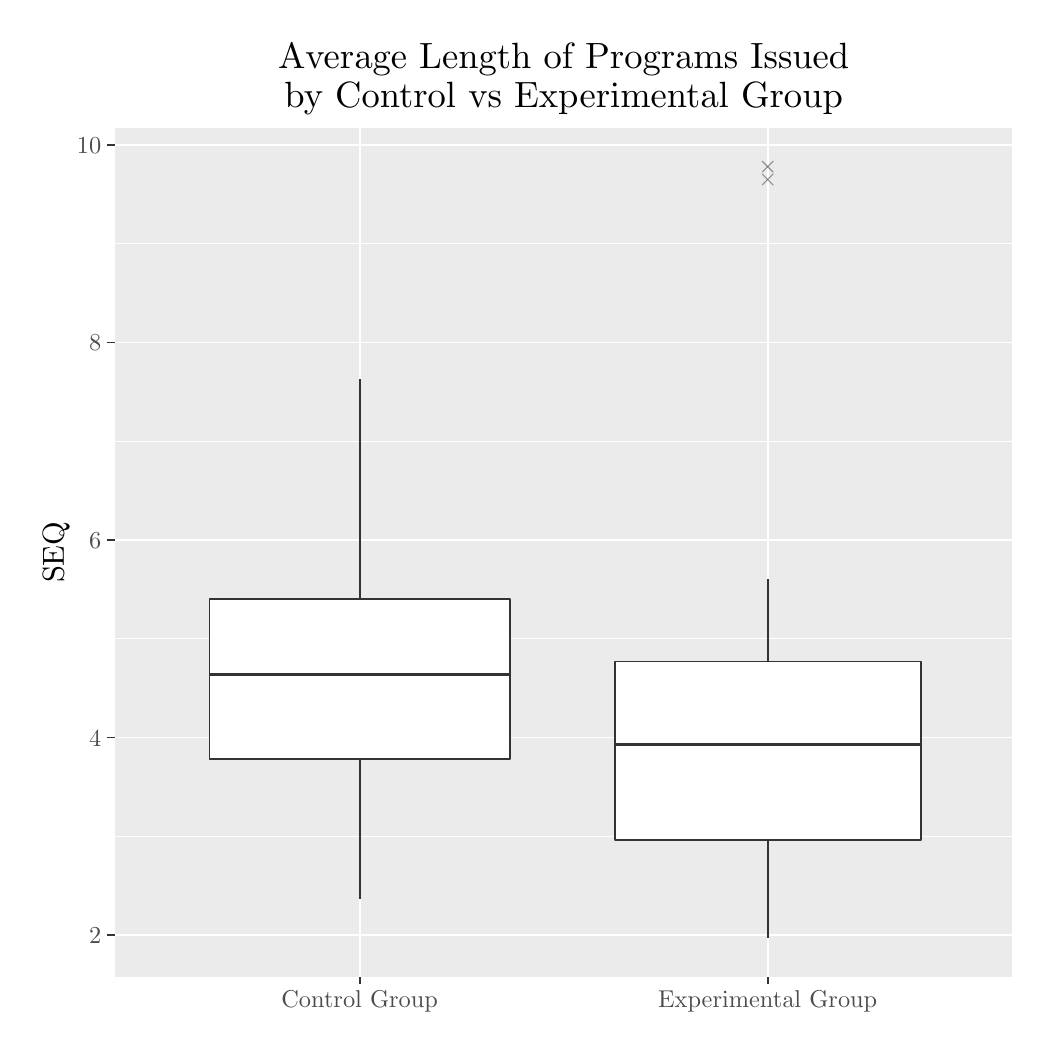
\begin{tikzpicture}[x=1pt,y=1pt]
\definecolor{fillColor}{RGB}{255,255,255}
\path[use as bounding box,fill=fillColor,fill opacity=0.00] (0,0) rectangle (361.35,361.35);
\begin{scope}
\path[clip] (  0.00,  0.00) rectangle (361.35,361.35);
\definecolor{drawColor}{RGB}{255,255,255}
\definecolor{fillColor}{RGB}{255,255,255}

\path[draw=drawColor,line width= 0.6pt,line join=round,line cap=round,fill=fillColor] (  0.00,  0.00) rectangle (361.35,361.35);
\end{scope}
\begin{scope}
\path[clip] ( 31.52, 18.45) rectangle (355.85,325.06);
\definecolor{fillColor}{gray}{0.92}

\path[fill=fillColor] ( 31.52, 18.45) rectangle (355.85,325.06);
\definecolor{drawColor}{RGB}{255,255,255}

\path[draw=drawColor,line width= 0.3pt,line join=round] ( 31.52, 69.12) --
	(355.85, 69.12);

\path[draw=drawColor,line width= 0.3pt,line join=round] ( 31.52,140.51) --
	(355.85,140.51);

\path[draw=drawColor,line width= 0.3pt,line join=round] ( 31.52,211.89) --
	(355.85,211.89);

\path[draw=drawColor,line width= 0.3pt,line join=round] ( 31.52,283.27) --
	(355.85,283.27);

\path[draw=drawColor,line width= 0.6pt,line join=round] ( 31.52, 33.43) --
	(355.85, 33.43);

\path[draw=drawColor,line width= 0.6pt,line join=round] ( 31.52,104.81) --
	(355.85,104.81);

\path[draw=drawColor,line width= 0.6pt,line join=round] ( 31.52,176.20) --
	(355.85,176.20);

\path[draw=drawColor,line width= 0.6pt,line join=round] ( 31.52,247.58) --
	(355.85,247.58);

\path[draw=drawColor,line width= 0.6pt,line join=round] ( 31.52,318.97) --
	(355.85,318.97);

\path[draw=drawColor,line width= 0.6pt,line join=round] (119.97, 18.45) --
	(119.97,325.06);

\path[draw=drawColor,line width= 0.6pt,line join=round] (267.40, 18.45) --
	(267.40,325.06);
\definecolor{drawColor}{RGB}{51,51,51}

\path[draw=drawColor,draw opacity=0.50,line width= 0.4pt,line join=round,line cap=round] (265.43,304.53) -- (269.36,308.46);

\path[draw=drawColor,draw opacity=0.50,line width= 0.4pt,line join=round,line cap=round] (265.43,308.46) -- (269.36,304.53);

\path[draw=drawColor,draw opacity=0.50,line width= 0.4pt,line join=round,line cap=round] (265.43,309.16) -- (269.36,313.08);

\path[draw=drawColor,draw opacity=0.50,line width= 0.4pt,line join=round,line cap=round] (265.43,313.08) -- (269.36,309.16);
\definecolor{drawColor}{gray}{0.20}

\path[draw=drawColor,line width= 0.6pt,line join=round] (267.40,132.27) -- (267.40,162.16);

\path[draw=drawColor,line width= 0.6pt,line join=round] (267.40, 67.74) -- (267.40, 32.39);
\definecolor{fillColor}{RGB}{255,255,255}

\path[draw=drawColor,line width= 0.6pt,line join=round,line cap=round,fill=fillColor] (212.11,132.27) --
	(212.11, 67.74) --
	(322.68, 67.74) --
	(322.68,132.27) --
	(212.11,132.27) --
	cycle;

\path[draw=drawColor,line width= 1.1pt,line join=round] (212.11,102.30) -- (322.68,102.30);

\path[draw=drawColor,line width= 0.6pt,line join=round] (119.97,154.78) -- (119.97,234.31);

\path[draw=drawColor,line width= 0.6pt,line join=round] (119.97, 96.97) -- (119.97, 46.41);

\path[draw=drawColor,line width= 0.6pt,line join=round,line cap=round,fill=fillColor] ( 65.76,154.78) --
	( 65.76, 96.97) --
	(174.18, 96.97) --
	(174.18,154.78) --
	( 65.76,154.78) --
	cycle;

\path[draw=drawColor,line width= 1.1pt,line join=round] ( 65.76,127.53) -- (174.18,127.53);
\end{scope}
\begin{scope}
\path[clip] (  0.00,  0.00) rectangle (361.35,361.35);
\definecolor{drawColor}{gray}{0.30}

\node[text=drawColor,anchor=base east,inner sep=0pt, outer sep=0pt, scale=  0.88] at ( 26.57, 30.40) {2};

\node[text=drawColor,anchor=base east,inner sep=0pt, outer sep=0pt, scale=  0.88] at ( 26.57,101.78) {4};

\node[text=drawColor,anchor=base east,inner sep=0pt, outer sep=0pt, scale=  0.88] at ( 26.57,173.17) {6};

\node[text=drawColor,anchor=base east,inner sep=0pt, outer sep=0pt, scale=  0.88] at ( 26.57,244.55) {8};

\node[text=drawColor,anchor=base east,inner sep=0pt, outer sep=0pt, scale=  0.88] at ( 26.57,315.94) {10};
\end{scope}
\begin{scope}
\path[clip] (  0.00,  0.00) rectangle (361.35,361.35);
\definecolor{drawColor}{gray}{0.20}

\path[draw=drawColor,line width= 0.6pt,line join=round] ( 28.77, 33.43) --
	( 31.52, 33.43);

\path[draw=drawColor,line width= 0.6pt,line join=round] ( 28.77,104.81) --
	( 31.52,104.81);

\path[draw=drawColor,line width= 0.6pt,line join=round] ( 28.77,176.20) --
	( 31.52,176.20);

\path[draw=drawColor,line width= 0.6pt,line join=round] ( 28.77,247.58) --
	( 31.52,247.58);

\path[draw=drawColor,line width= 0.6pt,line join=round] ( 28.77,318.97) --
	( 31.52,318.97);
\end{scope}
\begin{scope}
\path[clip] (  0.00,  0.00) rectangle (361.35,361.35);
\definecolor{drawColor}{gray}{0.20}

\path[draw=drawColor,line width= 0.6pt,line join=round] (119.97, 15.70) --
	(119.97, 18.45);

\path[draw=drawColor,line width= 0.6pt,line join=round] (267.40, 15.70) --
	(267.40, 18.45);
\end{scope}
\begin{scope}
\path[clip] (  0.00,  0.00) rectangle (361.35,361.35);
\definecolor{drawColor}{gray}{0.30}

\node[text=drawColor,anchor=base,inner sep=0pt, outer sep=0pt, scale=  0.88] at (119.97,  7.44) {Control Group};

\node[text=drawColor,anchor=base,inner sep=0pt, outer sep=0pt, scale=  0.88] at (267.40,  7.44) {Experimental Group};
\end{scope}
\begin{scope}
\path[clip] (  0.00,  0.00) rectangle (361.35,361.35);
\definecolor{drawColor}{RGB}{0,0,0}

\node[text=drawColor,rotate= 90.00,anchor=base,inner sep=0pt, outer sep=0pt, scale=  1.10] at ( 13.08,171.76) {SEQ};
\end{scope}
\begin{scope}
\path[clip] (  0.00,  0.00) rectangle (361.35,361.35);
\definecolor{drawColor}{RGB}{0,0,0}

\node[text=drawColor,anchor=base,inner sep=0pt, outer sep=0pt, scale=  1.32] at (193.68,346.76) {Average Length of Programs Issued};

\node[text=drawColor,anchor=base,inner sep=0pt, outer sep=0pt, scale=  1.32] at (193.68,332.50) {by Control vs Experimental Group};
\end{scope}
\end{tikzpicture}

  \caption{Boxplot for the average length of valid programs issued by each group.}\label{fig:avgs}
\end{figure}

Finally, the boxplot in figure~\ref{fig:avgl} shows the average number of loops issued to the robot across the two experimental groups (CYC). The average was \(0.39\) (standard deviation \(0.48\)) for learners working individually, and \(0.46\) (standard deviation \(0.5\)) for learners working collaboratively, thus as with SEQ, the difference between the two experimental groups is narrow. In this case, though, it seems that working collaboratively fosters the use of loops more than working individually, favouring \ac{CT} skills.

\begin{figure}[ht!]
  \centering
  % Created by tikzDevice version 0.12 on 2018-09-20 18:19:33
% !TEX encoding = UTF-8 Unicode
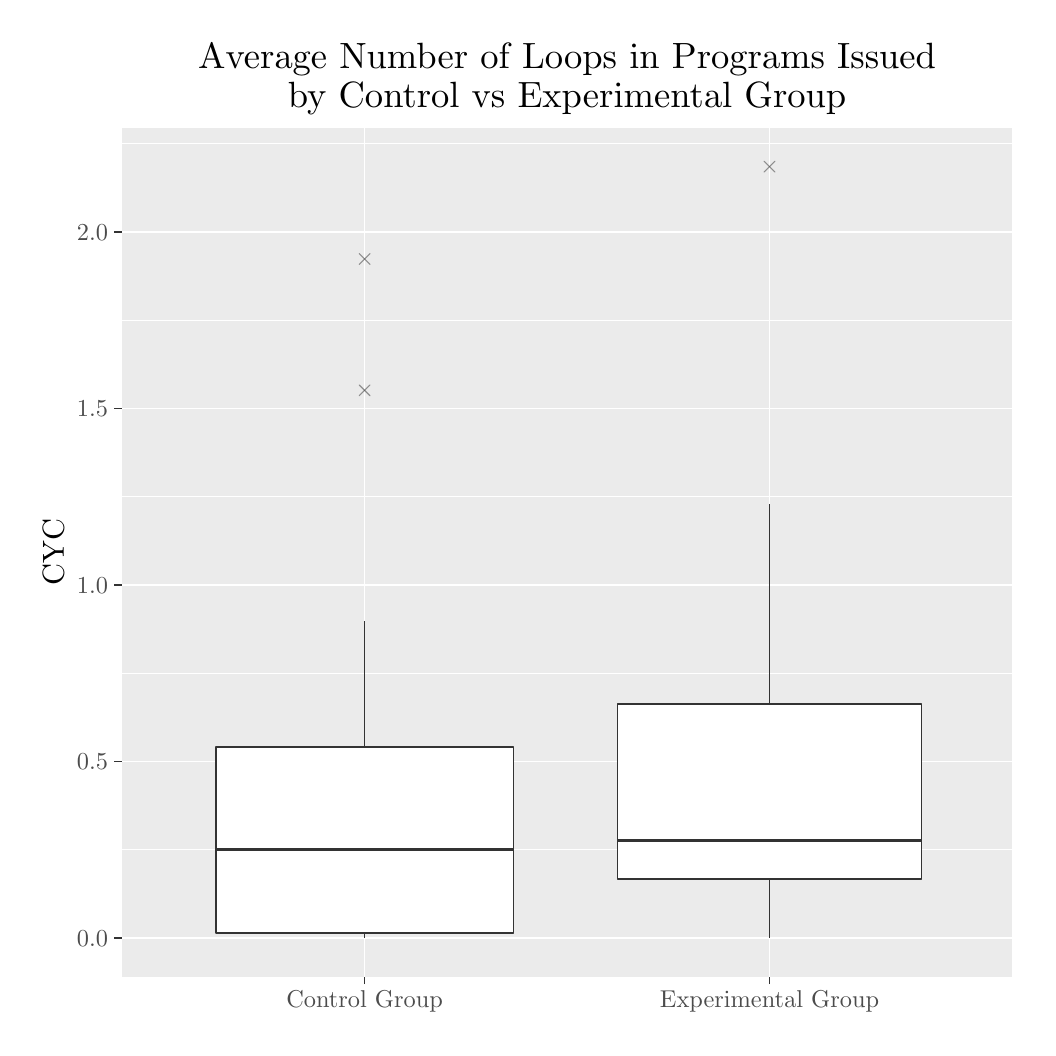
\begin{tikzpicture}[x=1pt,y=1pt]
\definecolor{fillColor}{RGB}{255,255,255}
\path[use as bounding box,fill=fillColor,fill opacity=0.00] (0,0) rectangle (361.35,361.35);
\begin{scope}
\path[clip] (  0.00,  0.00) rectangle (361.35,361.35);
\definecolor{drawColor}{RGB}{255,255,255}
\definecolor{fillColor}{RGB}{255,255,255}

\path[draw=drawColor,line width= 0.6pt,line join=round,line cap=round,fill=fillColor] (  0.00,  0.00) rectangle (361.35,361.35);
\end{scope}
\begin{scope}
\path[clip] ( 33.96, 18.45) rectangle (355.85,325.06);
\definecolor{fillColor}{gray}{0.92}

\path[fill=fillColor] ( 33.96, 18.45) rectangle (355.85,325.06);
\definecolor{drawColor}{RGB}{255,255,255}

\path[draw=drawColor,line width= 0.3pt,line join=round] ( 33.96, 64.28) --
	(355.85, 64.28);

\path[draw=drawColor,line width= 0.3pt,line join=round] ( 33.96,128.05) --
	(355.85,128.05);

\path[draw=drawColor,line width= 0.3pt,line join=round] ( 33.96,191.82) --
	(355.85,191.82);

\path[draw=drawColor,line width= 0.3pt,line join=round] ( 33.96,255.59) --
	(355.85,255.59);

\path[draw=drawColor,line width= 0.3pt,line join=round] ( 33.96,319.36) --
	(355.85,319.36);

\path[draw=drawColor,line width= 0.6pt,line join=round] ( 33.96, 32.39) --
	(355.85, 32.39);

\path[draw=drawColor,line width= 0.6pt,line join=round] ( 33.96, 96.16) --
	(355.85, 96.16);

\path[draw=drawColor,line width= 0.6pt,line join=round] ( 33.96,159.93) --
	(355.85,159.93);

\path[draw=drawColor,line width= 0.6pt,line join=round] ( 33.96,223.71) --
	(355.85,223.71);

\path[draw=drawColor,line width= 0.6pt,line join=round] ( 33.96,287.48) --
	(355.85,287.48);

\path[draw=drawColor,line width= 0.6pt,line join=round] (121.75, 18.45) --
	(121.75,325.06);

\path[draw=drawColor,line width= 0.6pt,line join=round] (268.06, 18.45) --
	(268.06,325.06);
\definecolor{drawColor}{RGB}{51,51,51}

\path[draw=drawColor,draw opacity=0.50,line width= 0.4pt,line join=round,line cap=round] (266.10,309.16) -- (270.02,313.08);

\path[draw=drawColor,draw opacity=0.50,line width= 0.4pt,line join=round,line cap=round] (266.10,313.08) -- (270.02,309.16);
\definecolor{drawColor}{gray}{0.20}

\path[draw=drawColor,line width= 0.6pt,line join=round] (268.06,117.05) -- (268.06,189.30);

\path[draw=drawColor,line width= 0.6pt,line join=round] (268.06, 53.68) -- (268.06, 32.39);
\definecolor{fillColor}{RGB}{255,255,255}

\path[draw=drawColor,line width= 0.6pt,line join=round,line cap=round,fill=fillColor] (213.19,117.05) --
	(213.19, 53.68) --
	(322.93, 53.68) --
	(322.93,117.05) --
	(213.19,117.05) --
	cycle;

\path[draw=drawColor,line width= 1.1pt,line join=round] (213.19, 67.75) -- (322.93, 67.75);
\definecolor{drawColor}{RGB}{51,51,51}

\path[draw=drawColor,draw opacity=0.50,line width= 0.4pt,line join=round,line cap=round] (119.79,275.79) -- (123.71,279.71);

\path[draw=drawColor,draw opacity=0.50,line width= 0.4pt,line join=round,line cap=round] (119.79,279.71) -- (123.71,275.79);

\path[draw=drawColor,draw opacity=0.50,line width= 0.4pt,line join=round,line cap=round] (119.79,228.34) -- (123.71,232.26);

\path[draw=drawColor,draw opacity=0.50,line width= 0.4pt,line join=round,line cap=round] (119.79,232.26) -- (123.71,228.34);
\definecolor{drawColor}{gray}{0.20}

\path[draw=drawColor,line width= 0.6pt,line join=round] (121.75,101.33) -- (121.75,146.96);

\path[draw=drawColor,line width= 0.6pt,line join=round] (121.75, 34.14) -- (121.75, 32.39);

\path[draw=drawColor,line width= 0.6pt,line join=round,line cap=round,fill=fillColor] ( 67.95,101.33) --
	( 67.95, 34.14) --
	(175.55, 34.14) --
	(175.55,101.33) --
	( 67.95,101.33) --
	cycle;

\path[draw=drawColor,line width= 1.1pt,line join=round] ( 67.95, 64.28) -- (175.55, 64.28);
\end{scope}
\begin{scope}
\path[clip] (  0.00,  0.00) rectangle (361.35,361.35);
\definecolor{drawColor}{gray}{0.30}

\node[text=drawColor,anchor=base east,inner sep=0pt, outer sep=0pt, scale=  0.88] at ( 29.01, 29.36) {0.0};

\node[text=drawColor,anchor=base east,inner sep=0pt, outer sep=0pt, scale=  0.88] at ( 29.01, 93.13) {0.5};

\node[text=drawColor,anchor=base east,inner sep=0pt, outer sep=0pt, scale=  0.88] at ( 29.01,156.90) {1.0};

\node[text=drawColor,anchor=base east,inner sep=0pt, outer sep=0pt, scale=  0.88] at ( 29.01,220.68) {1.5};

\node[text=drawColor,anchor=base east,inner sep=0pt, outer sep=0pt, scale=  0.88] at ( 29.01,284.45) {2.0};
\end{scope}
\begin{scope}
\path[clip] (  0.00,  0.00) rectangle (361.35,361.35);
\definecolor{drawColor}{gray}{0.20}

\path[draw=drawColor,line width= 0.6pt,line join=round] ( 31.21, 32.39) --
	( 33.96, 32.39);

\path[draw=drawColor,line width= 0.6pt,line join=round] ( 31.21, 96.16) --
	( 33.96, 96.16);

\path[draw=drawColor,line width= 0.6pt,line join=round] ( 31.21,159.93) --
	( 33.96,159.93);

\path[draw=drawColor,line width= 0.6pt,line join=round] ( 31.21,223.71) --
	( 33.96,223.71);

\path[draw=drawColor,line width= 0.6pt,line join=round] ( 31.21,287.48) --
	( 33.96,287.48);
\end{scope}
\begin{scope}
\path[clip] (  0.00,  0.00) rectangle (361.35,361.35);
\definecolor{drawColor}{gray}{0.20}

\path[draw=drawColor,line width= 0.6pt,line join=round] (121.75, 15.70) --
	(121.75, 18.45);

\path[draw=drawColor,line width= 0.6pt,line join=round] (268.06, 15.70) --
	(268.06, 18.45);
\end{scope}
\begin{scope}
\path[clip] (  0.00,  0.00) rectangle (361.35,361.35);
\definecolor{drawColor}{gray}{0.30}

\node[text=drawColor,anchor=base,inner sep=0pt, outer sep=0pt, scale=  0.88] at (121.75,  7.44) {Control Group};

\node[text=drawColor,anchor=base,inner sep=0pt, outer sep=0pt, scale=  0.88] at (268.06,  7.44) {Experimental Group};
\end{scope}
\begin{scope}
\path[clip] (  0.00,  0.00) rectangle (361.35,361.35);
\definecolor{drawColor}{RGB}{0,0,0}

\node[text=drawColor,rotate= 90.00,anchor=base,inner sep=0pt, outer sep=0pt, scale=  1.10] at ( 13.08,171.76) {CYC};
\end{scope}
\begin{scope}
\path[clip] (  0.00,  0.00) rectangle (361.35,361.35);
\definecolor{drawColor}{RGB}{0,0,0}

\node[text=drawColor,anchor=base,inner sep=0pt, outer sep=0pt, scale=  1.32] at (194.91,346.76) {Average Number of Loops in Programs Issued};

\node[text=drawColor,anchor=base,inner sep=0pt, outer sep=0pt, scale=  1.32] at (194.91,332.50) {by Control vs Experimental Group};
\end{scope}
\end{tikzpicture}

  \caption{Boxplot for the average number of loops issued by each group.}\label{fig:avgl}
\end{figure}

Both SEQ and CYC were not normally distributed according to the standard Shapiro-Wilk test (\(p_{SEQ} = 0.001\) and \(p_{CYC} < 0.001\)). To verify the experimental hypothesis, the one-tailed Mann-Whitney U-test was selected, which is a robust, nonparametric test.

The experimental hypothesis (\(H_1\)) predicts a difference in \ac{CT} skills development between learners working collaboratively and learners working individually. The tests were not statistically significant though (\(p_{SEQ} = 0.0658\) and \(p_{CYC} = 0.4776\)), hence the null hypothesis cannot be rejected.

\section{Discussion and Post-Hoc Analysis}
Even if the results of the experiment did not confirm the experimental hypothesis, there are interesting pointers coming from the collected data that can be helpful to explore more in-depth the main research question of this thesis and offer valid suggestions for the follow-up studies.

Results of the two evaluated measures --- SEQ and CYC --- point towards opposite effects: even though the difference is narrow, it seems that individual working groups tend to produce longer sequential programs while collaborating groups use more loops. This yet not significant effect would have been expected: by leveraging on collaboration, \acp{VPL}-based tools should foster higher-level \ac{CT} skills such as loops and abstraction, since social interactions are an important factor of constructivist learning theories, as discussed in Chapter~\ref{chap:background}. Unfortunately, the study failed to measure this sought effect (if present), and the reasons might be various and worth analysing in more detail.

First, \acp{VPL} are designed to run on traditional digital systems, which are based on a \ac{GUI} interaction paradigm: they are based on artificial control devices such as mouse and keyboard, and they don't support and take advantage of collaborative situations when multiple users are collaborating with the support of the device. A recent evolution in interaction design is indeed founded on such premise: the more modern \acp{NUI} are based on more innate human interaction paradigms such as touch, vision and speech, and are known as \emph{natural} because they rely on a user being able to carry out relatively natural motions to control the application or manipulate the on-screen content, fostering and cultivating user collaboration. Designing new and engaging tools founded on the basis of \acp{NUI} could represent a shift towards new \ac{CT} support tools, which might take more advantage of collaborative and experiential learning to better cultivate such skills.

Moreover, \ac{VPL}-based environments such as Scratch and Blockly have developed highly active online communities over the past few years, providing users with existing solutions to problems, forums to get help and discuss amongst peers, and many other resources. They were designed to take advantage of online collaboration rather than offline, representing a \ac{CT} support tool more for individual working learners, rather than collaborating ones.

The tasks provided to participants were perhaps too simple to observe a significant effect between the two experimental groups. The selected tasks were indeed real-world introductory tasks, designed to get students interested in robot programming without challenging right away inexperienced ones. Perhaps the sought effect would have been more significant with different and specifically-designed activities, but it would not have been as much grounded in existing real-world practices.

Finally, the study did not take into account more common measures such as time to task, tasks completion rates, and many other subjective measures related to attitude, engagement, and reflection. Even though these are more common measures used in the literature, the study design strived to detect \ac{CT} developments rather than programming ability. Perhaps further research on non-invasive measures of \ac{CT} skills could help highlighting this effect without designing ad-hoc evaluation tasks that might not highlight real-world effects taking place.

\section{Threats to Validity}
There are several validity threats to the design of this study.

\paragraph{Internal Validity} The limited task complexity and available time prevented a full evaluation of different \ac{CT} factors that could have influenced by the different treatments. However, the study has been conducted in a real-world scenario, with the original tasks designed by the instructors to introduce \ac{CT} to students and in their usual time schedule; even though it presents a limitation regarding research power, it offered a valid assessment of current practices and real-world effects of the evaluated tools.

\paragraph{Construct Validity} The \ac{CT} assessment was reduced to just two factors, understanding of sequences and loops; these are just two concepts related to more higher level skills defined in \ac{CT}, even though they are not explicitly mentioned by all the proposed definition outline in research. Nevertheless, these concepts were taken into account to avoid instrumenting the experiment and keep it as close as possible to real-world practices; indeed, sequences and loops comprehension can correlate with abstraction and decomposition abilities, which are two of the most mentioned \ac{CT} skills found in the literature.

\paragraph{External Validity} The results of the study can be generalized only in the context of the selected scenario, although it was carried out in a real educational setting, during an actual introductory programming session without instrumenting them. In order to generalize the findings to other scenarios though, replication studies employing different \ac{VPL}-based tools are needed.

\section{Contributions}
\replaced[comment={MP6}]{The Literature Review described in section \ref{sec:rw3} has}{Parts of the work and results described in this chapter have} been previously published in~\cite{turchi2016fostering,turchi2016human}.

\section{Conclusion}
This chapter presented an investigation on existing \ac{VPL}-based tools used in education and their effects on promoting \ac{CT} skills in a collaborative learning scenario.

A common \ac{VPL}-based system --- namely OzoBlockly --- was tested in a series of real-world introductory programming sessions, where Key Stage 3 learners collaborate to program a small robot and solve some simple tasks. The evaluation compared the effects of using such a system while collaborating with other peers and working individually, in terms of the development of \ac{CT} skills. \replaced[comment={D14}]{The study results failed to demonstrate a clear benefit of learning in collaborating groups over individual working ones in terms of \ac{CT} skills development. This requires further investigation, however it could point out how existing \ac{CT} tools favour offline collaboration, but are not specifically designed to support online collaborative learning}{Contrarily to what was expected, the results of the study did not highlight a significant benefit for collaborating groups, perhaps highlighting a lack of support to online collaboration by such tools, in favour of an offline one}. Designing tools to support online collaboration to foster \ac{CT} skills is indeed important and worth investigating whether different an interaction paradigm --- such as \acp{TUI} --- could be used to make this happen.

In the next chapter, the main research question of this thesis about the effects of tangible interaction on the development of \ac{CT} skills will be investigated in a specific application domain, namely \ac{IL} environments, where learning is self-directed and takes place as people go about their daily activities.                 % INCLUDE: education
% !TeX root = ../thesis.tex
%
\setcounter{chapter}{3}
\chapter{Fostering Com\-pu\-ta\-tion\-al Think\-ing Skills in In\-for\-mal Learn\-ing Do\-mains}\label{chap:tapas}

\cleanchapterquote{Children learn best when they are actively engaged in constructing something that has a personal meaning to them --- be it a poem, a robot, a sandcastle, or a computer program.}{Seymour Papert}{}

The previous chapter focused on the existing tools used in education and their effects on promoting \ac{CT} skills. This chapter carries on with the main thesis investigation over the effects of tangible interaction on the development of \ac{CT} skills and focuses on a specific application domain, namely \ac{IL} environments, where learning is mostly self-directed and takes place as people go about their daily activities, driven by their preferences and intentions.

\section{Introduction}
\deleted[comment={MP5, D16}]{As discussed in chapter 1, due to the increasingly ubiquitous presence of software in our lives, \ac{CL} and coding have become much-needed skills to possess for an ever wider audience. Nonetheless, the familiarity with highly abstract concepts required by programming still constitutes a significant entry barrier to a widespread appropriation of technology for the general public. Yet, the important role played by such skills in mundane life is not solely related to programming itself, but to their link to \ac{CT} skills, namely all those thinking abilities reflecting core concepts of \ac{CS}. This set of skills can provide people with a mental Swiss army knife that enables them to actively participate and address today's challenges with the help of modern technological tools.}

\deleted{In seeking new ways of promoting \ac{CT} skills to an ever-growing public, one might play on activities people are naturally good at, leveraging on their familiarity to lower the existing entry barrier: according to the constructivist theories of Jean Piaget~\cite{Piaget:1969vq}, exploiting human's innate dexterity for objects manipulation in the physical world and its afforded social interactions could be an effective way of aiding users in practising the abstract concepts underpinning \ac{CT}. Physical manipulation sits at the core of \acp{TUI}, a digital interaction paradigm designed with the aim of providing users with an easy to use interface that can benefit inexperienced people. Such a paradigm, often used to support the interaction of young children with technology in the classroom, could be employed to promote \ac{CT} skills by providing users with a physical representation of the concepts involved~\cite{McNerney:2004jc,Horn:2009be}, acting as a scaffold between the real world and digital~\cite{Wang:2014jy}.}

\deleted{To recap, from this context discerns the main Research Question addressed by this thesis: \textit{``Can the collaborative and cognitive naturalness of physical objects manipulation at the basis of \acp{TUI} aid the understanding of core algorithmic principles and thus improving \ac{CT} skills?''}.}

\replaced{As mentioned in chapter \ref{chap:intro}, s}{S}upporting users in cultivating their \ac{CT} skills and --- more generally --- going through their routine learning experiences is particularly relevant in \ac{IL} scenarios, namely environments where learning is predominantly unstructured, experiential, and noninstitutional, i.e.\ outside of the classroom (e.g., in museums or workplaces). Modern education strives to make learning intrinsically driven, that is by making learners responsible for their own academic explorations, thus fostering appropriation of their own learning; this way their experience becomes more self-directed and personalised, increasing both their motivation and its efficacy. Developing both technological tools and methods to promote \ac{CT} skills in \ac{IL} domains puts learners in charge and integrates learning in their daily routines to exploit their motivations and provide a more effective experience. Physical objects manipulation might help to lower the barriers of \ac{CT} and support users in dealing with such abstract concepts during \ac{IL} activities.

The Research Question derived from this context and addressed by this chapter is then: \textit{``Can physical objects manipulation help foster \ac{CT} skills in \ac{IL} domains?''}.

To properly study and address this question, this chapter introduces \acr{TAPAS}, a system combining its digital and physical features to promote \ac{CT} skills, built on the findings of the previous chapter, the literature, and a user study, that can be repurposed to different \ac{IL} scenarios.

The contributions reported in this chapter are threefold.
\begin{itemize}
  \item First, an early design of \ac{TAPAS} is described, stemming from the results of a workshop carried out with expert designers to collect insightful ideas and design challenges related to the development of a \ac{TUI}-based system that can be repurposed to different \ac{IL} domains.
  \item Second, the results of a study conducted with the preliminary prototype of \ac{TAPAS}~\cite{Turchi:2015dr,Turchi:2015kr} are reported, whose findings were used to inform its design to target \ac{IL} domains.
  \item Third, some of the main challenges faced by supporting \ac{CT} skills with objects manipulation in \ac{IL} domains are reported, based on insights from the studies that have been carried out.
\end{itemize}

\section{Related Works}\label{sec:tp}
Much of the existing body of research within the \ac{EUD} area about \acp{TUI} has focused on education. Many theories, including the constructivist ones, report the benefits of making interfaces tangible and moving them into the physical world; several studies report on their benefits for children in the classroom since they are built on experience from the real world. Providing real evidence supporting their value for educational use is quite a challenging task, although some recent studies are trying to characterise them more in detail, as this thesis seeks to do with their effects on \ac{CT} skills.

The existing literature on employing \acp{TUI} within an educational domain to foster programming-related skills can be clustered in two main categories according to the paradigm employed: \ac{PbD} or \ac{PbI}. \ac{PbD}, also known as Programming by Example, enables users to teach new behaviours to the system by demonstrating actions on concrete examples~\cite{2001:YWM:369505}. \ac{PbI}, known as Tangible (sometimes Physical) Programming within the \ac{TUI} domain, takes a traditional approach to programming, that is requiring users to learn and employ a syntactic construct (e.g., text instructions, visual or natural language) to impart instructions to the system. This makes the \ac{PbI} paradigm less coupled with the operational domain it is applied to, whilst \ac{PbD} is directly linked to it by having users manipulate only their artefacts.

Topobo~\cite{Parkes:2008bu} --- proposed by Parkes et al. --- falls under the first category and comprises a set of components that one can assemble and animate with different manipulations; the system then repeatedly plays those motions back. \ac{PbD} proved to be an effective and intuitive way of teaching different movements to a system directly on actuated physical objects, therefore it has been specifically named Robot Programming by Demonstration~\cite{Billard:2008kb}. The system devised by Lee et al.~\cite{Lee:2013gya} uses a different approach: this \ac{PbD} system allows users to record macros composed by physical and digital actions performed on several objects, such as opening a drawer, turning on the TV, and so on; the system records the actions' sequence and plays them back in the same order once the first action is performed.

These systems offer an unparalleled experience in terms of ease of use, but --- due to the paradigm they employ --- present a quite substantial limitation: users can interact only with the outputs, therefore the instructed behaviours are necessarily composed solely of operations that are directly available, resulting in the inability to represent more complex behaviours; this is the reason why the main problem of \ac{PbD} systems is the generalizability --- i.e.\ finding the general semantics --- of instructed behaviours~\cite{2001:YWM:369505}.

Moving to \ac{PbI}-based systems, Mugellini et al.~\cite{Mugellini:2009gl} proposed the concept of tangible shortcuts: they improved information access and retrieval using physical objects, enabling users to develop new shortcuts through a Visual Language based on a puzzle metaphor. Wang et al.~introduced E-Block~\cite{Wang:2012cp}, a tangible programming tool for young children, enabling them to instruct a robot's movements by assembling different blocks, each assigned to a specific function. Robo-Blocks is a similar system presented by Sipitakiat and Nusen~\cite{Sipitakiat:2012cba}, which added the ability for users to debug their applications using a display placed on top of each block.

The effects of employing a \ac{TUI} to interact with a digital system are certainly dependent on the tasks and domain, as many comparative studies suggest~\cite{Weiss:2009ct, Muller:2014kx, Hancock:2009bg}; for this reason, Kirk et al.~\cite{Kirk:2009ue} made the case for hybrid surfaces, employing physical elements together with digital ones. 

\section{Tangible Programming in Informal Learning Domains}
As discussed in the introduction, \ac{IL} is a very effective form of learning that fosters appropriation by allowing users to self-pace their experience outside of the traditional classroom. Technological tools and methods can assist learners through their self-directed journey, particularly when the goal is to promote \ac{CT} skills. Also, by allowing such tools to exploit humans' natural dexterity for objects manipulation as implied by constructivist theories, they might further support learning of the abstract concepts underpinning \ac{CT} within such domains.

The design of technological tools enhancing \ac{CT} skills within \ac{IL} domains is influenced by some \emph{key factors} concerning these scenarios. As reported in~\cite{doi:10.1177/152342239900100302}, \ac{IL} is
\begin{enumerate*}[label=(F\arabic*)]
  \item integrated with learners' daily routines,
  \item triggered by an internal or external jolt,
  \item not highly conscious,
  \item influenced by chance,
  \item an inductive process of reflection and action, and
  \item linked to the learning of others.
\end{enumerate*}
Leveraging on these factors when designing a new tool allows for an optimal support of learning activities in such environments and limits its casual nature.

In this chapter, a new tool supporting \ac{IL} of \ac{CT} skills is proposed, which
\begin{itemize}
  \item is a software platform --- namely a system designed to run different applications --- thus it can be repurposed to different scenarios, integrating into learners' heterogeneous daily routines (F1);
  \item supports inductive processes (F5) by providing users with an \ac{EUD} environment where they can iteratively assemble different workflows --- namely sequential processes combining different small applications in a step-by-step data-flow fashion, where the output of an application becomes the input of the following one.
  \item supports collaboration (F6) by implementing a \ac{TUI} on a tabletop display --- namely an interactive display system, naturally fostering users collaboration by providing multiple physical interaction points placed on a horizontal surface for them to play with.
\end{itemize}

In the next section, the process of designing such a platform is outlined, starting with a focus group with designers to devise a first preliminary design.

\subsection{Preliminary Study}\label{sec:pstudy}
Several design choices have to be made to design a platform with tangible controls that need to be easily integrated into many different \ac{IL} scenarios. For this reason, an early focus group with experts was run to collect ideas and suggestions to drive the design choices.

Five experts with backgrounds in different design areas were gathered in a university meeting room for a one-hour session: three experienced interaction designers with some basic programming knowledge --- one with a specific background on information visualization and one with quite substantial industry experience --- and two product designers without any programming experience at all.

\begin{figure}[ht!]
\centering
\includegraphics[width=0.7\textwidth]{images/c4/IFTTT.png}
\caption{An example of a workflow created using \ac{IFTTT}: when the condition in the user's location changes to rain (trigger) it will automatically post a tweet (action).}\label{fig:ifttt}
\end{figure}

During the first phase --- lasting 30 minutes --- participants were instructed in the context of this research and the problem it is addressing by the facilitator. They were shown some videos outlining the process of developing workflows on \acr{IFTTT}~\cite{IFTTT}, a widely popular \ac{EUD} Web mashup system~\cite{Malizia:2011tw}; it allows users to create simple event-based \emph{if-then}-style workflows with different Web services and acts as a hub connecting their events' triggers with actions: one can describe simple rules by selecting the event that will trigger the workflow (e.g., when the current temperature rises above a certain value or when the user edits a specific file on Dropbox) and an action that should be performed by any other --- even the same --- supported Web service (e.g., tweet about it or send the file via email), as shown in figure~\ref{fig:ifttt}. This platform is very flexible and can be easily integrated into most people day-to-day activities on the Web to support them. Thus, it was chosen to showcase different types of simple workflows, their inner logic and how the trigger selection provides the subsequent action with anchors dependent on the output's type: for instance, when the event concerns a location the action can access its GPS coordinates, when it involves a text file the action will be able to use its content, and so on.

Then participants were shown a video of an existing \ac{TUI} system --- the Tangible 3D Tabletop~\cite{Dalsgaard:2014ut} --- which summarized the benefits of this interaction paradigm. In particular, two different ways of employing tangible objects in educational systems were shown~\cite{Zuckerman:2005:ETI:1054972.1055093}, in order to prompt them to produce different ideas: \acp{FiM} are building blocks used to design and represent real-world things, objects, and physical structures, for example, 3D building blocks to represent buildings on a map (figure~\ref{fig:tangible:a}). \acp{MiM} are building blocks focused on modelling more conceptual and abstract structures, for instance, tangibles used to control RGB colour blending (figure~\ref{fig:tangible:b}).

\begin{figure}[ht!] 
  \begin{subfigure}[b]{0.48\linewidth}
    \centering
    \includegraphics[width=0.75\linewidth]{images/c4/BuildingTangible.jpg} 
    \caption{3D building fa\c{c}ades on tangibles placed on a map.}\label{fig:tangible:a}
    \vspace{6ex}
  \end{subfigure}
  \begin{subfigure}[b]{0.48\linewidth}
    \centering
    \includegraphics[width=0.75\linewidth]{images/c4/RGBTangible.jpg} 
    \caption{Three tangibles used as RGB colour blenders. The base colour is projected onto each tangible, and users can change the hue of the triangle drawn within the tangibles by turning them.}\label{fig:tangible:b}
  \end{subfigure}
  \caption{Two examples of different metaphors involved in the Tangible 3D Tabletop system~\cite{Dalsgaard:2014ut}.}\label{fig:tangible}
\end{figure}

After the introduction, participants started a 30-minute discussion about ideas and challenges for the design, focusing on an \ac{IL} scenario involving users with no previous programming experience. The gathered feedback is summarised in the following.

\subsubsection{Study Findings}
The features suggested by participants were clustered by subject --- concerning either the system's tangible objects or its digital syntax. Here are the main findings from the focus group:

\paragraph{Tangible features} Participants remarked the fact that the system should react only upon user actions and provide useful feedback through a specific communication channel, in agreement with one of the main principles of \acp{NUI}~\cite{Wigdor:2011bi}. Many suggestions focused on the preferred channel to be used to provide feedback. These included providing tangible objects with a touch-sensitive mechanism in order to activate the feedback only when users physically touch objects on the table, in order to highlight whether selected objects are compatible with each other (fulfilling the workflow constraints). Moreover, the feedback communication channel of choice can be a physical one as well: a magnetic attraction between objects could indicate whether two workflow's components are compatible with each other, while repulsion might represent the opposite. An\-oth\-er par\-tic\-i\-pant sug\-gest\-ed employing haptic feedback built into the tangibles to communicate compatibility between different ones.

\paragraph{Digital features} Another set of suggestions were directed towards the digital representation of the platform's syntax. First, the blocks' digital representation should help users understand components' constraints by using, respectively, different and similar colours or shapes for incompatible and compatible components. Also, since a workflow's composition is usually performed one component at a time, i.e.\ by selecting a function that will follow the latest assembled one, the system shall aid users on the next available components to be chosen by changing the colour or the shape of the currently assembled workflow. Lastly, available components should be displayed all at once, giving users an overall view of the system's capabilities. However, this can also increase mistakes. Since the target group is inexperienced users, the system should assist them in finding the right way of assembling different components, when they cannot figure it out themselves; a useful suggestion on this regard is to provide some sort of ``translation tool'', which --- once a user selects two blocks incompatible with each other --- shows them at least one possible way of choosing other components in between to connect the two blocks, assisting users during the composition phase.

The suggestions stemming from the workshop drove a preliminary design of the system, whose details are presented in the next section.

\subsection{Preliminary Design}\label{sec:pdesign}
The system design aims to provide users with a platform that can be employed in a variety of \ac{IL} domains --- e.g., in museums or workplaces --- to cultivate \ac{CT} skills through objects manipulation.

The platform is deployed on tabletop displays, which naturally foster collaboration as required in \ac{IL} domains, and consists in a Block-based Programming environment~\cite{Mohamad:2011kz} to support inductive processes --- widely used in systems like Scratch~\cite{Resnick:2009bd} and Blockly~\cite{BLOCKLY} --- that has proven to have a low learning threshold for non-programmers, as thoroughly discussed in the previous chapter.

It allows users to create, share, modify and reuse simple workflows, namely sequential processes combining different services in a data-flow fashion, where the output of a service becomes the input of the following one, integrating into users' daily routine while supporting \ac{IL} through inductive processes. 

Users impart instructions through a visual syntactic construct in a \ac{PbI} fashion rather than by demonstrating their intentions to the system: indeed, making a workflow's inner architecture transparent to users can help them to better understand its sequential logic and behaviour, providing further design opportunities to improve their \ac{CT} skills and easily integrate the system into rather different scenarios.

The system's blocks correspond to workflow components (i.e.\ functions) that can be assembled together as in many other Block-based Programming environments; each block receives specific formats of data as input and produces different ones as output based on its inner workings and its location within a workflow's logic. Type constraints on different blocks inputs and outputs are afforded using different shapes, as in a puzzle.

A tangible object is associated with the main block --- a circle halo with a single hollow to accommodate the next piece to be added to the workflow --- which will move alongside the object on the main display's surface; moving the main piece towards another will add the latter's related function to the workflow --- only if the two shapes are matching, that is to say, the latest output is compatible with the required input (figure~\ref{fig:walkthrough:a}). This mechanism aids end-users in understanding the data-flow approach as well as type constraints.

Inputs requested by services might be quite heterogeneous and complex depending on the scenario, requiring at this point a precise and familiar input mechanism that can adapt to different needs. Hence, smartphones have been se\-lect\-ed as the tan\-gi\-bles controlling the main blocks in the system: they represent objects whose movements allow users to interact with the system, i.e.\ they form the physical and digital representation of information in the system, and are already equipped with all the sensors and feedback mechanisms needed to implement the designers' suggestions obtained from the focus group and push the interaction even further. They can be used to adapt the system to the different users' preferences since they hold much of their personal information. Moreover, they can be used to display a wide range of widgets that can be presented to end-users depending on the specific service being accessed (e.g., a virtual keyboard for text input).

\begin{figure}[ht!]
\centering
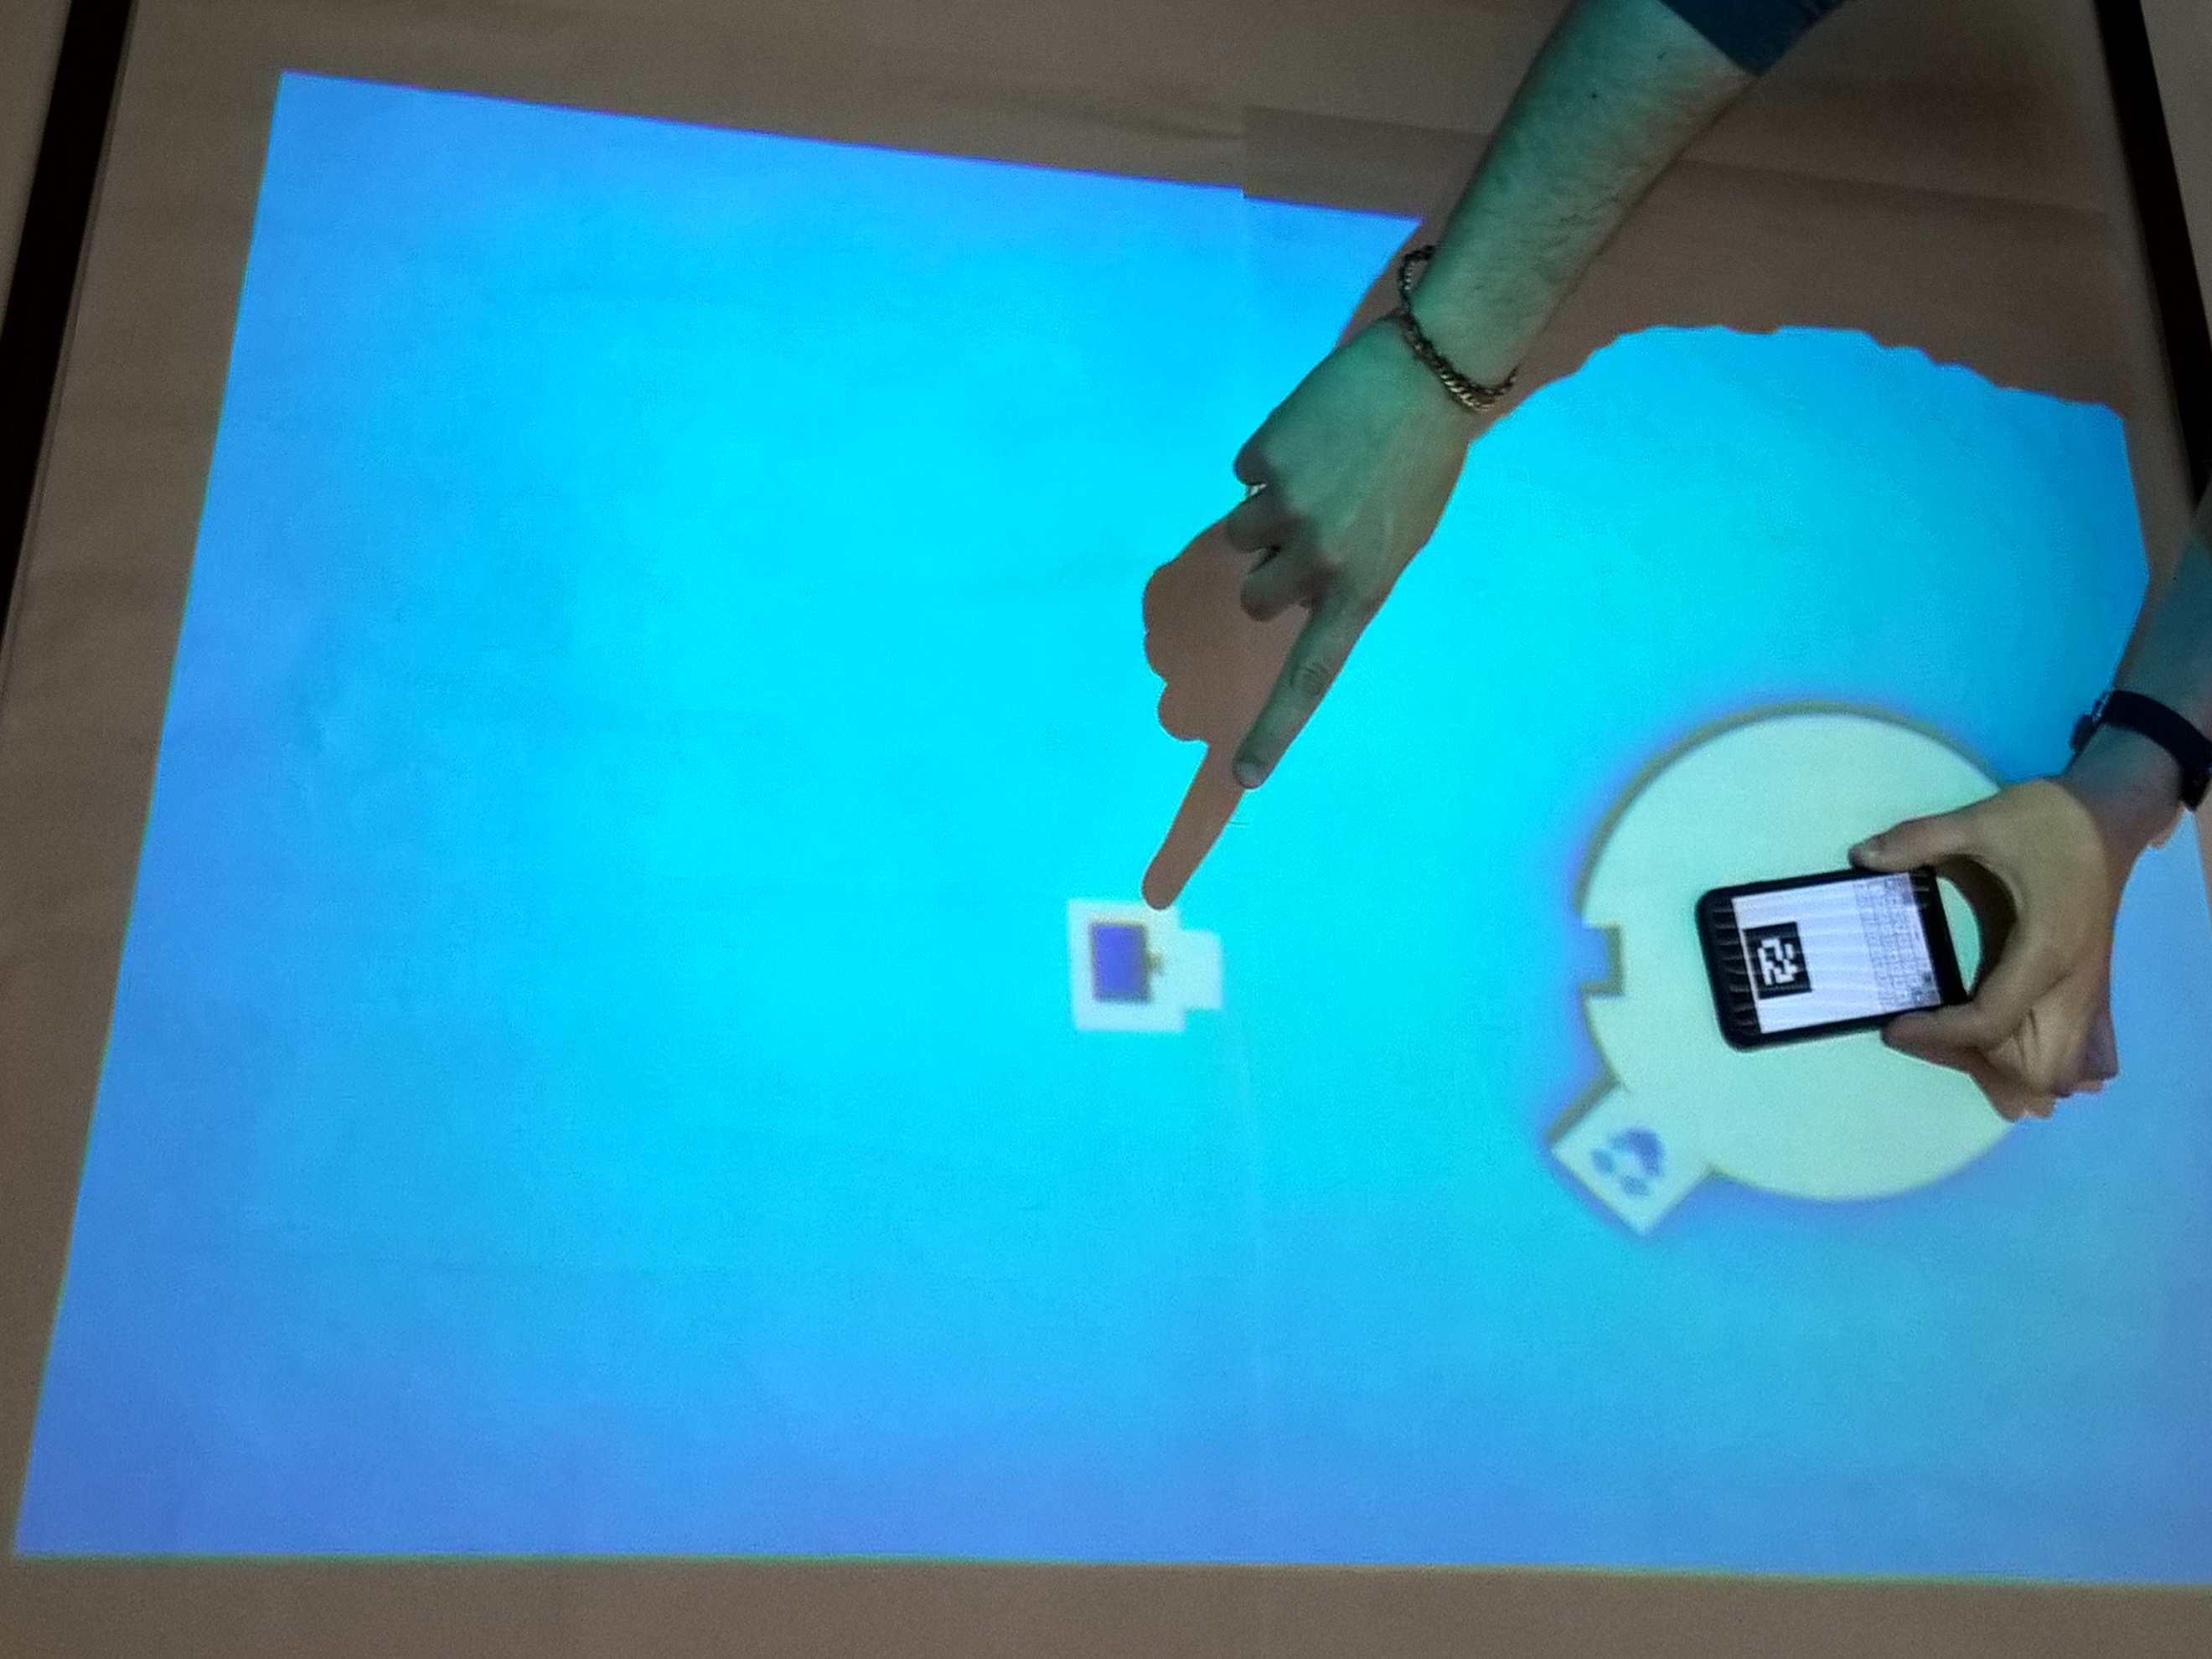
\includegraphics[width=0.7\textwidth,trim={800 100 0 100},clip]{images/c4/protopic.png}
\caption{An example of a workflow being assembled using the proposed system: a keyboard widget is displayed on the smartphone once a new piece requiring an input is assembled.}\label{fig:proto}
\end{figure}

Widgets vary depending on the type of input requested: selecting a single option among several will prompt the user with a list box, a single action to be performed will display a button, and a generally unstructured raw text to be inserted will present a keyboard (figure~\ref{fig:proto} and~\ref{fig:walkthrough:b}). Once a user enters the requested input on a widget, the latter disappears from the smartphone and the projected halo surrounding it opens up a new hollow to allow for the next block to be inserted (figure~\ref{fig:walkthrough:c}); then using the input, only the hollow that is compatible with it is displayed, preventing invalid compositions. When a workflow is completed, it can be run by pressing a button on the smartphone (figure~\ref{fig:walkthrough:d}).

\begin{figure}[ht!] 
  \begin{subfigure}[b]{0.48\linewidth}
    \centering
    \includegraphics[width=0.75\linewidth,trim={800 200 1600 200},clip]{images/c4/TAPAS-1.png} 
    \caption{The first piece is se\-lect\-ed and add\-ed to the cur\-rent work\-flow by mov\-ing the smart\-phone to\-wards it.}\label{fig:walkthrough:a}
  \end{subfigure}\hfill
  \begin{subfigure}[b]{0.48\linewidth}
    \centering
    \includegraphics[width=0.75\linewidth,trim={800 200 1600 200},clip]{images/c4/TAPAS-2.png} 
    \caption{The cor\-re\-spond\-ing widg\-et is dis\-played on the smart\-phone wait\-ing for us\-er in\-put.}\label{fig:walkthrough:b}
  \end{subfigure}
  \begin{subfigure}[b]{0.48\linewidth}
    \centering
    \includegraphics[width=0.75\linewidth,trim={800 200 1600 200},clip]{images/c4/TAPAS-3.png} 
    \caption{Once the in\-put is in\-sert\-ed, a piece whose in\-put match\-es the cur\-rent work\-flow's out\-put can be add\-ed.}\label{fig:walkthrough:c}
  \end{subfigure}\hfill
  \begin{subfigure}[b]{0.48\linewidth}
    \centering
    \includegraphics[width=0.75\linewidth,trim={800 200 1600 200},clip]{images/c4/TAPAS-4.png} 
    \caption{Fi\-nal\-ly, the work\-flow is com\-plet\-ed and the us\-er can run it from her smart\-phone.}\label{fig:walkthrough:d}
  \end{subfigure}
  \caption{A step-by-step walkthrough of building a workflow.}\label{fig:walkthrough}
\end{figure}

The next section reports a study carried out to evaluate the platform and address the Research Question formulated in the introduction of this chapter related to the effects of physical manipulation on the development of \ac{CT} skills in \ac{IL} domains.

\section{Evaluation}\label{sec:ev4}
This section presents the goals, hypotheses, and description of the experiment carried out to test the designed system, following the guidelines of the American Psychological Association~\cite{Wohlin:2000:ESE:330775}.

\subsection{Goals}
The goal of the experiment is to evaluate the system design and tangible-based interaction paradigm in a real-world \ac{IL} scenario, namely a work project meeting. The purpose is to evaluate whether this system might be employed in a given \ac{IL} scenario and investigate the effects of \ac{TUI} on the development of \ac{CT} skills.

\subsection{Research Question}
\ac{CT} is a set of skills that can help people  play a more active role in their day to day life, due to the massive impact of software in today's Information Society. Nonetheless, people struggle in dealing with the abstract concepts underlying it, thus it is important to support them in fostering such skills with new and engaging ways without getting in between their actual routine. Constructivist theories suggest that objects manipulation --- underpinning \acp{TUI} --- might be an effective way of aiding end-users in making such highly abstract concepts more tangible and understandable.

Supporting users in developing \ac{CT} skills is even more important in \ac{IL} scenarios, where learning is predominantly unstructured, experiential, and noninstitutional, making the experience self-directed and personalised with higher motivations and efficacy. 

Promoting \ac{CT} skills in \ac{IL} domains through physical objects manipulation might help to lower the barriers of \ac{CT} by integrating learning in their daily routines and supporting users in dealing with such abstract concepts through their day-to-day experiences.

The proposed system has been developed with the aim of investigating the influence of \acp{TUI} on \ac{CT} skills in multiple \ac{IL} scenarios. It employs a tangible-based interaction with a tabletop surface --- naturally fostering collaboration --- and supports inductive processes by means of assembling workflows to solve simple tasks. Thus, it has been designed to easily integrate into users' day-to-day routine to support \ac{CT} skills.

The main research question addressed by the evaluation is then \textit{``Can physical objects manipulation help foster \ac{CT} skills in \ac{IL} domains?''}.

\subsection{Experiment Design}
Due to the openness of the range of scenarios analysed --- i.e.\ \ac{IL} scenarios --- an exploratory research design was used, comprising two phases:
\begin{enumerate}
  \item a combination of oral feedback and observations of end-users engaging with the prototype in a semi in-the-wild scenario, i.e.\ taking place in a real-world setting and addressing real-world problems, as a way of testing it in a generic \ac{IL} environment, and
  \item semi-structured interviews of domain experts, in order to gather more generic and less domain-specific feedback.
\end{enumerate}

\subsection{Participants}
\subsubsection{First Phase}
The study involved end-users selected among Brunel University second-year students in the Department of Computer Science, College of Engineering and Design. As part of their degree they are clustered into groups of 4-6 and tasked with an Android application development project to be undertaken during the course of the year; they are required to meet and work collaboratively every week, normally in the library or in one of the college's meetings rooms, and can use a range of available tools to work together and share information with each other (online dedicated forums or drives, laboratory spaces with coding facilities, etc.). The development is supervised by a teaching staff member, whom they usually meet all together as a group once a week. The objective of these meetings is not to develop the Android application --- which is an individual task --- but to coordinate and organize a project plan, eventually designing a Gantt diagram to split the workload into individual tasks. This is a time when students self-direct their activities, exchange suggestions, and support each other, being a proper example of a real-world \ac{IL} scenario.

In particular, three groups of students in their second year participated to the study, made up respectively of four (1 female, 3 males), five (1 female, 4 males), and six (all males) students, reflecting the real project activity requirements and average group size; participants had no prior knowledge of the system, but attended their introductory programming course during their first year, thus they already had some programming and problem-solving experience.

\subsubsection{Second Phase}
Three interaction design experts were involved to get feedback on the featured modality; they were composed of two HCI experts --- with a mixture of academic and industry backgrounds --- and a product designer, all with more than 20 years of experience in their fields. By involving more experienced participants, the proposed interaction modality has been further evaluated through a less domain-specific point of view, considering a wide range of \ac{IL} domains for its application.

\subsection{Settings and Procedure}
\subsubsection{First Phase}
The study took place within the University facilities, in a room inside the Department of Computer Science designated to students and staff meetings, where many public interactive displays are already being deployed and used with a researcher present. It was conducted in three different sessions, one for each group of students, lasting half an hour each, and was a preliminary evaluation of the system's feature set and interaction modality.

Due to the inexperience of participants for this phase, eliciting the discussion around the system interaction modality might not have been easily gathered employing only a paper and pencil approach. Thus, students were prompted with it as a ``provotype'' --- i.e.\ a provocative prototype, namely a prototype that deliberately challenges stakeholders' conceptions by reifying and exposing tensions of existing practice in a context of interest~\cite{Boer:2012ku}; this includes a small set of features highly tailored to the evaluation scenario (i.e.\ university students collaborating with each other).

The features made available to participants, each rendered with a different block, were:
\begin{enumerate*}[label={(\arabic*)}]
  \item selecting and downloading a file from the user's Dropbox account;
  \item displaying a downloaded PDF file or an image on the main tabletop screen;
  \item searching for a book in the university library and retrieving its location inside the building depicted in an image; and
  \item sending a text document to a specified email address.
\end{enumerate*}

For instance, one could pick 1 and 2 (in this order) and the composed application would download a PDF from the user's Dropbox folder and display its content on the big screen (as depicted in figure~\ref{fig:walkthrough}); composing 3 and 2 together would result in looking for an available book in the university library and displaying its location on the big screen.

\begin{figure}[ht!]
\centering
\includegraphics[width=0.7\textwidth]{images/c4/studs.png}
\caption{One of the participating groups to the study.}\label{fig:studs}
\end{figure}

Each session lasted 30 minutes and started by briefly introducing the current version of the system to participants, explaining to them how the system works. They were then left to play with it for 15 minutes (figure~\ref{fig:studs}), and finally, a semi-structured interview was carried out, mainly focused on the proposed interaction modality.

\subsubsection{Second Phase}
Semi-structured interviews were carried out in a controlled environment (figure~\ref{fig:des}), namely during a workshop on the island of Tiree, during the bi-annual Tiree Tech Wave, a gathering of experts in various fields, ranging from interaction designers and artists to computer scientists.

\begin{figure}[ht!]
\centering
\includegraphics[width=0.7\textwidth]{images/c4/tiree.png}
\caption{The designer study setting.}\label{fig:des}
\end{figure}

Individual sessions lasted 45 minutes, starting by introducing the prototype, explaining the rationale behind its design and the targeted scenarios; it was then followed by a brief demonstration of how it works, going through some examples of its usage in real-world \ac{IL} scenarios. Finally, a semi-structured interview was carried out focusing on the strengths and weaknesses of the prototype in relation to the interaction modality and its applicability in \ac{IL} domains to foster \ac{CT} skills, more precisely covering the easiness of the puzzle metaphor, the use of smartphones as tangible objects, future application scenarios, and missing features.

\subsection{Summary}
\added[comment={MP3, MP8, D18}]{To recap, table \ref{tab:ch4summary} presents a summary of the specific \ac{CT} dimensions as defined in~\cite{Brennan:2012} examined in the evaluation, along with the related assessment approach, as reported in chapter \ref{chap:background}.}

\begin{table}[ht!]
  \caption{Summary of the specific \ac{CT} dimensions~\cite{Brennan:2012} considered by the evaluation with the related assessment approach.}\label{tab:ch4summary}
  \centering
  \begin{tabular}{M{0.2\linewidth}m{0.5\linewidth}M{0.2\linewidth}}
    \toprule
    \textit{\ac{CT} Dimension} & \textit{Description} & \textit{Assessment} \\
    \midrule
    Concept: sequences & Ex\-press\-ing a par\-tic\-u\-lar ac\-tiv\-i\-ty or task as a se\-ries of in\-di\-vid\-u\-al steps or in\-struc\-tions that can be ex\-e\-cut\-ed by the com\-put\-er. & Project Analysis (First Phase Provotype) \\
    Practice: abstracting and modularizing & Building something large by putting together collections of smaller parts. & Artefact-Based Interviews (First Phase Interviews) \\
    \bottomrule
  \end{tabular}
\end{table}

\added{Moreover, the second phase of this evaluation preliminarily investigated over the interaction modality of \ac{TAPAS}.}

\section{Results}
Data collected in both phases were analysed by performing a content analysis on the gathered feedback and observations.

\subsection{First Phase}
Overall results point out how the proposed user experience was considered quite satisfactory by participants; as expected, students' feedback mostly focused on missing features and the interaction with the system.

Each group managed to successfully assemble (at least once) two workflows while they were playing with it: the first one started with downloading a PDF file from a Dropbox account and displaying a preview on the main tabletop surface, while the second one started with looking for a specific book in the university library and depicting its location on the main screen.\deleted[comment={D19}]{ One group even assembled a more complex workflow, consisting of downloading a text file from Dropbox and sending it via email to an address of choice.}

From the gathered feedback it seems that a \ac{TUI} is an easy and effective way of interacting with the system throughout the composition of a workflow. Even though all participants are \ac{CS} undergraduates, their second-year group project is their first chance of tackling a wider problem-solving scenario, unlike their first year's individual development of smaller applications. This more complex project requires them to learn abstraction and decomposition skills, whilst collaborating with peers. Using the puzzle metaphor and workflows together with tangible interaction \replaced{helped}{seemed to help} them build the required \ac{CT} skills: for instance, collaboratively planning and designing the application's tasks and assigning them to each participant \replaced[comment={D20}]{could be}{seems like} a suitable scenario to practice abstraction and composition skills. Moreover, as with API development, the recipe metaphor provides different levels of transparency and abstractions useful to generalize the problem, whilst assembling blocks might help with decomposing a bigger problem into smaller ones~\cite{Wing:2008cv}.

Nonetheless, the feedback showed that just a tangible interaction doesn't seem ``natural'' when it comes to manipulating outputs: every participant trying out the prototype attempted to move images displayed on the screen with their fingers, suggesting that manipulating items through objects might feel ``natural'' only when operating in composition/developing mode and there is a perfect mapping between the physical and the digital object, but not when there is actual content the user needs to directly manipulate available on the screen. This \replaced{might be a result}{follows directly from the choice} of employing a \ac{PbI} paradigm\added[comment={D21}]{ to be able to repurpose the system to different domains}, which uses a syntactic construct to specify a workflow's instructions as opposed to exploiting only contextual actions on resulting artefacts --- i.e.\ \ac{PbD}.

From the interaction point of view an interesting remark was made by one of the participants: continuously tracking the smartphone's position on the surface using a fiducial marker requires users not to cover its display with their hands when moving it; however, the hand position on the smartphone might depend on the posture: if a user is standing, he/she might feel more ``natural'' to hold it from above --- thus covering the fiducial marker with the palm --- while a seated user might feel more comfortable grabbing it from the side, without covering its display, allowing for its movements to be tracked. Because the majority of existing smartphones are shaped in the same way, it might be worth studying this ergonomic effect in more detail, in order to establish whether users could be provided with a physical enclosure affording the ``right'' way of holding the smartphone or whether it is a negligible effect when the system runs on horizontal displays placed at a certain distance from the floor.

The same users appear to cope easily with the proposed interaction modality during the workflow editing phase, but a different interaction style has to be devised when it comes to manipulating results.

\subsection{Second Phase}
Designers liked the overall idea and the personalization approach for different scenarios, namely using a smartphone as a tangible instead of just a passive object to identify users and link their personal information with the movements they perform on the very same device. In particular, they liked the way blocks use shapes to establish type constraints as it looks like a straightforward way of understanding the composition of workflows to address users' needs.

They recognized the potential of such a system in public spaces, due to its ease of deployment and the cheapness and high availability of the technologies involved: thanks to the simple architecture, it allows deployment in any digitally augmented surface just by installing an RGB camera and running the application on a production server; it can be left in public spaces for a long period of time without the need to perform mundane maintenance operations aimed at adding new features, since users can repurpose it themselves.

Some of their suggestions focused on the way data are presented to users and the use of the dynamic widget to get some input from them: due to the kind of data handled right now --- namely lists of files within directories or book titles in a database --- it makes sense to prompt users with a choice from a list or offer a keyboard to input raw text. Nevertheless, this will not be the case when dealing with more structured data types, such as points of interest on a map: therefore, they suggested that due to the complexity of workflows that might be put together by end-users, widgets might be designed to be more flexible and personalizable depending on the two-fold level of interaction between the user perspective and data perspective related to the specific data handled by the widget. They emphasized that the two perspectives are interlinked and reinforced mutually. Elements of human-centred information visualization have to be considered in the redesign of the widgets for the next interaction prototype; for instance, by following visual metaphors that incorporate semantic relationships of visual objects both in the physical (tangible) and virtual (digital) world~\cite{Majumder:2013wt,Bigelow:2014th}.

Furthermore, interviewees pointed out how the continuous back and forth between interacting with the smartphone to input data and with the large display to assemble workflows might be confusing for users: interacting with two different devices, each one with a different interaction style --- i.e.\ tangible on the tabletop, multi-touch on the smartphone --- and different underlying metaphors, requires a relatively high cognitive effort in constantly switching paradigm and some users might also miss what is happening on one device while they are too focused on interacting with the other. That is why interviewees suggested keeping the tabletop as the main interaction focus by providing a mixed interaction modality: moving the smartphone will still be used to assemble the puzzle pieces but once one of them requires a certain input, the widget will appear close to it on the tabletop surface and users will interact with it using their fingers.

The final observation concerns the blocks shapes: although it appears to be quite an easy to grasp concept, its efficacy might be improved by offering some additional visual cues; interviewees suggested that in addition to shapes to indicate functions compatible with the currently generated output, it might highlight the available ones and darken the incompatible ones, even when the former is not available due to network outages or other problems, or even associate colours to shapes.

To recap, there are positive elements in the system design for \ac{EUD} of workflows to be employed in many existing \ac{IL} scenarios\added[comment={D22}]{ to foster \ac{CT} skills}, such as the Block-based Programming paradigm, the use of the smartphone as being tangible and personal, and the ease of prototype deployment in-the-wild due to its low-cost and flexible architecture. Nonetheless, there are some challenges to be addressed in the future in terms of interaction design requirements, such as the flexibility of widgets and improving the visual cues to highlight available functionalities\added{, which might hamper the usability and get in the way of the learning experience}.

\section{TAngible Programmable Augmented Surface}\label{sec:tapas}
The results of the evaluation phase highlighted the validity of employing the developed platform in \ac{IL} scenarios and prompted for its extension to make it easily repurposable to different domains and include some of the gathered feedback.

In the following, the \ac{TAPAS} architecture is presented, developed to investigate the influence of \acp{TUI} on \ac{CT} skills in different \ac{IL} scenarios.\deleted[comment={D23}]{ The aim of the prototype is to integrate into end-users' day-to-day routing by allowing them to solve simple tasks while fostering their \ac{CT} skills.}

\subsection{Architecture}\label{sec:tapasarch}
\acs{TAPAS} comprises a horizontal tabletop display and an RGB camera capturing the movements of the users' smartphones on the main display's surface using fiducial markers~\cite{chilitags} (i.e.\ images used as a point of reference when placed in the camera's field of view), as summarized in figure~\ref{fig:arch}; it supports --- and later extends --- the \ac{TUIO} protocol~\cite{kaltenbrunner2005tuio}, already adopted by many research communities within the \ac{TUI} area as a general and versatile communication interface between tangible tabletop controller interfaces and underlying application layers, which has been designed specifically for interactive multi-touch tabletop surfaces.

When a user logs into the provided Web application running on a smartphone using her credentials, this will display a fiducial uniquely assigned to that account. The system can then track the position of the fiducial across the tabletop surface, knowing to whom it belongs.

Tracking objects using fiducials allows supporting physical object other than smartphones, each providing its own set of sensors and feedback mechanisms if any. The \ac{TUIO} protocol, however, is quite generic and limited to tracking positions of generic objects in a 2D space, without providing a way for objects to expose their supported I/O interfaces. For this reason, an extension of the \ac{TUIO} protocol has been proposed~\cite{malizia2017block} and is reported in the following section.

\begin{figure}[ht!]
\centering
\includegraphics[width=\textwidth]{images/c4/TAPAS.eps}
\caption{The architecture of \ac{TAPAS}: using a fiducial marker --- assigned by the application itself --- and an RGB camera, \ac{TAPAS} can track a smartphone's movements on a tabletop surface; through the smartphone, \ac{TAPAS} is able to link each and every smartphone's movements to its users and display a corresponding dynamic widget.}\label{fig:arch}
\end{figure}

\subsubsection{\ac{TUIReO}}
As stated before, \ac{TAPAS} supports the \ac{TUIO} protocol and extends it to provide developers with a framework --- called \ac{TUIReO} --- that allows them to easily experiment with tracking generic programmable objects on a big display. Applications developed with this framework should foster new interactive experiences, featuring \ac{EUD} with ubiquitous tangibles with advanced feedback and input mechanisms.

The \ac{TUIO} protocol, as Kaltenbrunner et al.~\cite{kaltenbrunner2005tuio} stated, ``is an attempt to provide a general and versatile communication interface between tangible tabletop controller interfaces and underlying application layers. It was designed to meet the needs of tabletop interactive multi-touch surfaces, where the user is able to manipulate a set of objects and draw gestures onto the table surface with the fingertips.''

The \ac{TUIReO} framework (figure~\ref{fig:tuireo}) was designed to provide further interaction capabilities for multi-device environments on top of the \ac{TUIO} protocol. This allowed experimenting further with \ac{TAPAS} and block-oriented programmable objects, as reported in the next chapter.

\begin{figure}[ht!]
\centering
\includegraphics[width=\textwidth]{images/c4/TUIReO.png}
\caption{\ac{TUIReO} Framework Architecture}\label{fig:tuireo}
\end{figure}

\ac{TUIReO} is built on top of \ac{TUIO} to provide an abstraction layer over the capabilities of the tagged smart objects that are already handled by \ac{TUIO}. It aims to encapsulate the capabilities of a smart object --- namely the properties that the physical object offers to the environment and that can be controlled and detected remotely --- with its virtual \ac{TUIO} representation. This enables developers to fully exploit the object features, such as the inputs and outputs channels that it might provide, either physical or digital (in the form of a display or a physical button). 

Programmable objects support the following capabilities:
\begin{description}
\item[Interaction capabilities] i.e.\ buttons, multi-touch events, mid-air gestures.
\item[Display capabilities] i.e.\ LEDs, screens.
\item[Retrieval capabilities] i.e.\ storage, user's details (e.g., Facebook account).
\item[Affordance capabilities] i.e.\ shape, haptic.
\end{description}

The \ac{TUIReO} environment comprises of
\begin{enumerate*}[label=(\arabic*)]
  \item a sensor used by the \ac{TUIO} component to track tagged objects and multi-touch gestures happening over the tabletop surface, whose positions are transmitted to
  \item a display running the \ac{TUIReO} server application. The server application implements a TUIO client and stores each object’s movements and smart capabilities together, controlling the display output of the tabletop and the inputs and outputs of every object through the \ac{TUIReO} protocol.
\end{enumerate*}

\ac{TUIReO} can be considered a framework for tracking programmable objects on a tabletop and managing their physical and digital properties. It\added{s design stems from lessons learned from the development of the initial prototype reported in section \ref{sec:pdesign}; it }has been employed in \ac{TAPAS} to implement a \added{tangible }Block-based programming environment\deleted[comment={D24}]{ with the aim of fostering \ac{CT} skills}\added[comment={D25}]{, while a future evaluation needs to be carried out from a development point of view}.

\subsection{Implementation}
\added[comment={MP7}]{\ac{TAPAS} has been implemented in the form of two applications running side by side, in a client-server fashion. The first, named \ac{SPRITS}, implements the \ac{TUIReO} server application, tracking objects and gestures over a horizontal display. It is developed in C++ and sports an abstraction layer over different depth-cameras (supporting OpenNI-based}~\cite{OPENNI} \added{sensors at first) and communication protocols (\ac{TUIO} being the default one). It can be calibrated to fit any surface size (at a maximum of 2 meters distance) that the camera is pointed at.}

\added{\ac{SPRITS} tracks fiducials and touches issues to the display and streams them on the network through the \ac{TUIReO} protocol. This feed is picked up by the main \ac{TAPAS} application: it is developed in JavaScript and runs on the Web. It can run on any PC with a JavaScript-enabled browser, and can be customised using a mix of CSS (to personalise the look and feel of the displayed objects) and JavaScript (to customize the behaviour of each block).}

\section{Discussion and Post-Hoc Analysis}
The results of the study prompt to address the Research Question set out to be investigated in the introduction.

While this indeed was just a preliminary study on a specific application domain, its findings can certainly be used to highlight some of the advantages and issues with \ac{TAPAS}. \replaced[comment={D26}]{There are initial hints of it being able to support peer-to-peer collaboration (i.e.\ where all participants have the same role within the group), however it also features chaired modalities by leveraging on the use of smartphones (as suggested in~\cite{Clinch:2013uj})}{Supporting collaboration is definitely one of its major features, both peer-to-peer --- that is where all participants have the same role within the group --- and chaired modes; discovering user roles is the cornerstone, and the use of smartphones can definitely come in handy for it~\cite{Clinch:2013uj}}. Moreover, \ac{TAPAS} supports users in individual activities as well, enabling them to use their preferred tools while carefully considering the resulting privacy issues; indeed, the choice of employing smartphones as tangible probes in \acs{TAPAS} was influenced by privacy concerns, allowing it to draw upon user data while keeping the user in control of what she wants to share and with whom. For this reason, further developments are currently in the works on \acs{TAPAS}' Web app in order to develop a more sophisticated interface that enables users to effectively tweak their privacy settings and control which data \acs{TAPAS} can have access to.

The proposed interaction modality has been positively received by both end-users and domain experts, paving the way for its application in a wide range of domains where users need to perform simple tasks, either individually or collaboratively, while fostering their \ac{CT} skills. While this last point will be discussed more in details in the next chapter, \ac{TAPAS} \replaced[comment={D27}]{was successfully}{already proved to be a flexible software platform that can be easily} to a given \ac{IL} scenario by developing a set of specific functions, which can be easily assembled by users into different workflows and interact with it.

Two relevant challenges of fostering \ac{CT} skills with Tangible Programming in \ac{IL} scenarios can be identified from the findings\replaced[comment={D28}]{, one stemming from the results of \ac{TAPAS}' evaluation with end-users and another from the interviews with domain experts}{: the first stems from the results of \ac{TAPAS}' evaluation with end-users and is about the duality of composing workflows and executing workflows in tangible environments; the second challenge has emerged during the interviews with domain experts and is related to the use of Visual Languages in the domain of Tangible Programming}. 

\replaced[comment={D28}]{Firstly, t}{T}he user experience seems to differ when the tangible interaction is used for composing services with blocks (positive experience) from when users interact and collaborate on the results of the workflow execution through their smartphones (less positive experience). This could be due to the different set of constructs involved within each stage:
\begin{enumerate}
  \item Building a workflow requires the user to deal with abstract concepts --- like functions and constraints --- that are not naturally coupled with any existing physical counterpart; providing users with an intuitive visual metaphor and enabling them to interact with the system in a natural way (through a tangible) might be an effective strategy to help them build the right mental model, together with exposing the right transparency level of the workflows' inner logic in order to improve abstraction and decomposition skills, indeed helping to develop their \ac{CT} abilities.
  \item In an \ac{NUI} based environment, direct manipulation of contents is more intuitive than using intermediate control mechanisms; hence, when it comes to manipulating results produced by their workflows, users require the interface to be completely transparent, without any syntactical --- least of all tangible --- artefact to operate on an environment's constructs. 
\end{enumerate}

This contrast is also evident from the literature (see section~\ref{sec:tp}) highlighting the many differences between the \ac{PbD} and \ac{PbI} paradigms: due to its very nature, in a \ac{PbD} system the composition and execution environments are perfectly overlapped, i.e.\ the same artefacts the users operate on to program the system is used also to interact with its results; in Robot Programming by Demonstration, for instance, users teach movements to a robot by simply simulating them directly onto its body. This is radically different from a \ac{PbI} approach, where the two environments --- composition and execution --- are generally detached from one another, each one using different metaphors and concepts, e.g., the visual editor of the now-defunct Yahoo! Pipes~\cite{Pruett:2007:YP:1407887} is used to compose a pipe (data-flow) that generates a specific execution environment made of \ac{GUI} elements as designed by the user. While this distinction might be overlooked from an interaction perspective when a system only relies on a \ac{GUI}, it becomes more relevant when it is about \acp{TUI}. Even though \ac{PbI} seemed the right paradigm to choose in the analysed scenario due to its generalizability and the benefits brought to \ac{CT} skills, choosing the right paradigm according to the naturalness of interaction is arguably scenario-dependent, as is often the case with Domain Specific Visual Languages.

\replaced[comment={D28}]{Secondly, f}{F}rom the study with designers, an interesting challenge has emerged which is related to the use of Visual Languages with \acp{TUI}. In particular, the majority of examples found in the literature (section~\ref{sec:tp}) --- including \ac{TAPAS} --- use Visual Languages when employing a \ac{PbI} paradigm. 

Visual Languages have been widely used within the field of \ac{EUD} in order to ease the development process for end-users; the interaction paradigm used for Visual Languages is \ac{GUI}-based, whilst due to the selected scenario a more natural way of allowing \ac{EUD} would be to support tangible interaction. Studying whether there is an appropriate \ac{EUD} paradigm for \ac{TUI} environments requires understanding whether any of the available paradigms, e.g., \ac{PbI} and \ac{PbD}, are suitable for Tangible Programming or if, on the contrary, new paradigms need to be introduced. There is some evidence, as in Robot Programming by Demonstration for instance, that \ac{PbD} is suitable for that specific scenario using Tangible Programming but, as often happens in the \ac{EUD} community, the solution might be domain dependent.

\added[comment={D29}]{Finally, as for the preliminary studies just described, \ac{TAPAS} can support future evaluations over the effects of a tangible \ac{PbI} paradigm in relation with \ac{CT} in different \ac{IL} domains, as further reported in the next chapter.}

\section{Threats to Validity}
Here are the validity threats to the design of this study.

\paragraph{Internal Validity} The limited number of components developed and deployed to the \replaced[comment={D30}]{tested system could have influenced its usage}{system prevented from fully evaluating its usage in a real in-the-wild scenario}, thus the findings cannot be properly generalized for many other contexts. Yet, since \acs{TAPAS} was employed as a provotype --- that is to challenge users by exposing tensions and thus to support design explorations~\cite{Boer:2012ku} --- observations related to the interactions users and designers carried out can give a good insight into its real usage. The experimenter effect is concerned with any biasing effects in a study that is due to the actions of the researcher. The researcher attempted to carry out the study as objectively and as accurately as possible without interfering, acting as an observer limited to recording feedback. The subject effect could have determined changes in the participants' behaviour due to being in the study and under observation; in this case, the study was carried out within a traditional university environment with the actual group members participating to the activity.

\paragraph{External Validity} The results of the study can be generalized only in the context of the scenario where \ac{TAPAS} was deployed, although it represents quite a common setting. In order to generalize the findings to other scenarios, replication studies are needed.

\section{Contributions}
Parts of the work and results described in this chapter have been previously published in\added[comment={MP6}]{ the following}:
\begin{itemize}
  \item \added{The Literature Review described in section \ref{sec:tp} and the First Phase of the Evaluation in section \ref{sec:ev4} have been published in}~\cite{Turchi:2015dr}.
  \item \added{The Evaluation described in section \ref{sec:ev4} has been published in}~\cite{Turchi:2015kr}.
  \item \added{The Preliminary Study described in section \ref{sec:pstudy} and the Evaluation in section \ref{sec:ev4} have been published in}~\cite{turchi2017tapas}.
  \item \added{The \ac{TUIReO} Framework described in section \ref{sec:tapasarch} has been published in}~\cite{malizia2017block}.
  \item \added{The \ac{TAPAS} Architecture described in section \ref{sec:tapas} has been published in}~\cite{desolda2018tangible}.
  \item \added{The Preliminary Design of \ac{TAPAS} described in section \ref{sec:pdesign} and the Second Phase of the Evaluation in section \ref{sec:ev4} have been published in}~\cite{dix2016rich}.
\end{itemize}

\section{Conclusion}
This chapter introduced \acs{TAPAS}, an application running on a tabletop system, which allows users to develop simple workflows using their smartphones by combining a tangible and visual interaction. Its architecture and design rationale stem from a two-phases evaluation carried out with the aim of studying the effects of physical manipulation in \ac{IL} domains on the development of \ac{CT} skills.

From the first phase of the study (involving second-year undergraduates working in groups) it seems that \ac{TAPAS} provides a positive user experience and could be used in \ac{IL} scenarios where learning is self-directed and driven by people's preferences and intentions during their daily activities; a potential side effect caused by employing it to support learning might be a development of \ac{CT} skills, thanks to its design rationale, which will be discussed and further evaluated in the next chapter.

However, from the findings, it also appears that coupling tangible interaction with a \ac{PbI} paradigm causes an incompatibility of interaction styles between the composition and the execution environments, where the use of a different tangible-based syntactic construct in the former causes the need for a different interaction style to be used in the latter.

The second phase of the study was focused on its interaction modality and involved a group of interaction design experts; the results show that \replaced[comment={D32}]{the system design presents positive elements to support collaboration in \ac{IL} domains}{participants liked the proposed interaction style}, recognizing the potential of the exploited puzzle metaphor in allowing end-users to develop simple workflows. They also suggested extending the platform in order to cope with more complex data to be manipulated by users. However, \replaced[comment={D31, DC33}]{it was also pointed out that employing a Visual Language in a \ac{TUI} system doesn't always provide}{from the results it seems that exploiting Visual Languages within a \ac{TUI} system might not be the best way of providing} users with a natural interaction experience, thus further investigations are needed to determine the role of the scenario in the choice of the right paradigm (i.e.\ \ac{PbI} vs \ac{PbD}).

In the next chapter, the main Research Question of this thesis will be laid down in combination with gameplay activities and \ac{TAPAS} will be employed to test the related hypothesis.                     % INCLUDE: tapas
% !TeX root = ../thesis.tex
%
\setcounter{chapter}{4}
\chapter{Fostering Computational Thinking Skills through Gameplay}\label{chap:tapasplay}

\cleanchapterquote{You'll never see a video game being advertised as being easy. Children who do not like school will tell you it’s not because it’s too hard. It's because it's boring.}{Seymour Papert}{The Children's Machine, 1993}

The previous chapter focused on using a \ac{TUI} to foster \ac{CT} skills in a specific application domain, namely \ac{IL} environments, where learning is mostly self-directed and takes place as people go about their daily activities, driven by their preferences and intentions. This chapter deals with exploiting a \ac{TUI} to support the development of \ac{CT} skills in \ac{IL} domains in combination with gameplay activities.

\section{Introduction}
\deleted[comment={MP5, D34}]{As discussed in the first chapter, being able to understand and trust algorithmic solutions, and to participate in the design and development of such solutions can bring several benefits in everyday life, making everyone able to succeed in today's complex and technological society~\cite{Bundy:2007}.}

\deleted{These skills are not confined to the programming realm though, as they enable people to acquire a new way of thinking and looking at the world, not just related to developing software, fostering the so-called \ac{CT} skills, i.e.\ abilities like problem-solving, abstraction, and pattern recognition to name but a few. They allow breaking problems down into small chunks and abstract unnecessary details and enabling them to be expressed on a computer to ease the process of finding their solutions~\cite{Vee:2013wc}.}

\deleted{\ac{CT} is a recent notion, which was introduced by Seymour Papert in~\cite{Papert:1980uh}, before Jeannette Wing discussed it widely for the first time in her seminal work~\cite{Wing:2006iz}. Since then, many scholars have tried to define it and find a solid way to assess the set of skills that make it up. According to Wing and other research scholars, is mostly about problem-solving, while abstraction and algorithmic thinking are regarded in~\cite{Wing:2010} as highly relevant thought processes.}

\deleted{Therefore, \ac{CT} skills should become an important piece of end-users' background, like reading, writing and calculating. In line with this consideration, several initiatives all over the world are aimed at ensuring that students develop \ac{CT} skills at the K-12 level~\cite{Lee:2014er,Yadav:2014,Voogt:2015}.}

\deleted{Since \ac{CT} skills are usually recognized as typical of programmers and software designers, most of the approaches to teaching such skills involve \ac{VPL} (e.g.,~\cite{Resnick:2009bd}) or game design activities (e.g.,~\cite{Repenning:2000}) aimed at teaching the concepts underlying imperative programming (such as symbolic representation, conditionals, loops, operators, etc.). }

\deleted{However, as stated by Wing, \ac{CT} goes beyond programming, since it fosters the creation of a new mindset oriented towards problem-solving, thanks to the ability to think at different levels of abstraction and at decomposing problems into sub-problems. In other words, \ac{CT} should focus on ``conceptualizing'' rather than ``programming''~\cite{Wing:2006iz}.}

\deleted{By looking at new and engaging ways of promoting \ac{CT} skills to new audiences, one might turn to the constructivist theories of Jean Piaget~\cite{Piaget:1969vq}: he suggested that exploiting human's innate dexterity for objects manipulation in the physical world and its afforded social interactions could be an effective way of supporting experiential learning of abstract concepts, such as the ones underpinning \ac{CT}. This concept sits at the core of \acp{TUI}, a digital interaction paradigm aiming at providing users with an easy to use interface, often used to support the interaction of young children with technology in the classroom. Such paradigm might be able to foster \ac{CT} skills by supporting users with a concrete representation of the concepts it involves and provide a tool supporting its collaborative learning~\cite{McNerney:2004jc,Horn:2009be}.}

\deleted[comment={D1, D34, D35}]{To recap, from this context discerns the main Research Question addressed by this thesis: \textit{``Can the collaborative and cognitive naturalness of physical objects manipulation at the basis of \acp{TUI} aid the understanding of core algorithmic principles and thus improve \ac{CT} skills?''}.}

\replaced{As briefly mentioned in the first chapter, e}{E}nhancing support for cultivating users' \ac{CT} skills --- and more generally their usual learning experiences --- can be optimal when tools and activities are able to keep them in the so-called ``Flow state'': according to Csikszentmihalyi's theory~\cite{nakamura2014concept}, it refers to a state of intense concentration, sustained interest, and enjoyment of the challenge of an activity, when skill level and challenge level of a task are at their highest, allowing users to learn at intense focus. It is hard to obtain such balance, since too much challenge causes anxiety, whereas too little challenge leads to boredom; one of the most common and explored ways of keeping learners in such state is through gameplay, that is by providing them with an engaging challenge and real-time feedback in response to their choices.

Coupling such activities able to keep learners in the Flow state with physical interaction might enhance even further learning of \ac{CT} skills by leveraging on a sustained engagement level, afforded social interactions, and a concrete representation of the abstract concepts underpinning it.

The Research Question derived from this context and addressed by this chapter is then: \textit{``Can physical objects manipulation provide a playful and engaging way of learning \ac{CT} skills through gameplay?''}.

The hypothesis is that through the design of an appropriate gameplay involving \acp{TUI} and an engaging medium like \ac{VR}, a high efficacy in supporting \ac{CT} skills can be achieved. Furthermore, using a digital shared surface with tangibles might foster collaborative learning\added[comment={D36}]{~\cite{Subramanian:2007kx}} and physical interaction to further improve \ac{CT} skills.

The hypothesis was tested by involving 18 UK secondary school Key Stage 4 (15 years old) female students in collaborative gaming sessions with a prototype of a game called TAPASPlay. The young girls had no previous programming experience and only a small group had some previous experience programming with Scratch.

\deleted[comment={D37}]{Focusing on young girls allowed to test the level of engagament the platform could provide; it is well known that gender imbalance affects the tech industry and the gaming world specifically~\cite{tzafilkou2017gender,beckwith2006gender,Huff:2002:GSD:543812.543842,Cassell:1998:BMK:295056}, indeed the majority of game players are males. Demonstrating that the platform provides a collaborative, playful and engaging experience teaching \ac{CT} skills to young girls can contribute to widening end-users' participation in system design and development both in terms of involvement and gender balance.}

The chapter concludes with a set of observations and recommendations for designing payful and engaging systems to teach \ac{CT} skills to a wide audience.

\section{Related Works}
Digital games proved attractive and engaging for all groups of people and therefore, \ac{GBL} has been proposed as one pedagogical framework for developing \ac{CT} skills~\cite{Weintrop:2016vc}. In order to help to acquire \ac{CT} skills two main approaches have been introduced in \ac{GBL}: learning through designing games and learning through gameplay.

\subsection{Learning through Design}
Learning through designing games has been studied for many years. In 1996 AgentSheets, designed by Alexander Repenning, was released, even though the first prototype dates back to 1989~\cite{Repenning:2000}. AgentSheets is still used in multiple contexts, from middle to high schools to academic environments, for various purposes such as introducing to programming, supporting storytelling and prototyping simple games. The tool takes its name from the fact that the user develops the program on a grid resembling a spreadsheet, whose cells contain agents. These entities, visualized as pictures, can perform multiple actions like reading Web pages or playing sounds and animations. A graphical interface allows creating ``if-then'' rules that represent agents' behaviour. Drag-and-drop interaction is supported, which revealed to be an interaction style suitable to people without any programming background. It has been demonstrated that AgentSheets favours \ac{CT} skills like problem-solving, abstraction, and pattern recognition~\cite{Koh:2010}. Monteiro et al.~\cite{Monteiro:2017} have recently studied how AgentSheets may improve algorithm design skills, thanks to the logic underlying the creation of rules, as well as teach the automation concept. 

Alice is another \ac{VPE}, developed at the Carnegie Mellon University starting from 1997~\cite{Herbert:2012}. It focuses on creating 3D programming projects and is actually an object-based programming language that allows creating animations and interactive games by defining object behaviour through a drag-and-drop interaction of specific blocks. Alice is a valid tool for supporting storytelling while being exposed to basic programming concepts, both of imperative and object-oriented programming paradigms, without the burden of remembering syntactic constructs. 
Alice has been successfully employed to assess \ac{CT} skills in primary and middle school~\cite{Wang:2014jy,Werner:2012}.

Similarly, Kodu is an integrated \ac{VPE} which allows creating games structured as 3D worlds comprising different types of objects able to react to some events~\cite{Fowler:2012}. Kodu is aimed at fostering familiarity with basic programming notions, in an intuitive and playful way. It thus supports notions of the imperative programming paradigms, such as sequentiality, conditional instructions, variables and assignments; it also encompasses some concepts of object-oriented programming, such as that of classes and objects, and information hiding. Different studies have been performed to demonstrate the capability of Kodu to improve \ac{CT} skills such as problem-solving, abstraction, problem decomposition and pattern recognition~\cite{Fowler:2011,Touretzky:2013}.

Perhaps the most influential and versatile tool for learning how to program by designing games is Scratch~\cite{Resnick:2009bd}, developed at the MIT and publicly released for the first time in 2005. It is a \ac{VPL} whose interaction is made simple thanks to draggable instructions represented by blocks, fitting one another like puzzle pieces. The process of assembling instructions is guided by the different shapes and colours of blocks, suggesting which constraints must be satisfied. One of its biggest strengths is the large and heterogeneous community of users that, combined with the possibility of reusing and remixing other users' code, permits to cooperate, share knowledge and realize complex projects more easily. Scratch is widely considered a successful tool to teach programming to K-12 students and foster \ac{CT} skills~\cite{Brennan:2012,Cetin:2016,Grover:2015}.

Robot programming has regarded itself as game-design learning; for instance, in~\cite{Atmatzidou:2016} Lego Mindstorms~\cite{MINDSTORMS} is used to improve \ac{CT} skills of high school students. In this approach, the learner first identifies the goal for the robot and then defines an algorithm, that is, a set of steps to carry out, to accomplish the goal; then the robot can follow the instructions and act accordingly; the learner may debug the program by observing and tuning robot's behaviour.

Tangible Programming is yet another way to create interactive games by mixing physical objects with a more traditional instruction-based approach. For example, in Tern~\cite{Horn:2007} the goal of introducing children to computer programming is pursued by using small wooden cubes with instructions on their faces. The sequence of instructions results in a series of movements performed by a small robot. In T-Maze~\cite{Wang:2011} the programming phase is conducted in a very similar fashion, with a camera dedicated to reading the programming sequence in real-time. Children from 5 to 9 can create their own maze maps and complete escaping tasks, thus \replaced[comment={D39}]{solving}{accomplishing} simple programming tasks\deleted{ in a positive way}.

\subsection{Learning through Gameplay}
Learning through gameplay is another approach to \ac{GBL} for improving \ac{CT} skills. It might represent a valid alternative to learning through design, since, as highlighted in~\cite{Lee:2014er}, building a game from scratch could be too challenging for novice programmers and thus frustrating for the majority of players.

Among them,~\cite{Kazimoglu:2012ft} proposes Program Your Robot, a game prototype developed to support children in practising the five skills that the authors identified as fundamental for \ac{CT}: problem-solving, algorithm design, debugging, simulation and socializing. It is a puzzle-solving game in which the player has to assist a simulated robot to reach a certain point on a grid. Players thus design a solution algorithm that the robot will follow, by using symbolic representations of ``action commands'' (to move the robot in an environment) and ``programming commands'' (basic constructs such as sequence, selection, iteration, and function). These commands are dragged from their toolbars to specific areas of the environment. Players need to move the robot, activate lights and collect items by proceeding towards different levels of the game. Rewards are obtained in the form of new collectible items, slots or enemies to avoid as the player advances through the game. Program Your Robot is conceived as a serious game and thus differs from the software applications for game design mentioned before, which can be deemed programming languages to all effects. Indeed, tools like AgentSheets or Scratch were designed in order to teach the basics of programming and to show how fun it can be. Instead, Kazimoglu et al.~\cite{Kazimoglu:2012ft} were moved by the goal of creating a game that could foster \ac{CT} skills.
However, also in Program Your Robot the player is exposed to basic programming constructs and thus the gameplay keeps on being strictly related to a programming activity. 

CTArcade~\cite{Lee:2014er} is another serious game where players have to design a set of rules that are executed by a character while playing Tic-Tac-Toe. Making these rules explicit is considered an important process, because people often apply them in a natural, perhaps unconscious way and normally there is neither the chance nor the reason to transform this knowledge into abstract instructions. Lee et al.~\cite{Lee:2014er} report a study, implementing a ``think aloud'' protocol, where 18 children have been observed playing on CTArcade and on paper; the study shows that children articulate more \ac{CT} skills (problem decomposition, pattern recognition, pattern generalization and algorithmic thinking) using CTArcade compared to playing on paper. However, the analysis was carried out on Tic-Tac-Toe only, a widely popular and common game; therefore, \ac{CT} was difficult to externalize and observe.

Liu et al.~\cite{Liu:2011} investigate the use of TrainB\&P to assist students in developing computational problem-solving abilities. With this simulation game, the students can construct a railway system and design the transportation behaviours of trains on a railway by using several building blocks such as straight, curved, and branch tracks. In particular, the system allows students to program the transportation behaviours and simulate them in a 3D environment. The results of the study, carried out with the participation of 117 students, demonstrate how the gameplay enhances students' motivation and brings them in a flow state during the learning experience. 

All the above systems use traditional interaction styles based on keyboard and mouse; on the contrary, even though TAPASPlay shares with them the objective of fostering \ac{CT} skills through gameplay, it leverages on an interaction style based on tangible objects and \ac{VR}. Tangible interaction and \ac{VR} have been chosen to \added[comment={D40}]{try and }increase the playfulness of the system and create an engaging and collaborative learning environment. Furthermore, as investigated in the previous chapter, physical object manipulation might help users deal with abstract concepts, as well as cultivate skills such as abstraction and problem decomposition~\cite{Wang:2014jy}. In line with~\cite{kafai:2016}, TAPASPlay also aims to foster collaborative learning, that is, it regards \ac{CT} as a creative and social practice\added[comment={D41}]{ (the ``Connecting'' Perspective defined in Brennan and Resnick's Framework~\cite{Brennan:2012})}. Lastly, TAPAS\-Play fits with\-in the realm of Con\-struc\-tion\-ist Vid\-e\-o Games~\cite{Weintrop:2016vc}, name\-ly com\-pu\-ta\-tion\-al en\-vi\-ron\-ments in which play\-ers cre\-ate per\-son\-al\-ly mean\-ing\-ful ar\-te\-facts to o\-ver\-come ar\-ti\-fi\-cial con\-flicts or ob\-sta\-cles re\-sult\-ing in quan\-ti\-fi\-a\-ble out\-comes. In the fol\-low\-ing, the de\-sign and im\-ple\-men\-ta\-tion of TAPAS\-Play is de\-scribed in de\-tail. 

\section{TAPASPlay}\label{sec:tapasplay}
TAPASPlay is a turn-taking game intended for end-users with little or no experience in programming, designed to foster their \ac{CT} abilities by leveraging on physical interaction and keeping them engaged in a Flow state.

\subsection{Design}
TAPASPlay has been developed on top of the \acr{TAPAS} system discussed in the previous chapter; it is a block-based programming environment that allows end-users to build simple workflows by assembling different services with the aim of fostering \ac{CT} skills in \ac{IL} scenarios. The interaction with \ac{TAPAS} is carried out using smartphones as tangible objects and digital blocks projected over a tabletop surface.

As in \ac{TAPAS}, interacting with TAPASPlay requires a tabletop surface, an RGB camera and a smartphone. Smartphone movements on the display or surface are tracked by the RGB camera, which locates the position of a fiducial marker shown on the phone screen and uses it as reference point. TAPASPlay has been implemented as a Web application that is projected on the tabletop surface and is able to interact with players' smartphones. A smartphone application provides players with additional feedback and tools for completing the game. Finally, \ac{VR} technology is used to visualize the outcome of the game.

As mentioned earlier, TAPASPlay can be regarded as a constructionist video game aimed at providing users with an educational and entertaining experience. \replaced[comment={D42}]{It aims at}{The former has the goal of} teaching \ac{CT} skills through gameplay\replaced{ while}{, the latter has the goal of} fostering socialization and thus collaborative learning.

To accomplish these goals, the game has been designed on the basis of the following requirements:
\begin{enumerate}
\item The interaction with the game should be based on a puzzle metaphor that proved to be an intuitive approach to find a solution to a given problem (algorithmic thinking)~\cite{turchi2017tapas}. This means that TAPASPlay has to communicate the existence of constraints and to support the gameplay through puzzle pieces and their shapes, aiding users whilst giving constraints in their selection process.
\item Puzzle pieces should be physically manipulated, in order to favor the appropriation of abstract concepts through tangible interaction~\cite{Wang:2014jy}.
\item The game must be played in player versus player modality, since competition is one of the most important elements of serious games to increase motivation and learning~\cite{Cagiltay:2015}. Moreover, each character might be programmed by a group of players, thus favoring socialization and collaboration within the group. 
\item The game must feature a storytelling suitable to a \ac{VR} representation, which can be visualized by wearing affordable goggles (e.g., Google Cardboard~\cite{CARDBOARD}).
\end{enumerate}

These requirements led to conceive gameplay around alchemy, that is the (fictitious) process of transmuting metals: players compete to be the best alchemist by forging three swords and three shields, made of three different metals. In order to build each sword, players have a limited amount of energy points they can spend on transmutations, which in turn make a sword earn force points. Transmutations (also called transformations in the following) can be combined together in different ways, allowing users to experiment and practice problem abstraction and decomposition by following the puzzle constraints. The objective is to maximise force points while carefully managing energy points on each sword. Trying to earn force points while finding a tradeoff with energy points is an {\rmfamily NP}-hard problem that can be solved with different strategies (e.g., greedy algorithm, backtracking), requiring algorithmic thinking in finding even a sub-optimal solution.

In particular, the game is structured in three phases:
\begin{enumerate}
\item defining the offensive strategies, by means of forging swords;
\item defining the defensive strategies, by means of forging shields;
\item visualizing the representation of a battle in a \ac{VR} headset.
\end{enumerate}

\subsection{Forging Swords}\label{sec:swords}
The first phase is aimed at fostering different \ac{CT} skills, such as problem decomposition, algorithmic thinking, abstraction, and iteration. During the first phase, each player creates three offensive strategies by composing three different swords. In order to accomplish that, players have to attach transformations, represented as pieces of a puzzle, to a halo surrounding the user's smartphone on the main display. Each strategy is a sequence of transformations taken from a randomly generated set shown at the beginning of the game on the main display (figure~\ref{fig:1}).

\begin{figure}[ht!]
  \centering
  \includegraphics[width=.7\textwidth]{images/c5/starting-state.png}
  \caption{Initial state of the game: the set of transformations is displayed, as well as the main halo with three hilts and the final piece.}\label{fig:1}
\end{figure}

Each half of the tabletop screen is available for a player to forge the swords. The halo, with its three hilts, follows the movement of the dragged smartphone and, when a collision with a puzzle piece is detected, such \added[comment={D44}]{a }piece is attached to the vertically oriented hilt given that the move is allowed by the game rules. The three swords are defined one at a time, so that each can have a different set of puzzle pieces available for the players, avoiding repetitions and increasing in difficulty. For instance, in figure~\ref{fig:2}, players are creating their first swords.

\begin{figure}[ht!]
  \centering
  \includegraphics[width=.7\textwidth]{images/c5/tangible-interaction.png}
  \caption{Forging swords through tangible and puzzle-like interaction.}\label{fig:2}
\end{figure}

A hilt attached to the main halo surrounding the player’s smartphone represents the starting point of the sword (figure~\ref{fig:3a}), while the final piece has a shape that resembles the tip (figure~\ref{fig:3b}).

\begin{figure}[ht!] 
  \begin{subfigure}[t]{0.48\linewidth}
    \centering
    \includegraphics[width=0.75\linewidth]{images/c5/hilt.png} 
    \caption{An example of initial state of the sword.}\label{fig:3a}
  \end{subfigure}\hfill
  \begin{subfigure}[t]{0.48\linewidth}
    \centering
    \includegraphics[width=0.35\linewidth]{images/c5/final-piece.png} 
    \caption{An example of final piece.}\label{fig:3b}
  \end{subfigure}
  \caption{Examples of initial and final pieces of a sword.}
\end{figure}

Every puzzle piece has an input and an output shape. There are three shapes in total, round, square and triangular, which in turn correspond to three types of metal, namely bronze, iron, and steel. So, if a puzzle piece has a round input shape and a triangular output shape as in figure~\ref{fig:4a}, it is equivalent to a transformation that turns bronze into steel. Each sword is made of a different type of metal, determined by the shape of the final puzzle piece. For example, in figure~\ref{fig:4b} the shape of the final piece is triangular and thus a steel sword has been forged.

The aim of this first phase is to maximize the force points of each sword, which can be earned by attaching transformations to the sequence. However, every transformation consumes a number of energy points. More precisely, a transformation is a tuple of four values:
\begin{enumerate*}[label=(\arabic*)]
  \item an input shape,
  \item an output shape,
  \item a number of energy points, displayed on the transformation (left half in figure~\ref{fig:4a}), and
  \item the force points gained, displayed on the transformation as well (right half in figure~\ref{fig:4a}).
\end{enumerate*}

In order to apply a transformation, two conditions need to be fulfilled:
\begin{enumerate*}[label=(\arabic*)]
  \item the input shape of the transformation is the same as the output shape of the last transformation attached to the sword (or, if the transformation applied is the first one, the input shape has to be the same as the output shape of the initial state of the sword); and
  \item the alchemist must have a number of energy points greater or equal than the one shown on the transformation.
\end{enumerate*}

Once a transformation is applied (supported by a ``magnetic effect'' on the puzzle piece provided by the system), the energy points of the alchemist are decreased by the energy points of the transformation, while the force points of the strategy can be increased, decreased or multiplied, depending on the operation suggested by the transformation.

The initial state of each sword consists of an output shape attached to a hilt on the halo, a number of force points, and a number of energy points. The final state (figure~\ref{fig:4b}) is reached when the player is satisfied with its sequence of transformations and decides to --- and can --- attach the final piece to the sword. 

\begin{figure}[ht!] 
  \begin{subfigure}[t]{0.48\linewidth}
    \centering
    \includegraphics[width=0.35\linewidth]{images/c5/transformation.png} 
    \caption{An example transformation.}\label{fig:4a}
  \end{subfigure}\hfill
  \begin{subfigure}[t]{0.48\linewidth}
    \centering
    \includegraphics[width=0.60\linewidth]{images/c5/sword-example.png} 
    \caption{A sword example.}\label{fig:4b}
  \end{subfigure}
  \caption{Forging a sword by composing transformations.}
\end{figure}

Players can see a feedback of their operation on their smartphone since force and energy points presented on their screen are updated according to the values displayed on the transformation. See for example figure~\ref{fig:5a}, where the correspondence between swords and values displayed on the smartphone is given by the cue balls matching the gems of the hilts showed on the halo.

Maximizing force points requires to decompose the problem of forging a sword in smaller transformation problems (problem decomposition) and then solve sub-problems by selecting transformations through a greedy technique (i.e.\ selecting among the available pieces the one that gives more force points) or backtracking (i.e.\ going back to a previous decision point when reaching an invalid solution), thus fostering algorithmic thinking. During this activity, a player could mentally combine two transformations and regard them as a new piece with its own input and output shape, which can be used to forge the sword; therefore, abstraction comes into play during solution creation. Finally, the definition of each offensive strategy \replaced{prompts}{requires} the player to iterate the steps of evaluation and selection of transformations until she is satisfied with the solution\added[comment={D45}]{ and moves over to the next one}. The overall activity is then repeated three times, one for each sword, always with a game scenario (i.e.\ the available puzzle pieces) of increased difficulty.

\begin{figure}[ht!]
  \begin{subfigure}[t]{0.48\linewidth}
    \centering
    \includegraphics[width=0.60\linewidth]{images/c5/points.png} 
    \caption{The energy and force points of the swords.}\label{fig:5a}
  \end{subfigure}\hfill
  \begin{subfigure}[t]{0.48\linewidth}
    \centering
    \includegraphics[width=0.60\linewidth]{images/c5/defense.png} 
    \caption{The defence points in the shields.}\label{fig:5b}
  \end{subfigure}
  \caption{The smartphone application}
\end{figure}

\subsection{Forging Shields}
The second phase is functional to the playability of the game and not strictly related to fostering \ac{CT} skills, even though it requires some analytical abilities. In this phase, the players must define their defensive strategies, which consist of allocating a number of defence points into three shields, each one corresponding to a different metal. The choice should be based on a couple of considerations: how the player guesses the opponent distributed force points on the different swords and which transformations have been chosen to build her own swords. For instance, if a player was not able to optimize the strategy for the steel sword, then she might consider allocating most defence points into the steel shield, in order to counterpoise her weak offensive strategy. To allocate defence points into the shields, each player interacts with a simple interface displayed on the smartphone (figure~\ref{fig:5b}).

\subsection{Enjoying the battle in VR}
The third phase of the game was designed to foster debugging capabilities, one of the main \ac{CT} skills highlighted in the literature. In the current version of TAPASPlay, however, this feature is limited to the visualization of the battle in \ac{VR}.

More precisely, when both the previous phases of the game are completed, a simple Android application showing a \ac{VR} video is made available from the server. Both players must wear VR goggles to enjoy the content of the video. The server provides each player with a different video on the basis of the scores it has received from the Web application. For instance, if player 1, who used the halo with blue hilts, reached the highest score, the video shows a knight wearing a blue armour defeating the opponent dressed in red; otherwise, a video with reversed roles is played. The \ac{VR} video shows two knights armed with sword and shield. In the beginning, a button with the ``Start'' label is visualized and a pointer placed at the centre of the user's sight suggests that gazing at it will allow playing the animation (figure~\ref{fig:6a}). After having pressed the button, the two knights approach the centre of the scene and, when they are close enough, they start duelling. They exchange a few hits for a little while, then the knight on the left takes a few steps back, runs toward the opponent and launches the decisive blow. The wounded knight falls on the ground and, while the winner cheers, a text appears on the background, confirming which player won (figure~\ref{fig:6b}).

Supporting this \ac{VR} visualization to inspect players' solutions provides an engaging way to visualise the outcome of the strategies and supports the learning of debugging capabilities within the gameplay\added[comment={D46}]{ by providing a way of tracking them}.

\begin{figure}[ht!] 
  \begin{subfigure}[b]{0.48\linewidth}
    \centering
    \includegraphics[width=1.02\linewidth]{images/c5/start-VR.png} 
    \caption{Beginning of a duel.}\label{fig:6a}
    %\vspace{4ex}
  \end{subfigure}\hfill
  \begin{subfigure}[b]{0.48\linewidth}
    \centering
    \includegraphics[width=1.02\linewidth]{images/c5/final-VR.png} 
    \caption{End of a duel: player 1 has won.}\label{fig:6b}
  \end{subfigure}
  \caption{Visualizing the battle in \ac{VR}.}
\end{figure}

\section{Evaluation}\label{sec:ev5}
This section presents the goals, hypotheses, and description of the experiment carried out to test TAPASPlay and address the Research Question stated in the introduction of this chapter, following the guidelines of the American Psychological Association~\cite{Wohlin:2000:ESE:330775}.

\subsection{Goals}
The goal of the experiment is to evaluate whether TAPASPlay \replaced[comment={D48}]{can be employed to develop \ac{CT} skills while providing a fun and enjoyable gameplay}{provides a fun and enjoyable experience to players while helping them develop \ac{CT} skills}. The purpose is to evaluate whether physical manipulation might foster \ac{CT} skills through gameplay in \ac{IL} domains.

\subsection{Research Questions}
User participation in system development can be effectively achieved by creating the conditions for their empowerment by supporting them in appropriating those \ac{CT} skills~\cite{Wing:2006iz} necessary for understanding and contributing to the system evolution.

Gameplay offers an opportunity to teach high-level \ac{CT} concepts indirectly in an engaging way to an ever wider audience, keeping them in a continuous Flow state.

In order to effectively teach \ac{CT} skills, gameplay should foster playful engagement and collaborative learning. \acp{TUI} exploit humans' innate dexterity for objects' manipulation to aid understanding of abstract concepts --- such as the ones involved by coding and \ac{CT}~\cite{turchi2017tapas}. Coupling them with gameplay also improves the playfulness~\cite{PRICE2003169}, relieving users from the mental burden carried by more artificial interaction paradigms.

One of the other benefits of \acp{TUI} is their natural predisposition towards collaboration, which is beneficial not only for learning in general but especially for fostering \ac{CT} skills~\cite{Wang:2014jy}. Moreover, it is also a distinctive trait of some of the most engaging games.

The Research Question derived from this context and addressed by this chapter is then: \textit{``Can physical objects manipulation provide a playful and engaging way of learning \ac{CT} skills through gameplay?''}.

\subsection{Experiment Design}
An exploratory research design was used, comprising oral feedback, observations, and a post-test survey.

\subsection{Participants}
The participants of the experiment were 18 UK secondary school female students of Key Stage 4 (15 years old) coming from different schools in the London area. None of them had a solid programming background, but a small subset (3 of them) had a little experience in block-based programming with Scratch. No prerequisite knowledge was required to perform the tasks, and none of the participants had prior knowledge of neither \ac{TAPAS} nor TAPASPlay. A brief introduction to the system and the game was provided to the experiment group.

\subsection{Settings and Experiment Tasks}
The study was conducted within the Brunel University London facilities, in a laboratory inside the Department of Computer Science, as depicted in figure~\ref{fig:studysetting}.

\begin{figure}
  \centering
  \includegraphics[width=.7\textwidth]{images/c5/study-setting.jpg}
  \caption{The study setting inside a university laboratory.}
  \label{fig:studysetting}
\end{figure}

Participants were presented with a prototype of TAPASPlay and tasked them with playing a single-turn game, i.e.~forging one sword each; the \ac{VR} visualisation and the defense strategy definition were purposively removed in order to focus the evaluation just on the proposed interaction and the effects of a \ac{TUI}-based gameplay on \ac{CT} skills in \ac{IL} domains.

The developed game scenario (i.e.~the available puzzle pieces at the beginning of a game, as depicted in table~\ref{tab:scenario}) was meant to provide players with many strategies and different difficulty levels. \replaced[comment={D49}]{This way participants could implement different strategies based on their skill level and progression throughout the game}{This allowed investigating over \ac{CT} level and progression throughout the game}.

Indeed, the puzzle shapes provide constraints and introduce conflict within the game: a player needs to maximise the force points of her sword while using the available puzzle pieces in an appropriate order. Moreover, each puzzle piece has a cost, and the sum of the puzzle pieces' cost that makes up a sword mustn't go over 100. The initial and final shapes were both triangular.

\begin{table}[ht!]
  \caption{The TAPASPlay scenario tested with participants.}
  \label{tab:scenario}
  \renewcommand{\arraystretch}{1.6}
  \newcounter{blocks}\newcommand\bnum{\stepcounter{blocks}\arabic{blocks}}
  \centering
  \begin{tabular}{lcccc}
    \cmidrule[\heavyrulewidth]{2-5}
    & Input Shape & Output Shape & Energy Cost & Force Points \\
    \cmidrule[\lightrulewidth]{2-5}
    \bnum: & $\bigcup$ & $\bigsqcap$ & 10 & $+8$ \\
    \bnum: & $\bigcup$ & $\bigwedge$ & 10 & $-9$ \\
    \bnum: & $\bigvee$ & $\bigcap$ & 5 & $\times (-1)$ \\
    \bnum: & $\bigvee$ & $\bigwedge$ & 20 & $\times 3$ \\
    \bnum: & $\bigvee$ & $\bigsqcap$ & 15 & $+13$ \\
    \bnum: & $\bigsqcup$ & $\bigsqcap$ & 5 & $+8$ \\
    \bnum: & $\bigsqcup$ & $\bigcap$ & 15 & $-12$ \\
    \bnum: & $\bigsqcup$ & $\bigwedge$ & 10 & $+10$ \\
    \bnum: & $\bigsqcup$ & $\bigsqcap$ & 10 & $+8$ \\
    \cmidrule[\heavyrulewidth]{2-5}
  \end{tabular}
\end{table}

\subsection{Procedure}\label{sec:procedure}
Participants were randomly clustered in 8 groups, 6 groups of 2 people each and 2 groups of 3, and the study was conducted in four different sessions, one for each individual game match played: one between the two teams of 3 people, and the rest between the other teams, paired in a randomised fashion.

All interactions with the tabletop surface and oral feedback provided during the game were recorded. At the end, a random participant from each group was asked to fill in a short questionnaire about her experience. Responses were given in terms of (Q1) enjoyment, (Q2) collaboration, and (Q3) interactivity, using a Likert scale from 1 (strongly disagree) to 5 (strongly agree) --- like well-known similar questionnaires (e.g., SUS~\cite{brooke1996sus}) --- with a neutral midpoint (neither agree nor disagree) in order to avoid directing the choices towards just negative or positive sentiments. The questionnaire presented the following statements:
\begin{enumerate}[label=Q\arabic*]
  \item I enjoyed playing TAPASPlay.
  \item I think TAPASPlay can be a fun game to play with friends.
  \item I enjoyed playing TAPASPlay on a tabletop by moving a smartphone.
\end{enumerate}

A 6 minutes average duration of each match was devised from an early internal playtesting phase of the game scenario. Each experimental session was then planned to last 15 minutes in total: 3 minutes for a brief explanation of how the game works and its rules, 2 minutes of practice, 8 minutes for the actual match, and 2 minutes to give feedback and fill in the questionnaire.

\subsection{Summary}
\added[comment={MP3, MP8, D43, D46}]{To recap, table \ref{tab:ch5summary} presents a summary of the specific \ac{CT} dimensions as defined in~\cite{Brennan:2012} examined in the evaluation, along with the related assessment approach, as reported in chapter \ref{chap:background}.}

\begin{table}[ht!]
  \caption{Summary of the specific \ac{CT} dimensions~\cite{Brennan:2012} considered by the evaluation with the related assessment approach.}\label{tab:ch5summary}
  \centering
  \begin{tabular}{M{0.2\linewidth}m{0.5\linewidth}M{0.2\linewidth}}
    \toprule
    \textit{\ac{CT} Dimension} & \textit{Description} & \textit{Assessment} \\
    \midrule
    Concept: sequences & Ex\-press\-ing a par\-tic\-u\-lar ac\-tiv\-i\-ty or task as a se\-ries of in\-di\-vid\-u\-al steps or in\-struc\-tions that can be ex\-e\-cut\-ed by the com\-put\-er. & Project Analysis \\
    Practice: being incremental and iterative & Changing the plan in response to approaching a solution in small steps. & Artefact-Based Interviews \\
    Practice: abstracting and modularizing & Building something large by putting together collections of smaller parts. & Design Scenarios \\
    \bottomrule
  \end{tabular}
\end{table}

\added{Moreover, this evaluation preliminarily investigated over the enjoyability (questionnaire's Q1), collaboration support (questionnaire's Q2), and interactivity (questionnaire's Q3) of the learning experience provided by TAPASPlay.}

\section{Results}
The collected data were analysed by
\begin{enumerate*}[label=(\arabic*)]
  \item performing a content analysis on the feedback,
  \item summarising the recorded game strategies employed by participants, and
  \item analysing the questionnaire results.
\end{enumerate*}
The findings are reported below.

\subsection{Feedback}
The overall response was positive, but participants needed some practice at first to get going assembling swords. Indeed, all the groups managed to play and successfully assembly a sword in the given time.

All groups were involved in playing the game, and all groups members were trying to work out the right sequence of pieces to assemble the strongest sword possible. All participants looked engaged in \replaced[comment={D51}]{the discussion with their peers, offering support and ideas to solve the problem}{in offering their support and ideas to solving the problem and actively discussing within their group}: none of the participants was left isolated from \replaced[comment={D52}]{their groups, regardless of size}{her group, even in largest ones (3 participants)}. \replaced[comment={D53}]{TAPASPlay fosters collaboration and stimulates discussion by having users around a table interacting with objects laying on it}{The collaboration aspect of TAPASPlay seemed to have properly worked to stimulate discussions and teamwork}.

A pointer received during the experiment was related to the proposed interaction modality. The \ac{TUI} seemed easily grasped and manoeuvred by participants, but the individual control point (i.e.\ the smartphone) and lack of support for mixed interaction (e.g., multi-touch) were pointed out by someone as the main hiccup to a better gameplay experience. Yet this promoted an off-the-screen collaboration where group members interact with each other to reach a decision, while in the end, one member took control of the smartphone on the tabletop surface. It fostered group discussion and kept all team members involved in the decision process, balancing the need of each member to experiment with her own ideas and contribute to the overall discussion.

Another point that was made from some participants during the study was related to the fall-back mechanism of TAPASPlay. A simple undo action, triggered with a button on the smartphone interface, detaches the latest piece that was attached to the current halo and puts it back to its original position on the board, redistributing the energy points consumed. Three groups used the undo action, while the others preferred discussing the strategies amongst themselves and act once they figured out the whole process, without experimenting it first. Designing an improved fall-back mechanism that properly represents the system status and capabilities across different heterogeneous devices with a \ac{TUI} is still an open question for Cross-Device interaction research~\cite{Houben:2017:OCC:3135412.3121348}. 

\subsection{Strategies}\label{sec:strategies}
A total of 10 complete strategies were produced by all the groups, as summarised in table~\ref{tab:strategies}: on the left the strategies are reported as ordered sequences of the puzzle pieces in table~\ref{tab:scenario} with their corresponding numbers, as they were assembled during the game; the number of groups that issued a strategy is reported on the right when greater than 1. Six groups completed a single strategy each and decided to end the game there, while the other two groups --- not playing in the same session --- kept experimenting further after completing one sword, and issued two complete strategies each: the first successfully completed strategies (b) and (d), while the second (e) and (f).

\begin{table}[ht!]
  \caption{The strategies completed by participating groups. On the left, numbers correspond to the puzzle pieces labelled in table~\ref{tab:scenario}, while on the right the number of times (when greater than 1) the corresponding strategy was issued during the study is reported.}\label{tab:strategies}
  \newcounter{strategies}\newcommand\snum{\stepcounter{strategies}\alph{strategies}}
  \centering
  \begin{tabular}{llc}
  \cmidrule[\heavyrulewidth]{2-3}
  (\snum) & $5 \to 8$ &  \\
  (\snum) & $5 \to 6 \to 8$ & $(\times 2)$ \\
  (\snum) & $5 \to 9 \to 8$ & $(\times 3)$ \\
  (\snum) & $5 \to 6 \to 9 \to 8$ & $(\times 2)$ \\
  (\snum) & $5 \to 9 \to 6 \to 8$ & \\
  (\snum) & $5 \to 9 \to 6 \to 8 \to 4$ & \\
  \cmidrule[\heavyrulewidth]{2-3}
  \end{tabular}
\end{table}

The average number of pieces used to complete a sword was 3.4, with a standard deviation of 0.8. The majority of the strategies issued were na\"{i}ve, in that they were built through a greedy algorithm using just a small number of pieces and without multiple trials (strategies (a), (b), and (c) in table~\ref{tab:strategies}), while the other strategies were a bit more complex and \added[comment={D54}]{sometimes }required more effort --- i.e.\ backtracking\added{, deferring completing a strategy directly and using more pieces to gain more points} --- to be discovered.

\subsection{Survey}
Lastly, the questionnaire was filled by a randomly chosen participant from each group, whose results are reported in table~\ref{tab:survey}.

\begin{table}[ht!]
  \caption{The survey results.}\label{tab:survey}
  \centering
  \fontsize{10}{11}\selectfont
  \begin{tabular}{cccccc}
    \toprule
    & Strongly Disagree & Disagree & Neither Agree nor Disagree & Agree & Strongly Agree \\
    \midrule
    Q1 & 0 & 0 & 3 & 3 & 2 \\
    Q2 & 0 & 1 & 2 & 4 & 1 \\
    Q3 & 1 & 0 & 0 & 4 & 3 \\
    \bottomrule
  \end{tabular}
\end{table}

All three statements proposed (section~\ref{sec:procedure}) were rated positively by the majority of respondents. The game interactivity (Q3) was the most positively perceived with an average score of 4, 5 out of 8 participants judged the enjoyment (Q1) more than neutral, with an average score of 3.875. The collaboration aspect of TAPASPlay (Q2) seemed to have been appreciated by most of the participants, with \replaced[comment={D55}]{three exceptions}{just one exception}, with an average score of 3.625.

\section{Discussion and Post-Hoc Analysis}
From the results of the study, the Research Question set out to be investigated in the introduction can be addressed.

First, the experience provided by TAPASPlay was received positively from participants: the feedback recorded during the game reports a positive reception from users, which is also confirmed by the survey results (Q1). Devising an engaging gameplay is fundamental in order to foster \ac{CT} skills, having to remove all the extra mental burden that comes from unnecessary game mechanics. \acp{TUI} provide a natural way of interacting with the game, without any artificial means of control, making the game easy to play and fun. TAPASPlay was also positively received in terms of interactivity, as evidenced by the survey results (Q3).

What is even more remarkable is that such results were achieved within a group of young girls, even though the game wasn't designed with this specific user group in mind: gender imbalance and under-representation have always been major issues affecting the Silicon Valley and the whole tech community in general, making it necessary to come up with new strategies to correct this phenomenon~\cite{tzafilkou2017gender,beckwith2006gender,Huff:2002:GSD:543812.543842,Cassell:1998:BMK:295056}. Engaging young girls in \ac{STEM} activities means empowering them with the right tools to actively participate and take control of the issues coming up in the future, allowing them to take on a more central role in the science and technology sector.

\replaced[comment={D56}]{The survey results report how TAPASPlay provides an engaging gameplay (Q1) using a \ac{TUI} that makes it a highly interactive experience (survey's Q3).}{The observed and reported participants engagement (survey's Q1) demonstrates how TAPASPlay provides a new way of fostering \ac{CT} skills through gameplay using a \ac{TUI} that allows a highly interactive experience (survey's Q3) and at the same time well-crafted game mechanics.}

Collaboration is yet another aspect worth discussing in more detail: TAPASPlay was designed from the ground up on top of \ac{TAPAS} to support collaboration in order to foster \ac{CT} skills. Indeed, Kazimoglu et al.~\cite{Kazimoglu:2012ft} report that socialization is another \ac{CT} skill fostered by learning through gameplay. The feedback obtained from participants and the results of the survey (Q2) confirm that TAPASPlay was well received as a collaborative game, stimulating discussions amongst teammates and fostering a stimulating learning environment. The gaming experience led users to socialize by continuously sharing thoughts about their approaches during the game, thus stimulating cooperative strategy development useful in co-design processes.

The lack of group members isolation is yet another benefit of the proposed gameplay observed during the study: softening the ``lone wolf'' effect --- described as the preference to work alone and dislike of group processes --- can positively affect team performance and improve learning~\cite{barr2005exploring}. Indeed, one can seldom observe an even participation in learning groups, especially big ones~\cite{Turchi:2015dr}, thus smoothing group participation level is a favourable consequence of balancing interaction style, groups activity and size.\added[comment={D57}]{ However, this effect will have to be validated further in future studies with larger groups size.}

Moreover, strategies issued by participating groups can be analysed to discuss how TAPASPlay fosters \ac{CT} skills: interestingly, the strategies adopted by the groups were quite different from each other, making use of a different amount of puzzle pieces \replaced[comment={D58}]{and of}{demonstrating support to} different algorithmic \replaced{strategies}{thinking} (improving from a greedy strategy to backtracking). This, depending on the developed scenario, can provide the right conditions for supporting \ac{CT} skills at different levels, allowing players to assembly different strategies and reach for the hardest ones to build as their skills progress (i.e.\ low floor, high ceiling~\cite{Repenning:fy}).

Another result worth pointing out is what happened to the two groups that issued more than one strategy (section~\ref{sec:strategies}). The first one assembled strategy (e) in table~\ref{tab:strategies}, then (f); this progression is evidence of a divide-et-impera approach, i.e.\ the result of decomposing a strategy into subproblems and recursively solve them: once the problem has been solved with the first strategy, the group recognised that the solution could be extended by adding an extra piece, gaining more points.

Next, the second one assembled strategy (b) in table~\ref{tab:strategies}, then (d); perhaps even more deeply than before, this progression is evidence of abstracting the building of a sword and recognising that another piece can be added without changing the input and output of the whole strategy, thus completing it and gaining more points.

The rationale behind the design of TAPASPlay also provides \deleted[comment={D59}]{with }other pointers towards fostering \ac{CT} skills, stemming from its design. TAPASPlay detaches composition from execution~\cite{turchi2017tapas} by offering two different interaction styles and tools: puzzle-based interaction on a tabletop display and a smartphone are used for composing the strategy (problem-solving); whilst\replaced[comment={D60}]{ \ac{VR} to support and make more exciting checking solution execution}{, \ac{VR} is adopted for checking solution execution}. This mechanism fosters the design-debug-run stages, three key aspects of \ac{CT}~\cite{Kazimoglu:2012ft}, or in other terms, the process of problem formulation-solution expression-execution and evaluation~\cite{Repenning:fy}.

Moreover, while automation is supported by \ac{VR}, analysis, abstraction and problem decomposition are types of reasoning that players are supposed to apply when trying to maximize the force points, under the constraints represented by shapes and limited energy points. As a matter of fact, the choice of displaying all transformations together at the beginning of a game makes \added[comment={D61}]{it }deliberately complex for the player to formulate a straightforward solution. On the other hand, if the player is ``lazy'' and does not want to apply a methodic decomposition process, but merely tries to satisfy the constraints (i.e.\ greedy strategy), a solution would be reached, but chances are that it won't be a good one in terms of force points. Therefore, the player will try to ``fix it'' by analyzing it and identifying the weakest subsequence of transformations. Hence, the solution would be reformulated by replacing the poor part with a different sequence of pieces (i.e.\ backtracking). This process might be repeated several times, inducing the player to iteratively apply the model of \ac{CT} process proposed in~\cite{Repenning:fy}.

All these skills are indeed crucial for the end-users to play an active role in the algorithmic solution proposed and discussed with technologists, therefore enhancing the formers' active participation to system development and evolution, aiding them in understanding and selecting the right solution while helping them modelling the problem.

\section{Threats to Validity}
There are several validity threats to the design of this study.

\paragraph{Internal Validity} The limited number of participants allowed to properly reason about different effects found during the study, but a more extended experiment testing all the game phases with more users needs to be designed in order to properly validate \deleted[comment={D62}]{the survey results and }the effects over isolation of team members, which cannot be definitive yet. The experimenter effect is concerned with any biasing effects in a study that is due to the actions of the researcher. The researcher attempted to carry out the study as objectively and as accurately as possible, acting as an observer limited to recording feedback\added[comment={D50}]{, but the survery responses might be affected}. The subject effect could have determined changes in the participants' behaviour due to being in the study and under observation; in this case, the study was carried out within a traditional learning environment during a series of workshops with similar game activities.

\paragraph{External Validity} The sample was a group of only female students coming from different schools of the London area, which was a proper starting point to validate engagement in an under-represented group within the tech industry, but in extending this work TAPASPlay should be tested with a more diverse and international user group to investigate different effects. The lack of a mixed modality which fosters on-screen collaboration and support for an advanced fall-back mechanism limited in-game experimentation and prevented certain uses which might have affected the observed results.

\paragraph{Construct Validity} Due to experiment time lim\-i\-ta\-tions, the post-test ques\-tion\-naire was filled by a ran\-dom member of each group and was limited to three questions designed to measure different aspects of the experience. This, together with the limited number of respondents, might have affected the results, even though the survey results weren't used alone, but rather cross-referenced them with the in-game oral feedback from participants.

\section{Contributions}
Parts of the work and results described in this chapter have been previously published in\added[comment={MP6}]{ the following}:
\begin{itemize}
  \item \added{The Design of TAPASPlay described in section \ref{sec:tapasplay} has been published in}~\cite{malizia2017eudtapasplay,malizia2017vltapasplay,fogli2017sustaining}.
  \item \added[comment={MP6}]{The Evaluation of TAPASPlay reported in section \ref{sec:ev5} and its Design in section \ref{sec:tapasplay} have been published in~\cite{turchi2019collaborative}}.
\end{itemize}

\section{Conclusion}
The growing interest in \ac{CT} is witnessed by very recent literature~\cite{Yadav:2017ir}, which describes how \ac{CT} is becoming more and more important in student and teacher education. In this chapter, \ac{CT} skills are shown to be fundamental to allow end-users to collaborate to system design and evolution at use time. For this reason, contrarily to other block-based approaches, in TAPASPlay blocks do not represent programming statements (like for example, the ``if-then'' block in Scratch) but remain at a higher level of abstraction, to promote problem decomposition abilities rather than programming ones.

Like \ac{TAPAS}, TAPASPlay considers \acp{TUI} and physical object manipulation fundamental tools to make user activities more engaging. Indeed, it has been demonstrated that tangible programming has the potential to help children cultivate skills such as abstraction and problem decomposition~\cite{Wang:2014jy}.

In this chapter the design rationale behind TAPASPlay was presented, a turn-taking serious game using gameplay to foster \ac{CT} skills by making learners experience engaging and social. In particular, it contributes to the research trend that explores learning through gameplay~\cite{Kazimoglu:2012ft} --- instead of learning through designing systems --- in fostering \ac{CT} skills. The prototype was employed in a study with a group of secondary school girls that investigated the effects of physical objects manipulation on learning \ac{CT} skills through gameplay. The results showed some evidence that TAPASPlay offers an engaging and playful environment to develop \ac{CT} skills.

TAPASPlay is, however, a first \replaced[comment={D63}]{attempt at fostering \ac{CT} skills of end-users through gameplay}{proposal to fostering \ac{CT} skills of end-users}. Further experiments testing all three game phases with different user groups and game scenarios will be carried out \deleted{in the next future }to demonstrate the validity and robustness of the idea. Furthermore, several extensions of TAPASPlay have been already planned, in order to tailor the system to end-users' characteristics and introduce different levels of complexity in the game. At the moment, only a \ac{VR} simulation of the battle is available as an outcome of the game; however, the system could be extended adding a more interactive functionality that better resembles the debugging activity, in which players can compare step-by-step how they built their swords and eventually see what was the optimal solution.

The next chapter concludes the thesis by summarising the results in light of the original Research Question to be addressed, recaps the contributions and implications, and discusses possible future research directions.                 % INCLUDE: tapasplay
% !TEX root = ../thesis.tex
%
\setcounter{chapter}{5}
\chapter{Conclusion}\label{chap:conclusion}

\cleanchapterquote{Science is a way of thinking much more than it is a body of knowledge.}{Carl Sagan}{Science Friday interview, 1996}

This chapter concludes the thesis by discussing the results of all the studies carried out in relation to each investigated Research Question and in light of the main one set out to be addressed in the introduction. The research contributions and implications are laid out, highlighting also its current limitations. Finally, possible future research directions are summarised.

\section{Summary}
Thanks to the amount of software driving our whole lives, coding and \ac{CL} have become essential skills for an ever wider audience. Nonetheless, the highly abstract concepts involved by them still constitute a huge barrier to a widespread appropriation of technology for the general public. Yet, these skills are not just related to programming itself, but they contribute to developing the so-called \acl{CT}, namely all those thinking abilities reflecting core concepts\added[comment={D64}]{ and practices} of \ac{CS}. This set of skills can enable people to actively participate and address today's challenges with the help of modern technological tools, solving complex problems and express their solutions using a computer.

This thesis set out to investigate the effects of physical manipulation on the development of \ac{CT} skills: according to the constructivist theories of Jean Piaget~\cite{Piaget:1969vq}, exploiting human's innate dexterity for objects manipulation in the physical world and its afforded social interactions could be an effective way of aiding users in practising abstract concepts as \ac{CT}. Physical manipulation sits at the core of \acp{TUI}, a digital interaction paradigm designed with the aim of providing users with an easy to use interface that can benefit inexperienced people. Such a paradigm, often used to support the interaction of young children with technology in the classroom, could be employed to promote \ac{CT} skills by providing users with a physical representation of the concepts involved~\cite{McNerney:2004jc,Horn:2009be}, acting as a scaffold between the real world and digital~\cite{Wang:2014jy}.

Chapter~\ref{chap:exploration} presented an overview of existing tools based on \acp{VPL} currently used in programming sessions around the world to introduce \ac{CT} to the most diverse audiences. \replaced[comment={MP3, MP4, D65, D66, D74}]{An investigation was carried out to verify to what extent --- if at all --- such tools support the collaborative learning of \ac{CT} skills, specifically of two computational Concepts~\cite{Brennan:2012}, sequences and loops}{The investigation was related to how such tools support the collaborative learning of \ac{CT} skills, in order to investigate whether they might be overlooking it}. The reported quantitative study compared collaboratively working learners with individual working ones for the purpose of evaluating \ac{CT} skills development in the context of using a \ac{VPL}-based technological tool in a real-world introductory programming session. Unfortunately, the results of the study didn't show any significance, but the lessons learned in designing and carrying out the study were used in the following experiments to design better tools that support \ac{CT} skills in collaborative environments.

Chapter~\ref{chap:tapas} addressed the main thesis investigation over the effects of physical manipulation on the development of \ac{CT} skills in a specific set of educational domains, namely \ac{IL} ones, where learning is mostly self-directed and takes place as people go about their daily activities, driven by their preferences and intentions. A preliminary design of \acr{TAPAS} was presented, a software platform combining its digital and physical features to promote \ac{CT} skills in different \ac{IL} domains. \ac{TAPAS}' design stems from a workshop with expert designers used to collect insightful ideas and design challenges related to its development. \ac{TAPAS} was then used to investigate the effects of physical manipulation on the development of such skills through a two-phase qualitative study carried out both with undergraduates working in groups and expert designers. The results showed that \ac{TAPAS} provides a positive user experience and could be used effectively in \ac{IL} scenarios; a potential side effect caused by employing it to support learning might be a development of \replaced[comment={MP3, D66, D74}]{those \ac{CT} skills associated with the computational Concept of sequences, and the practice of abstracting and modularizing~\cite{Brennan:2012}}{\ac{CT} skills} thanks to its design rationale, but more studies are needed in order to investigate this effect further.

Finally, Chapter~\ref{chap:tapasplay} took an extra step towards addressing the main thesis Research Question and presented an investigation on the effects of physical manipulation on the development of \ac{CT} skills through gameplay activities, a common scenario often used in introductory programming courses. An extension of \ac{TAPAS}, called TAPASPlay, was presented to address it, which consists of a turn-taking serious game using gameplay to foster \ac{CT} skills by making learners experience engaging and social. The developed prototype was employed in a study with a group of secondary school girls, whose results showed some evidence that TAPASPlay might offer an engaging and playful environment to develop \ac{CT} skills\added[comment={MP3, D66, D74}]{, specifically in relation to the computational Concept of sequences, and the Practices of being incremental and iterative, and abstracting and modularizing~\cite{Brennan:2012}}.

\section{Research Contributions}
The main research contributions of this work concern the \replaced[comment={D67}]{use}{development} of \ac{TAPAS} as a repurposable tool to study the effects of physical manipulation on the development of \ac{CT}. It was designed following the results of a workshop with experts that shaped it to be repurposed to different \ac{IL} scenarios. \ac{TAPAS} was then evaluated in a sample scenario and showed promising results in terms of provided user experience; it was then repurposed (as TAPASPlay) to a different \ac{IL} scenario through gameplay, showing promising results in relation to \ac{CT} skills development and user engagement.

The feasibility of repurposing \ac{TAPAS} to different \ac{IL} domains have been \replaced[comment={D68}]{shown, allowing it to be used}{demonstrated, prompting for its use} in many other scenarios to support \replaced[comment={MP4, D74}]{learning sequences and abstracting and modularizing}{the learning of abstract concepts}. TAPASPlay demonstrated that supporting \ac{CT} with gameplay and physical manipulation can \replaced[comment={D69}]{prompt for a sustained user engagement while offering}{result in high user engagement, increased collaboration, and offers} new ways of assisting skill progression amongst learners\added[comment={MP4, D74}]{, with respect to computational practices like abstracting and modularizing and being incremental and iterative}.

Moreover, the results of the study reported in Chapter~\ref{chap:exploration} highlighted the need for developing new \replaced[comment={MP4, D74}]{\ac{CT} tools supporting learning sequences and loops}{tools supporting \ac{CT} skills} that better leverage on collaboration amongst peers to enhance learning.

Finally, some of the main challenges faced by supporting \ac{CT} skills with physical objects manipulation in \ac{IL} domains were highlighted, based on insights from a two-phase study carried out with end-users and interaction designers.

To recap, the main Research Question addressed by this thesis was: \textit{``Can the collaborative and cognitive naturalness of physical objects manipulation at the basis of \aclp{TUI} aid the understanding of core algorithmic principles and \replaced[comment={D1}]{thus improve}{thus improving} end-users' \acl{CT} skills?''}.

The following Key Research Questions were formulated and addressed throughout the thesis in order to support and investigate the main Research Question in detail:
\begin{itemize}
    \item \textit{``Do existing \ac{VPL}-based tools support the collaborative learning of \ac{CT} skills?''} From the results of the study carried out in Chapter~\ref{chap:exploration}, a definite answer cannot be yet provided, but further studies are needed to show that existing tools are leveraging on collaborative learning.
    \item \textit{``Can physical objects manipulation help foster \acl{CT} skills in \acl{IL} domains?''} The results of the two-phases study carried out in Chapter~\ref{chap:tapas} are promising, suggesting that \acp{TUI} can provide support for developing \ac{CT} skills in such domains.
    \item \textit{``Can physical objects manipulation provide a playful and engaging way of learning \ac{CT} skills through gameplay?''} The results of the study reported in Chapter~\ref{chap:tapasplay} suggest that combining a \ac{TUI} with gameplay can develop \ac{CT} skills and support the collaborative learning.
\end{itemize}

Ultimately, further studies are needed to fully address the main Research Question, but from the preliminary studies carried out and reported in this thesis, one can argue that physical manipulation provides support for developing \ac{CT} skills and might represent the natural evolution of existing tools currently used in educational environments.\added[comment={D71}]{ Future studies should cover more dimensions of \ac{CT} as defined by Brennan and Resnick~\cite{Brennan:2012}, with particular reference to \ac{CT} Perspectives, which are usually hard to capture. Different Design Scenarios should be developed, with a more extensive set of instructions that can be issues by users in order to provide more breadth to the available measures.}

\section{Research Limitations}
The research reported in this thesis has some limitations that highlight the need for further future research.

\paragraph{Scenarios} The two main studies directly investigating the main thesis Research Question in Chapters~\ref{chap:tapas} and~\ref{chap:tapasplay} were carried out in Brunel Facilities with students from either the University itself or the surrounding High Schools. Replication studies are needed in order to generalise their findings to students from other areas and --- since supporting \ac{CT} in \ac{IL} domains relates to a very heterogeneous audience --- to other age groups. Familiarity with technology should be another confounding variable worth considering in these cases.

\paragraph{Perspectives} The \ac{TAPAS} platform was tested only from a user perspective, analysing its effects on supporting \ac{CT} skills. On the other hand, its architecture, as discussed in Section~\ref{sec:tapasarch}, is meant to allow its repurposing to different scenarios; indeed, \ac{TAPAS} was repurposed to a different \ac{IL} domain in combination with gameplay activities and rebranded as TAPASPlay in Chapter~\ref{chap:tapasplay}. This process was carried out by its original author, thus the ease of such activity needs to be properly evaluated by analysing it from a developer perspective. For this reason, \ac{TAPAS}' source code is going to be published with an open source license, allowing other developers to repurpose it do different domains.

\paragraph{Sample Sizes} Most of the studies carried out and reported in this thesis involved small groups of participants, typically less than 20. Such small groups of students were appropriate for those preliminary qualitative studies, but bigger and longitudinal ones are needed to reveal the real effects of using the proposed systems and investigate initial claims.

\paragraph{Significance} The study in Chapter~\ref{chap:exploration} was carried out to evaluate \ac{CT} skills development in the context of using a \ac{VPL}-based tool for collaboratively working learners; even though the sample size was quite substantial (88 students), the results failed to show statistical significance, which prompts for further investigations over this matter.

\paragraph{Assessment} As pointed out a number of times throughout the thesis, the research community still lacks an accepted definition of \ac{CT} and, thus, a unified way of measuring it. In carrying out the studies reported, different (mostly qualitative) measures have been employed to attempt to capture effects correlated with the development of such skills, but if new methods and tools need to be designed to better support learners, researchers must keep on investigating this matter and devise an appropriate framework that can be used, highlighting the pros and cons of existing ones.

\section{Fostering Computational Thinking Skills}
In this thesis, a range of tools and methods supporting \ac{CT} skills have been proposed. Many useful pointers have been raised throughout this work, which are collected and summarised in the following.

Collaboration --- as suggested by Piaget's con\-struc\-tiv\-ist the\-o\-ry of learn\-ing~\cite{Piaget:1969vq} --- pro\-vides a prom\-is\-ing way of fostering \ac{CT} skills in different scenarios, but seems slightly overlooked by current research in this field.

\acp{TUI} present an engaging way of fostering \ac{CT} skills by supporting users in practising abstract concepts by leveraging on physical objects manipulation and encourage collaboration amongst users, which in turns support their learning activities.

Gameplay could be used to engage young girls in \ac{STEM} activities, empowering them with the right tools to actively participate and take control of the issues coming up in the future, whilst allowing them to take on a more central role in the science and technology sector.

\section{Future Work}
\paragraph{Support more tangibles} By taking full advantage of the \acp{TUIReO} protocol discussed in Section~\ref{sec:tapasarch}, \ac{TAPAS} deployments can support a wide range of tangible objects, which might expose their specific function and provide digital features based on their shape, exploiting their physical affordance.

\paragraph{Reduce setup requirements} The setup required to run \ac{TAPAS} is quite complex and requires specific hardware that needs to be mounted in dedicated spaces. Further work should optimize its digital footprint and requirements, in order to ease the needed setup and enable its ubiquitous deployments.                % INCLUDE: conclusion

% --------------------------
% Back matter
% --------------------------
%\appendix\cleardoublepage{}
%\input{backmatter/appendix-1}                  % INCLUDE: appendix-1
%
{%
\setstretch{1.1}
\renewcommand{\bibfont}{\normalfont\small}
\setlength{\biblabelsep}{0pt}
\setlength{\bibitemsep}{0.5\baselineskip plus 0.5\baselineskip}
\printbibliography[nottype=online]
\newrefcontext[labelprefix={@}]
\printbibliography[heading=subbibliography,title={Webpages},type=online]
}
\cleardoublepage{}

% !TEX root = ../thesis.tex
%
\pdfbookmark[0]{List of Acronyms}{List of Acronyms}
\chapter*{List of Acronyms}

\begin{acronym}[CL]\itemsep0pt
\acro{CL}{Com\-pu\-ta\-tion\-al Lit\-er\-a\-cy}
\acro{CS}{Com\-pu\-ter Sci\-ence}
\acro{CSCW}{Com\-put\-er-Sup\-port\-ed Co\-op\-er\-a\-tive Work}
\acro{CT}{Com\-pu\-ta\-tion\-al Think\-ing}
\acro{DSL}{Do\-main-Spe\-cif\-ic Lan\-guage}
\acro{EPL}{Ed\-u\-ca\-tion\-al Pro\-gram\-ming Lan\-guage}
\acro{EUD}{End-Us\-er De\-vel\-op\-ment}
\acro{EUP}{End-Us\-er Pro\-gram\-ming}
\acro{FL}{For\-mal Learn\-ing}
\acro{FiM}{Froebel-in\-spired Ma\-nip\-u\-la\-tive}
\acro{GBL}{Game-Based Learn\-ing}
\acro{GUI}{Graph\-i\-cal Us\-er In\-ter\-face}
\acro{IFTTT}{IF This Then That}
\acro{IL}{In\-for\-mal Learn\-ing}
\acro{MiM}{Montes\-sori-in\-spired Ma\-nip\-u\-la\-tive}
\acro{NUI}{Nat\-u\-ral Us\-er In\-ter\-face}
\acro{PbD}{Pro\-gram\-ming by Demon\-stra\-tion}
\acro{PbI}{Pro\-gram\-ming by In\-struc\-tion}
\acro{SPRITS}{Sim\-ple Plug\-ga\-ble Range Im\-ag\-ing Track\-ing Serv\-er}
\acro{STEM}{Sci\-ence, Tech\-nol\-o\-gy, En\-gi\-neer\-ing and Math\-e\-mat\-ics}
\acro{TAPAS}{TAn\-gi\-ble Pro\-grammable Aug\-ment\-ed Sur\-face}
\acro{TEUD}{Tan\-gi\-ble End-Us\-er De\-vel\-op\-ment}
\acro{TUIO}{Tan\-gi\-ble Us\-er In\-ter\-face Ob\-ject}
\acro{TUIReO}{Tan\-gi\-ble Us\-er In\-ter\-face Re\-pur\-pos\-able Ob\-ject}
\acro{TUI}{Tan\-gi\-ble Us\-er In\-ter\-face}
\acro{VP}{Vi\-su\-al Pro\-gram\-ming}
\acro{VPE}{Vi\-su\-al Pro\-gram\-ming En\-vi\-ron\-ment}
\acro{VPL}{Vi\-su\-al Pro\-gram\-ming Lan\-guage}
\acro{VR}{Vir\-tu\-al Re\-al\-i\-ty}
\end{acronym}
\cleardoublepage{}

\listoffigures
\cleardoublepage{}

\listoftables
\cleardoublepage{}

%% !TEX root = ../thesis.tex
%
\pdfbookmark[0]{List of Changes}{List of Changes}
\chapter*{List of Changes}

\listofchanges[style=list]
%\cleardoublepage{}

\input{backmatter/colophon}
\cleardoublepage{}

% !TEX root = ../thesis.tex
%
%************************************************
% Declaration
%************************************************
\pdfbookmark[0]{Declaration}{Declaration}
\chapter*{Declaration}
\thispagestyle{empty}

I hereby declare that except where specific reference is made to the work of others, the contents of this dissertation are original and have not been submitted in whole or in part for consideration for any other degree or qualification in this, or any other University. This dissertation is the result of my own work and includes nothing which is the outcome of work done in collaboration, except where specifically indicated in the text.

Parts of the work described in this thesis have been previously published in:
\begin{itemize}
  \item \fullcite{Turchi:2015dr}
  \item \fullcite{Turchi:2015kr}
  \item \fullcite{turchi2016fostering}
  \item \fullcite{turchi2017tapas}
  \item \fullcite{dix2016rich}
  \item \fullcite{malizia2017vltapasplay}
  \item \fullcite{fogli2017sustaining}
  \item \fullcite{turchi2016human}
  \item \fullcite{malizia2017block}
  \item \fullcite{malizia2017eudtapasplay}
  \item \fullcite{desolda2018tangible}
\end{itemize}

\bigskip

\noindent\textit{\thesisUniversityCity, \thesisDate}

\smallskip

\begin{flushright}
	\begin{minipage}{5cm}
		\rule{\textwidth}{1pt}
		\centering\thesisName{}
	\end{minipage}
\end{flushright}

%*****************************************
%*****************************************

\clearpage
\newpage
\mbox{}

% **************************************************
% End of Document CONTENT
% **************************************************
\end{document}
